% This file demonstrates how to use the IEEEConf LaTeX2e macro package,
% to prepare a manuscript for proceedings on CD of the conference
% FedCSIS
%
\documentclass[conference]{IEEEtran}
%\documentclass[a4paper]{IEEEconf}

% This package serves to balance the column lengths on the last page of the document.
% please, insert \balance command in the left column of the last page
\usepackage{balance}

%% to enable \thank command
\IEEEoverridecommandlockouts 
%% The usage of the following packages is recommended
%% to insert graphics
\usepackage{graphicx}
% to typeset algorithms
%\usepackage{algorithmic}
\usepackage{algorithm}
% to typeset code fragments
\usepackage{listings}
% to make an accent \k be available
\usepackage[OT4,T1]{fontenc}
% provides various features to facilitate writing math formulas and to improve the typographical quality of their output.
\usepackage[cmex10]{amsmath}
\interdisplaylinepenalty=2500
% por urls typesetting and breaking
\usepackage{url}
% for vertical merging table cells
\usepackage{multirow}

\usepackage{filecontents}

\usepackage{multicol}
\usepackage{lipsum}
\usepackage{color}
\usepackage{xcolor}
\usepackage{colortbl}
\definecolor{LightCyan}{rgb}{0.88,1,1}
\definecolor{BluishGray}{RGB}{226,227,231}
\definecolor{LightGray}{gray}{0.95}
\definecolor{Gray}{gray}{0.85}
\usepackage{algpseudocode,algorithmicx}
\usepackage{comment}
\newcommand*\DNA{\textsc{dna}}

\usepackage{amssymb}
\usepackage{algorithm}
\usepackage{algorithmicx}

\parskip=0.2\baselineskip

\usepackage{booktabs}% http://ctan.org/pkg/booktabs
\newcommand{\tabitem}{~~\llap{\textbullet}~~}



\usepackage{amsthm}
\theoremstyle{definition}
\newtheorem{definition}{Definition}[section]

\newcommand*\Let[2]{\State #1 $\gets$ #2}
\algrenewcommand\algorithmicrequire{\textbf{Input:}}
\algrenewcommand\algorithmicensure{\textbf{Output:}}
\algrenewcommand\algorithmicrequire{\textbf{Input:}}
\algrenewcommand\algorithmicensure{\textbf{Output:}}



% define environments for remarks and examples
\newtheorem{remark}{Remark}[section]
\newtheorem{example}[remark]{Example}
\newcommand{\ti}{\textit}
\newcommand{\tb}{\textbf}

\usepackage{mathtools}

\usepackage{cuted}\usepackage{mathtools}

\usepackage{cuted}
\newcounter{mytempeqncnt}

\usepackage{listings}
\usepackage{fancyvrb}
\usepackage{framed}
\usepackage[listings,skins]{tcolorbox}
\usepackage[skipbelow=\topskip,skipabove=\topskip]{mdframed}
\mdfsetup{roundcorner=0}



\usepackage{alltt}





\definecolor{mygreen}{rgb}{0,0.6,0}
\definecolor{mygray}{rgb}{0.5,0.5,0.5}
\definecolor{mymauve}{rgb}{0.58,0,0.82}

\lstset{ %
	backgroundcolor=\color{white},   % choose the background color; you must add \usepackage{color} or \usepackage{xcolor}
	basicstyle=\footnotesize,        % the size of the fonts that are used for the code
	lineskip={-1.5pt},
	breakatwhitespace=false,         % sets if automatic breaks should only happen at whitespace
	breaklines=true,                 % sets automatic line breaking
	captionpos=t,                    % sets the caption-position to bottom
	commentstyle=\color{mygreen},    % comment style
	deletekeywords={...},            % if you want to delete keywords from the given language
	escapeinside={\%*}{*)},          % if you want to add LaTeX within your code
	extendedchars=true,              % lets you use non-ASCII characters; for 8-bits encodings only, does not work with UTF-8
	frame=single,	                   % adds a frame around the code
	keepspaces=true,                 % keeps spaces in text, useful for keeping indentation of code (possibly needs columns=flexible)
	keywordstyle=\color{blue},       % keyword style
	language=Octave,                 % the language of the code
	otherkeywords={*,...},           % if you want to add more keywords to the set
	numbers=left,                    % where to put the line-numbers; possible values are (none, left, right)
	numbersep=5pt,                   % how far the line-numbers are from the code
	numberstyle=\tiny\color{mygray}, % the style that is used for the line-numbers
	rulecolor=\color{black},         % if not set, the frame-color may be changed on line-breaks within not-black text (e.g. comments (green here))
	showspaces=false,                % show spaces everywhere adding particular underscores; it overrides 'showstringspaces'
	showstringspaces=false,          % underline spaces within strings only
	showtabs=false,                  % show tabs within strings adding particular underscores
	stepnumber=2,                    % the step between two line-numbers. If it's 1, each line will be numbered
	frame=none,
	stringstyle=\color{mymauve},     % string literal style
	tabsize=2,	                   % sets default tabsize to 2 spaces
	title=\lstname                   % show the filename of files included with \lstinputlisting; also try caption instead of title
}


%
%
\title{Efficient and Complete Code Generation From UML State Machine}
%
%
\author{
\IEEEauthorblockN{Van Cam Pham, Ansgar Radermacher, Sebastien Gerard}
\IEEEauthorblockA{
CEA-List, Laboratory of Model-Driven Engineering for Embedded Systems (LISE)\\
Gif-sur-Yvette, France\\
Email: first-name.lastname@cea.fr}
}

% conference papers do not typically use \thanks and this command
% is locked out in conference mode. If really needed, such as for
% the acknowledgment of grants, issue a \IEEEoverridecommandlockouts
% after \documentclass

% for over three affiliations, or if they all won't fit within the width
% of the page, use this alternative format:
% 
%\author{\IEEEauthorblockN{Michael Shell\IEEEauthorrefmark{1},
%Homer Simpson\IEEEauthorrefmark{2},
%James Kirk\IEEEauthorrefmark{3}, 
%Montgomery Scott\IEEEauthorrefmark{3} and
%Eldon Tyrell\IEEEauthorrefmark{4}}
%\IEEEauthorblockA{\IEEEauthorrefmark{1}School of Electrical and Computer Engineering\\
%Georgia Institute of Technology,
%Atlanta, Georgia 30332--0250\\ Email: see http://www.michaelshell.org/contact.html}
%\IEEEauthorblockA{\IEEEauthorrefmark{2}Twentieth Century Fox, Springfield, USA\\
%Email: homer@thesimpsons.com}
%\IEEEauthorblockA{\IEEEauthorrefmark{3}Starfleet Academy, San Francisco, California 96678-2391\\
%Telephone: (800) 555--1212, Fax: (888) 555--1212}
%\IEEEauthorblockA{\IEEEauthorrefmark{4}Tyrell Inc., 123 Replicant Street, Los Angeles, California 90210--4321}}





\begin{document}
\maketitle              % typeset the title of the contribution




\begin{abstract}
%Event-driven architecture is an useful way to design memory-constrained embedded systems.
UML State Machines and composite structure are efficient to capture and simplify the complexity in designing the behavior and structure, respectively, of event-driven architecture.
%A UML State Machine and its visualizations are efficient to model the logical behavior of event-driven embedded systems.   
Model Driven Engineering (MDE) tries to generate full code from executable models. 
To achieve it, models must contain very detailed information.
Nevertheless, current MDE tools and approaches are not sufficient to describe fine-grained behavior of the architecture. 
Current MDE tools therefore allow to manually put action code directly within the architecture model by limited editors, in which code errors might be produced during generated code compilation.
In this case, the programmers tend to directly modify the code in familiar integrated development environments.
Furthermore, some tools only produce skeleton code which is then fine-tuned by programmers.
The modifications in code in these cases might violate the architecture correctness, which raises the problem of consistency and synchronization between architecture and implementation code.
This paper tackles the problem of synchronization between object-oriented code and architecture model 
%specified by UML composite structure and State Machine diagrams 
for the co-evolution of these artifacts.
We propose XSeparation - a set of utilities for enabling the bidirectional traceability and synchronization between architecture model and code.
%To do it, RAOES proposes to generate an intermediate representation, which acts as a bridge to connect the code to the model.
We implemented XSeparation in a prototype based on the Papyrus modeling tool and evaluated it by developing a software application for LEGO.
\end{abstract}

\section{Introduction}
\label{sec:intro}
%Unified Modeling Language (UML) State Machines (USMs) and their visualizations are suitable to model and design event-driven architecture-based embedded systems.
%The latter are usually resource-constrained.
%USMs can be used by the code generation technology in Model-Driven Engineering (MDE).
%The latter is considered as an efficient methodology to deal with system complexity.





%The so-called Model-Driven Engineering (MDE) approach relies on two paradigms, abstraction and automation \cite{Mussbacher2014}. It is recognized as very efficient for dealing with complexity of today's systems. 
%Abstraction is the ability to provide simplified and focused view of a system and requires adequate modeling language. 
%Unified Modeling Language (UML) \cite{Specification2007} is nowadays the most used, educated, and documented modeling language. 
%Even, if a graphical language such as Unified Modeling Language (UML) \cite{Specification2007} is not the silver bullet for all software related concerns, it provides hence better support than text-based solutions for some concerns such as architecture and logical behavior of application development. 
%Abstraction provides simplified and focused views of a system and requires adequate graphical modeling languages such as Unified Modeling Language (UML). %Even, if the latter is not the silver bullet for all software related concerns, 
%The latter provides better support than text-based solutions for some concerns such as architecture and logical behavior of application development. 
Unified Modeling Language (UML) has been widely used in Model-Driven Engineering (MDE) to describe architecture of complex systems \cite{HUTCHINSON2014144}.
An event-driven architecture is useful for designing 
%UML state machines (USMs) and their visual representations are efficient to modeling high level logic behaviors of event-driven embedded software architecture. % for designing memory-constrained 
embedded systems \cite{Dunkels:2006:PSE:1182807.1182811}.
UML class, composite structure, and State Machine diagrams prove to well capture such architecture \cite{possepapyrusrt}.    
%UML State Machines efficiently describe such architecture behavior \cite{possepapyrusrt,Ringert2013}.
Approaches have been proposed in the context of Model-Driven Engineering (MDE) to automatically translate the architecture represented by the UML diagrams into an implementation \cite{possepapyrusrt}.
%\cite{possepapyrusrt, Douglass1999,Shalyto2006, ibm_rhapsody}.  

%Ideally, a full model-centric approach is preferred by MDE community due to its advantages \cite{Selic2012} such as complex project management, model-based system analysis, abstraction, and automation. 
%The ultimate goal of MDE is to create executable models for generating full implementation code.
%However, in industrial practice, there is significant reticence \cite{Hutchinson:2011:MEP:1985793.1985882} to adopt it.

%Model-Driven Engineering (MDE) aims to create executable models for generating full implementation code.
%This aim enables a full model centric-approach, which is preferred by MDE community due to its advantages \cite{Selic2012} such as complex project management, model-based system analysis, abstraction, and automation.

Current UML tools and approaches are not sufficient to exploit the fine-grained behavior of the architecture. 
%Therefore, to achieve the goal of complete code generation, some industrial MDE tools put fine-grained action code within the architecture model as blocks of text. MDE tools usually support limited editors for manual fine-grained coding tasks, which might produce errors during compilation of the generated code. When it happens, the developers tend to directly modify/correct the generated code for successful compilation because the code can be opened and easily modified within a familiar integrated development environment of the developers. 
These tools only produce skeleton code \cite{zheng2013classification}, which must then be tailored by programmers for fine-grained and algorithmic code. 
%Furthermore, there is perception gap between diagram-based and textual languages.
%While programmers prefer to use the more familiar combination of a programming language and Integrated Development Environment (IDE), software architects, working at higher levels of abstraction, tend to favor the use of modeling languages for describing the system architecture \cite{foster2016}.
The modifications of generated code might violate the architecture correctness.
In such a case, the modifications in the code must be reflected back to the model. 
To deal with it, several approaches such as separation \cite{steinberg2008emf} and reverse engineering \cite{ibm_rhapsody} use specialized comments to separate user-modified code and generated code.
However, these approaches only work for modifications within the user area.
One of the reasons, that makes the reflection of the modifications in the code back to the model hard, is the lack of a bidirectional mapping between the architecture model specified by the aforementioned diagrams and code \cite{ubayashi2010archface}.

%On the other hand, in continuous development, the architects might also change the architecture for new functionalities or requirements while the programmers might still tailor the current architecture. This results that the architecture model and code are concurrently modified. 




%However, on one hand, to generate full code, models must contain very detailed information. 
%Nevertheless, current MDE tools and approaches are not sufficient to describe fine-grained behavior of the architecture. 
%Some MDE tools such as IBM Rhapsody put fine-grained action code within the architecture model as blocks of text to generate full code. 
%However, it is not favorable because the architecture should only hold design decisions. 
%Hence, code generated from the current MDE tools must be tailored by programmers for fine-grained code. 
%Furthermore, it is frequent that programmers modify architecture information during implementation because of abstraction gap between architecture and implementation \cite{ubayashi2010archface}. 
%In these cases the architecture correctness might be violated, which is not easy to detect due to the lack of a bidirectional traceability between the architecture and code. 
%Some approaches \cite{kelly2008domain} prevent modifications in code through complete code generation.
%However, the latter only works for very highly specialized domains and specific architecture styles \cite{zheng2012enhancing}.

%On one hand, it is frequent that programmers modify architecture information during implementation because of abstraction gap between architecture and implementation. %It is not easy to preserve the architecture correctness in implementation. 
%Current industrial MDE tools such as IBM Rhapsody put fine-grained behaviors/computational algorithms directly in the architecture model as blocks of text to generate full code. 
%However, it is %difficult for system analysis and 
%not favorable because the architecture should only hold design decisions. 
%Hence, code generated from the current MDE tools must be tailored by programmers for fine-grained code.
%In this case, the architecture correctness might be violated, which is not easy to detect due to the lack of a bidirectional traceability between the architecture and code \cite{ubayashi2010archface}.
%Some approaches \cite{kelly2008domain} prevent modifications in code through complete code generation.
%However, the latter only works for very highly specialized domains and specific architecture styles \cite{zheng2012enhancing}.

%On the other hand, in software evolution, continuous development and maintenance, the architects might change the architecture for new functionalities or requirements while the programmers might still implement the current architecture or modify the code for various reasons such as code level optimization, bug fixing, refactoring. 

\begin{comment}
In MDE tools, the regeneration of code from the changed architecture would overwrite the modifications made by programmers in code. 
Some tools such as Eclipse Modeling Framework (EMF) \cite{steinberg2008emf} separate code areas, which could be modified by the programmers, to preserve the code changes by using some specialized comments such as \ttt{@generated NOT}.
However, current separation mechanisms require the programmers to be very highly discipline.
Furthermore, even so, accidental changes are still possible \cite{zheng2012enhancing}.
The \ttt{1.x-way architecture mapping deep separation} approach \cite{zheng2012enhancing} overcome the limitations of these separation mechanisms by generating \ttt{architecture-prescribed code} in a class separating from user-code written in an other class.
However, deep separation does not allow to modify the architecture at the code level.
\end{comment}

%The modifications made in model and code muse be synchronized to make the architecture and code consistent. 
%If the latter is not solved, modifications in the code are not reflected to the model. Consequently, the model does not reflect the actual running system, which even worse entails that model-based activities such as architecture and behavior analysis, or testing are obsolete, hence many of the advantages of MDE would disappear.
%The modifications made in model and code raise the consistency and synchronization problem \cite{zheng2013classification}.
%If the latter is not solved, modifications in the code are not reflected to the model. 
%As a result, the model does not reflect the actual running system, which even worse entails that model-based activities such as architecture and behavior analysis, or testing are obsolete, hence many of the advantages of MDE would disappear.
%In order to solve this problem, which hinders the adoption of MDE in practice, it is necessary to have a code generation process, which establishes a way to trace code elements back to the model.
%However, current UML tools and approaches cannot synchronize the modifications due to the lack of a bidirectional mapping between architecture model specified by the aforementioned diagrams and code \cite{ubayashi2010archface}.

This paper describes an approach which enables the bidirectional mapping between architecture model and code. %allows to extremely separate architecture-generated code and user-code. 
%, which consists of structure and behavior models
We argue that current programming language elements are at lower level of abstraction than software architectures.
To establish a bidirectional mapping, our approach leverages the abstraction level of an object-oriented language by creating additional constructs for expressing architectural information.
The established mapping is then combined with our synchronization methodological pattern presented in \cite{foster2016}.

%XSeparation provides an adequate support for programmers to control both structure and behavior of a component at the code level. %by making changes in generated architecture-prescribed and state machine-based behavior-prescribed code, respectively.
%XSeparation increases the bidirectional traceability to keep the model and the code consistent. 
%Our goal is to synchronize the system architecture described by UML class and component diagrams and the behavior by UML State Machines with object-oriented code such as C++ and Java.
%These architecture and behavior models, briefly as the design model, are then used for generating code (implementation).
%The code can be modified by programmers while in the meantime the architecture model might be modified by software architects.
%The concurrent modifications raise the problem of consistency between the architecture model and implementation code.

%Synchronization of concurrent modifications made in the architecture model and code is considered as a hard problem because of the abstraction gap between the architecture and the implementation (code). 
%This gap makes the bidirectional traceability, which allows to reflect modifications made in one artifact to the other, between model and code hard, even impossible.


%From a research perspective, this study aims to improve flexibility in MDE to allow the architecture model and the generated code to co-evolve while keeping these two consistent \cite{yu2012maintaining}. 
%Furthermore, R. N. Taylor et al. \cite{Taylor:2007:SDA:1253532.1254721} pointed out an important research direction, in which key design decisions may be made in implementation (code) and evolution of architecture must be seamlessly propagated to the code [5]. 
%This implies the fluid moving from architecture to code and vice versa. Additionally, synchronization of model and code is also considered as an important need by the MODELS community \cite{van2008challenges}.

%For industry, one of the reasons that impede the adoption of MDE is the perceived gap between diagram-based modeling languages and textual languages. On one hand, programmers prefer to use the more familiar combination of a programming language and Integrated Development Environment (IDE). On the other hand, software architects, working at higher levels of abstraction, tend to favor the use of modeling languages for describing the system architecture \cite{foster2016}.


%Our work is motivated by both industry and research.
%From the latter, MDE, for flexibility, allows the architecture model and the generated code to evolve concurrently \cite{yu2012maintaining}.
%Furthermore, R. N. Taylor et al. \cite{Taylor:2007:SDA:1253532.1254721} pointed out an important research direction, in which key design decisions may be made in implementation (code) and evolution of architecture must be seamlessly propagated to the code. 
%This implies the fluid moving from architecture to code and vice versa. 
%Additionally, synchronization of model and code is also considered as an important need by the MODELS community \cite{van2008challenges}.

%Furthermore, as addressed in \cite{zheng2012enhancing}, bidirectional mapping (two-way mapping) between the design model (architecture + behavior model) and the code is the most promising among others such as \ttt{correct-by-detection} and \ttt{one way mapping}.
%This is because the bidirectional mapping provides concurrent modifications made in the design model and the code to foster for software architects and programmers collaboration.

%For industry, one of the reasons that impede the adoption of MDE is the perceived gap between diagram-based modeling languages and textual languages.
%On one hand, programmers prefer to use the more familiar combination of a programming language and Integrated Development Environment (IDE). 
%Text editors
%like Emacs and Vim are also favored by some programmers in
%the embedded Linux community. 
%On the other hand, software architects, working at higher levels of abstraction, tend to favor the use of modeling languages for describing the system architecture.

%In order to provide better support for industry to raise the adoption of MDE synchronization, our goal is to automate the mode-code synchronization in order to maximize the effectiveness of both modeling and programming world \cite{zheng2013classification}.
	
%Software architects, working at a high level abstract, prefer using graphic-based modeling languages for architecture and logic behavior (via UML State Machine) description.
	
%Programmers favor the use of text-based programming languages with their preferred integrated development environment for fine-grained statements and computational algorithms.



%On one hand, programmers prefer to use the more familiar programming language. 
%On the other hand, software architects, working at higher levels of abstraction, favor the use of models, and therefore prefer graphical languages for describing the system architecture and the high level logic behavior \cite{Hutchinson:2011:MEP:1985793.1985882,Hutchinson:2011:EAM:1985793.1985858}.
%Furthermore, a common practice in industry is to use improper languages, C++/Java e.g., to define fine-grained actions within models.
%Due to several reasons such as bug fixing or code level optimization, code is usually refined/modified after generation.


%The code modified by programmers and the model are then inconsistent. 
%This is considered as the well-known Round-trip engineering (RTE) \cite{Hettel2008} problem in MDE.
%is proposed to synchronize different software artifacts, model and code in this case \cite{Sendall}. 
%RTE enables actors (software architect and programmers) to freely move between different representations and stay efficient with their favorite working environment. 
%In other words, RTE enables both model and code to be considered as development artifact. 

%\subsection{Problem definition and challenges}
\label{subsec:problemdefinition}
The system architecture is described by UML class and component diagrams and the behavior by UML State Machines.
These architecture and behavior models, briefly as the design model, are then used for generating code (implementation).
The code can be modified by programmers while in the meantime the architecture model might be modified by software architects.
The concurrent modifications raise the problem of consistency between the architecture model and implementation code.

Synchronization of concurrent modifications made in the architecture model and code is considered as a hard problem because of the abstraction gap between the architecture and the implementation (code). 
This gap makes the bidirectional traceability, which allows to reflect modifications made in one artifact to the other, between model and code hard, even impossible.


%\subsection{Why is it a problem? Why are there concurrent modifications?}
\label{subsec:reasons}

\noindent
\circled{1} \tb{Architecture and implementation abstraction gap}
\begin{itemize}
	\item It is frequently that programmers modify architecture information during implementation. %It is not easy to preserve the architecture correctness in implementation. 
	Current industrial MDE settings put fine-grained behaviors/computational algorithms directly in the architecture model to generate full code. 
	However, it is %difficult for system analysis and 
	not favorable because the architecture should only hold design decisions. 
	Hence, code generated from the current MDE tools must be tailored by programmers for fine-grained code.
	In this case, the architecture correctness might be violated, which is not easy to detect due to the lack of a bidirectional traceability between the architecture and code \cite{ubayashi2010archface}.
	
	%\item A common practice in industry is to use improper languages, C++/Java e.g., to define fine-grained actions within models. 
	
	
	\item In software evolution, continuous development and maintenance, the architects might change the architecture for new functionalities or requirements while the programmers might still implement the current architecture or modify the code for various reasons such as code level optimization, bug fixing, refactoring. 
	In MDE tools, the regeneration of code from the changed architecture would overwrite the modifications made by programmers in code. 
	Some tools such as Eclipse Modeling Framework (EMF) \cite{steinberg2008emf} separate code areas, which could be modified by the programmers, to preserve the code changes by using some specialized comments such as \ttt{@generated NOT}.
	However, current separation mechanisms require the programmers to be highly discipline.
	Furthermore, even so, accidental changes are still possible \cite{zheng2012enhancing}.
	The \ttt{1.x-way architecture mapping deep separation} approach \cite{zheng2012enhancing} overcome the limitations of these separation mechanisms by generating \ttt{architecture-prescribed code} in a class separating from user-code written in an other class.
	However, deep separation does not allow to modify the architecture at the code level.
	%However, code generated by these tools produce laborious comments which make the code ugly and the programmers feel hard to read and modify. 
\end{itemize} 


%However, the violation in the code is not esy to detect because there is no traceability between architecture and implementation => we need a bidirectional traceability between architecture and implementation. Unfortunately, current MDD tools are insufficient to realize this kind of bidirectional traceability.


%\vskip 0.03in
%\noindent
%\circled{2} \tb{Continuous and concurrent development and maintenance:}
%Why code modifications?
%Code level optimization, bug fixing, refactoring (renaming, i.e.)

%Architecture is not realistic in programming

%Programmers do not only modify method bodies, but also structure, methods to adopt well-known programming paradigm

%Rarely, the programmers do not change anything in architecture, if changes onccur, they have to be propagated back to the architecture




\vskip 0.03in
\noindent
\circled{2}\tb{Architecture and programmer perception}
\begin{itemize}
	\item Working with code is easier for programmers in solving computational/algorithmic problems than with models.
	
	\item Software architects, working at a high level abstract, prefer using graphic-based modeling languages for architecture and logic behavior (via UML State Machine) description.
	
	\item Programmers favor the use of text-based programming languages with their preferred integrated development environment for fine-grained statements and computational algorithms.
\end{itemize}



%\subsection{Contribution}
\label{subsec:contribution}
In this paper, we propose \tb{XSeparation} - an extreme separation code generation approach, synchronization, and compilation, which enable the bidirectional traceability between software model, which consists of architecture and behavior models, and code.
XSeparation lifts the \ttt{deep separation} approach to an extreme level of separation.
XSeparation provides adequate support for programmers to control both architecture and state machine-based behavior of a component at the code level by making changes in generated architecture-prescribed and state machine-based behavior-prescribed code, respectively.
The changes are then reflected to the model through the bidirectional traceability to keep the model and the code consistent. 


 

%The surveys described in \cite{Hutchinson:2011:MEP:1985793.1985882} and \cite{Hutchinson:2011:EAM:1985793.12985858} polled MDE practitioners. 
%It notes that 70\% of the respondents primarily work with models, but still require manually-written code to be integrated.
%Furthermore, 35\% of the respondents answered that they spend a lot of time and effort synchronizing model and code.

%However, on the one hand, maintaining code generated from existing approaches is non-trivial. On the other hand our observation is that it is very difficult to come up with formalizations that yield such elegant code generation solutions \cite{6032552}. In other words, generated code must be manually modified to build fully operational applications. 
%On one hand there are traditional developers who prefer to implement the system by writing code, while on the other hand there are developers who prefer to use entirely models for the design and implementation of the system. 



%After code modifications, round-trip engineering (RTE) is needed to make the model and code consistent, which is a critical aspect to meet quality and performance constraint required from project managers today. 

%Approaches proposed for RTE are categorized as \ti{structure} and \ti{behavior} RTE.
\ti{structure} RTE refers to synchronization of structural concepts such as those available from class diagrams and code, and is supported by industrial tools such as IBM Rhapsody \cite{ibm_rhapsody} and Enterprise Architect \cite{sparxsystems_enterprise_2014}.
Some approaches such as \cite{langhammer2013co, kramer2015change} allow the co-evolution of component-based diagram elements and code.

The \ti{behavior} RTE is usually supported very limitedly. 
This is because there is no trivial mapping from behavior model such as USM and code.
Consequently, it is difficult to reflect behavior code changes to the original model.
Some approaches support a partial behavior RTE, which often allows programmers to partially modify behavioral code in limited areas by separating the \ttt{generated} and \ttt{non-generated code} \cite{ibm_rhapsody,steinberg2008emf} using some specialized comments such as \ttt{@generated NOT}.
Approaches and tools in this category use an incremental code generation, which preserves the user-code changes in the areas marked as non-generated.
However, "\ti{current separation mechanisms require the programmers are highly discipline.
Furthermore, even so, accidental changes are still possible}" \cite{zheng2012enhancing}.


In this paper, we tackle the problem of synchronization between model, which includes both architectural and behavioral elements, and \ttt{C++} code, which meets resource-constrained requirements for developing event-driven embedded systems.
Specifically, the system architecture is specified via UML class, component, and composite structure diagrams, and the behavior via USMs.
%Component and composite structure diagrams for architecture description will be included in future work.
To support the architects and the programmers at the modeling and programming level, respectively, our goal is to allow the synchronization of code and USMs with full features.
Generated code should be efficient (small in size and fast in event processing speed) to be fit into resource-constrained systems. 

Our proposed technique \tf{RAOES} - Round-trip engineering for Active Objects-based Embedded System is inspired by \ttt{ArchJava} \cite{aldrich2002archjava} and \ttt{Archface} \cite{ubayashi2010archface} whose goal is to allow the co-evolution of architecture and implementation in Java by introducing additional constructs to Java.
Our approach adds  a subset of UML-based constructs to C++ in order to connect it to USMs.
Instead of directly generating C++ code from models as the existing tools, RAOES produces a C++ front-end code, which contains our added constructs.
The programmers are free to modify not only the high level logic behavior described by USMs but also the user code by making changes to the C++ front-end code.

The introduction of the front-end is similar to \ttt{MSM} \cite{MSM} and \ttt{EUML} \cite{EUML}.
However, these front-ends use a lot of C++ templates, which make the code difficult to write and understand.
Furthermore, they support only a limited subset of USM, especially events defined by UML are not correctly supported.

In RAOES, the C++ front-end is merged into and written in the usual C++ code.
The front-end is then used for generating a back-end code, which is actually used for compilation to binary files.
Furthermore, using our strategy defined in this paper, the front-end code is also synchronized with the model when there are concurrent modifications.

%Unfortunately, current industrial tools such as for instance Enterprise Architect \cite{sparxsystems_enterprise_2014} and IBM Rhapsody\cite{ibm_rhapsody} only support structural concepts for RTE such as those available from class diagrams and code. Compared to RTE of class diagrams and code, RTE of USMs and code is non-trivial. It requires a semantical analysis of the source code, code pattern detection and mapping patterns into USM elements. 
%This is a hard task, since mainstream programming languages such as C++ and JAVA do not have a trivial mapping between USM elements and source code statements.

%For software development, one may wonder whether this RTE is doable. That is, why do the industrial tools not support the propagation of source code modifications back to original state machines? Several possible reasons to this lack are (1) the gap between USMs and code, (2) not every source code modification can be reverse engineered back to the original model, and (3) the penalty of using transformation patterns facilitating the reverse engineering that may not be the most efficient (e.g. a slightly larger memory overhead). 
%in the mind of these tools' vendors, users always make changes to models rather than to code. Generated code, in these tools, is therefore not supposed to be changed directly.  

%In this paper, we address the RTE of UML State Machine diagrams and its related generated code. We propose a RTE approach consisting of a forward process which generates code by using transformation patterns, and a backward process which is based on code pattern detection to update the original state machine model from the modified generated code. From the proposed approach, we implemented a prototype and conducted several experiments on different aspects of the round-trip engineering to verify the proposed approach. 



%Model-driven engineering (MDE) is a development methodology aiming to increase software productivity and quality by allowing different stakeholders to contribute to the system description \cite{Mussbacher2014}. MDE considers models as first-class artifacts and generates code from higher abstraction level models. Recent survey \cite{1030} has revealed that industries are gaining the adoption of code generation into software development life-cycle. Although many tools and research prototypes can generate executable code from models, generated code could be manually modified by programmers, e.g. skeleton code generated from UML \cite{Specification2007} class diagrams. Models and the generated code are therefore out of synchronization. Round-trip engineering \cite{Aßmann200333, Hettel2008, E-ESE-120044648} (RTE) is proposed to keep the artifacts synchronized.

%RTE supports synchronizing different software artifacts, model and code in this case, and thus enabling actors (software architect and programmers) to freely move between different representations \cite{Sendall}. Tools such as for instance Enterprise Architect \cite{sparxsystems_enterprise_2014}, Visual Paradigm \cite{visual}, and AndroMDA \cite{_andromda_} provide RTE but most of them are only applicable for system structure models such as class diagrams.  

%This study addresses the RTE of UML State Machine (SM) and object-oriented programming languages such as C++ and JAVA. SM is widely used in practice for modeling the behavior of complex systems, notably reactive, real-time embedded systems. There are several approaches to generating source code from state machines or state charts such as nested switch/if statements \cite{Booch1998}, state-event-table \cite{Douglass1999, Duby2001}, and state pattern \cite{Allegrini2002,Shalyto2006,Douglass1999}. Unfortunately, the generated code from these approaches is very difficult for programmers to maintain without an appropriate supporting tool. RTE is impossible in these approaches even with very small changes such as changing transition targets or actions made to code. The reason behind this impossibility is that, in mainstream programming languages such as C++, JAVA, (1) there are not equivalents between SMs and source code statements and (2) the code generation pattern of these approaches has not been chosen with RTE in mind.

%This paper addresses the RTE of UML state-machines and object-oriented programming languages such as C++ and JAVA. The forward  engineering of the approach takes as input a state-machine and executes two transformations. The first is UML to UML by utilizing several transformation patterns such as the double-dispatch approach presented in \cite{spinke_object-oriented_2013} and the second is a generation of code from the transformed UML. Traceability information is stored, during the transformations. In the backward direction, a verification is executed by the code pattern detection to verify the correctness of the code before the backward process taking as input the modified generated code, the UML classes, the original state-machine and mapping information together merges changes from code to the state-machine. We implemented a prototype supporting RTE of state-machine and C++ code, and conducted several experiments on different aspects of the RTE to verify the proposed approach. To the best of our knowledge, our implementation is the first tool supporting RTE of SM and code. 
%The prototype also improves the collaboration between MDE developers and traditional programmers in developing reactive complex embedded systems.

%This paper addresses the RTE of USMs and object-oriented programming languages such as C++ and JAVA. The main idea is to utilize transformation patterns from USMs to source code that aggregates code segments associated with a USM element into source code methods/classes rather than scatters these segments in different places. Therefore, the reverse direction of the RTE can easily statically analyze the generated code by using code pattern detection and maps the code segments back to USM elements. Specifically, in the forward direction, we extend the double dispatch pattern presented in \cite{spinke_object-oriented_2013}. Traceability information is stored during the transformations. We implemented a prototype supporting RTE of state-machine and C++ code, and conducted several experiments on different aspects of the RTE to verify the proposed approach. To the best of our knowledge, our implementation is the first tool supporting RTE of SM and code. 

To sum up, our contribution is as followings:
\begin{itemize}
	\item RAOES: A full round-trip engineering approach for developing event-driven systems using UML State Machines and C++.
	\item The implementation of RAOES based on the Eclipse Modeling Framework (EMF) and the Papyrus tool.
	\item Experimental evaluations by experimenting with RAOES and a case study simulation.
	%\begin{itemize}
		%\item An automatic evaluation of the proposed RTE approach with the prototype.% including 300 random generated SM models containing 80 states, more than 230 transitions, more than 250 actions and around 180 events for each.
		%\item A complexity analysis of the approach and performance evaluation.
		%\item A comparison and collaboration of two software development practices including working at the model level and at the code level.
		%\item A lightweight evaluation of the semantic conformance of the runtime execution of generated code.
	%\end{itemize}
\end{itemize}

%Even though this presented work is specific to C++ and embedded systems, the general idea can be applied to other object-oriented programming languages such as Java and to other domains.

%Our contribution is summarized as followings:

%\begin{itemize}
%	\item XSeparation - code generator, mode-code synchronizer, and compiler for enabling a fluid moving between architecture and implementation.
	
%	\item Evaluations of XSeparation based on a case study.
%\end{itemize}

The remainder of this paper is organized as follows: Section \ref{sec:approach} describes our mapping approach. 
%Section \ref{sec:xseparationarchitecture}, \ref{sec:xseparationbehavior}, \ref{sec:collaboration}, and \ref{sec:compilation} describe the details of XSeparation including: XSeparation for architecture structure, behavior, synchronization, and compilation, respectively. %, for enabling bidirectional traceability between model and code. 
%The syntax of RAOES's front-end is detailed in Section \ref{sec:syntax}.
%Section \ref{sec:collaboration} shows how to synchronize concurrent modifications architecture model and XSeparation-generated code.
Section \ref{sec:evaluationplan} presents our evaluation plan and preliminary experimental results. 
We discuss related work in Section \ref{sec:relatedwork}. 
The conclusion and future work are presented in Section \ref{sec:conclusion}.



%\section{Motivating example}
\label{sec:example}
\begin{figure}
	\centering
	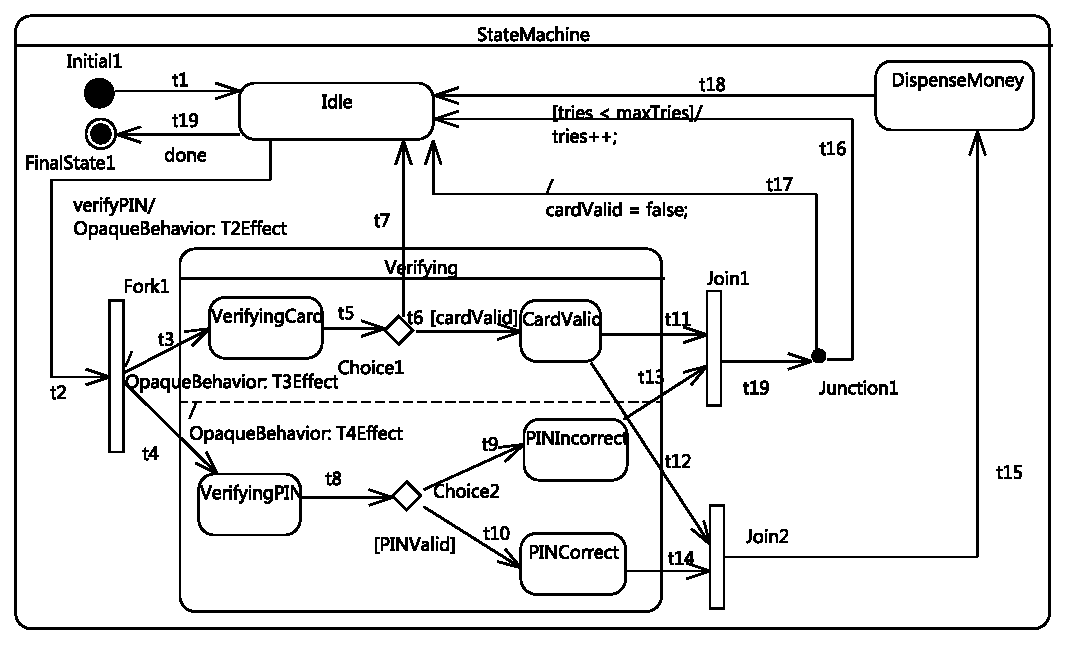
\includegraphics[clip, trim=0.2cm 0.2cm 0.2cm 0.2cm, width=1.0\columnwidth]{figures/ATM.pdf}
	\caption{ATM State machine example} 
	\label{fig:example}
\end{figure}

\section{Background definition}
\label{subsec:background}

%\begin{definition}A directed graph $G = \{V, Ed\}$ consists of a finite set $V$ of vertexes, and a set $Ed$ of edges. An edge connects a source vertex to a target vertex. The source and target vertexes of an edge ed are obtained by $src(ed)$ and $tgt(ed)$.
%\end{definition}

\begin{definition}A UML vertex $v \in V$ has a kind $v.kind \in$  \ti{\{initial, final, state, comp, conc, join, fork, choice, junction, enpoint, expoint, history\}}. 
\end{definition} 

\begin{definition}A region $r \in \mathcal{R}$ is composed of one or several vertexes, and contained by a state $s$. We write $owner(r) = s$ and $vertices(r)$ is its sub-vertices set. 
\end{definition}	

\begin{definition} A vertex is either a UML state or a pseudo-state. A UML state $s$ is a vertex and $s.kind$ $\in$ \{state, comp, conc\}. $s$ has an $entry$, an $exit$ and a $doActivity$ action. A composite state $cs$ contains one or more vertexes. We write $vertices(cs)$ is a set of vertexes contained by $cs$ and, inversely, $owner(v)$ refers to the containing state of the vertex $v$. %A concurrent state contains more than one region.
\end{definition}		

\begin{definition} An action $act$ $\in$ $ActLang$ is a set of statements written in an object-oriented programming language $ActLang$. A guard is a boolean expression written in $ActLang$.
\end{definition}

\begin{definition} A transition $t \in T$ is an edge connecting two vertexes. 
	The source and target vertexes of an edge ed are obtained by $src(t)$ and $tgt(t)$. 
	A transition has a guard $guard(t)$, an effect $effect(t)$, and is associated with a set of events $\subset$ E. We write $events(t)$ as the associated set of events. A transition has a type $t.type$ $\in \{trig, tless, gdless, triggdless\}$ and a kind $t.kind \in {external, local, internal}$.
\end{definition}

\begin{definition} An event is one of the followings:
	\begin{itemize}
		\item A \ti{TimeEvent} $te$ specifies the time of occurrence $d$ relative to a starting time. The latter is specified when a state, which accepts the time event, is entered.
		
		\item A \ti{SignalEvent} $se$ is associated with a signal $sig$, whose data are described by its attributes and is occurred if $sig$ is received by a component, which is an active UML class.
		
		\item A \ti{ChangeEvent} $che$ is associated with a boolean expression $ex(che)$ written in $ActLang$. $che$ is emitted if $ex(che)$ changes from true (false) to false (true).
		
		\item A \ti{CallEvent} $ce$ is associated with an operation $op(ce)$. $ce$ is emitted if there is a call to $op(ce)$.
	\end{itemize}
\end{definition}

\begin{comment}
\begin{definition} A \ti{TimeEvent} $te$ an internal event and specifies the time of occurrence $d$ relative to a starting time. The latter is specified when a state, which accepts the time event, is entered. 
\end{definition}

\begin{definition} A \ti{Signal} $sig$ is data described by its attributes. 
\end{definition}

\begin{definition} A \ti{SignalEvent} $se$ is associated with a signal $sig$ and is occurred if $sig$ is received by a component, which is an active UML class. 
\end{definition}	

\begin{definition}
	A \ti{ChangeEvent} $che$ is associated with a boolean expression $ex(che)$ written in $ActLang$. $che$ is emitted if $ex(che)$ changes from true (false) to false (true).
\end{definition}

\begin{definition}
	A \ti{CallEvent} $ce$ is associated with an operation $op(ce)$. $ce$ is emitted if there is a call to $op(ce)$.
\end{definition}
\end{comment}

Suppose that for each vertex \ti{v} $\in$ $V$, its incoming and outgoing transition lists are extracted by $T_{ins}(v)$ and $T_{outs}(v)$, respectively. %For a list $l$, the function $head$ is used to get the first element of the list. 
If $v.kind = conc$, suppose $regions(v)$ is the region set contained by $v$. %Given a transition t:
%\begin{itemize}
%	\item $t.type = trig$ if $\#events(t) > 0$.
%	\item $t.type = tless$ if $\#events(t) = 0$.
%	\item $t.type = gdless$ if $(guard(t) = true \vee \nexists guard(t)$.
%	\item $t.type = triggdless$ if $\#events(t) = 0 \wedge (guard(t) = true \vee \nexists guard(t))$.
%\end{itemize}

The behavior of an active class $C$ is described by using a state machine whose definition is as following:	

\begin{definition} A state machine sm is a graph specified by $\{V, T\}$ associated with a set of events $E$. A state machine is a special composite state which has no incoming and no outgoing transitions. A root vertex $v$ is a direct sub-vertex of the state machine, $owner(v) = sm$. The set of regions contained by $sm$ is written $\mathcal{R}$.
\end{definition}	

%For each vertex $v$ $\in$ $V$, we write the following sets $T_{ins} (v) = incomings(v), T_{outs}(v) = outgoings(v)$, $t_{first} = head(t_{outs})$; transitive transition sets $T_{ins}^{+}(v)$ and $T_{outs}^{+}(v)$ are sets of transitions incoming to and outgoing from, respectively, $v$ or direct or indirect sub-vertexes of $v$.

\begin{comment}
\begin{strip}
	\begin{equation}
	T_{ins}^{+} (v) =    \left\{
	\begin{array}{ll}
	T_{ins}(v) & v.kind \notin \{comp, conc\}  \\
	T_{ins}(v) \cup \bigcup\limits_{sub \in subvertexes(v)} T_{ins}^{+} (sub) & v.kind \in \{comp, conc\} \\
	\end{array} 
	\right.
	\end{equation}
	
	\begin{equation}
	T_{outs}^{+} (v) =    \left\{
	\begin{array}{ll}
	T_{outs}(v) & v.kind \notin \{comp, conc\}  \\
	T_{outs}(v) \cup \bigcup\limits_{sub \in subvertexes(v)} T_{outs}^{+} (sub) & v.kind \in \{comp, conc\} \\
	\end{array} 
	\right. 
	\end{equation}
\end{strip}
\end{comment}

\begin{definition} Transitive container $owner^+(v)$ of a vertex $v$ of a state machine $sm$ is defined as following:
	\begin{equation}
	owner^+(v) =    \left\{
	\begin{array}{ll}
	sm & owner(v) = sm \\
	owner(v) \cup owner^+(owner(v)) & otherwise\\
	\end{array} 
	\right.
	\end{equation}	
\end{definition}

Likewise, $vertices^+(v)$ is a set of transitive sub-vertexes.

\begin{comment}
In the example in Fig. \ref{fig:example}, we have:
\begin{IEEEeqnarray*}{lCr}	
	owner^+(Idle) = \{StateMachine\}, \\
	owner^+(Choice1) = \{Verifying, StateMachine\}.
\end{IEEEeqnarray*}
\end{comment}

%A state machine $sm = \{V, T\}$ is validated if an associated set of constraints is validated. 
%The set is not presented here due to space limitation.
%is validated if, for each $v \in V$, the constraints listed in Table \ref{table:constraint} are hold. %These are evaluated before the generation phase is taken into account. 

\begin{comment}
\begin{table*}
	\caption{State machine constraints}
	\label{table:constraint}
	\centering
	\begin{tabular}{|p{2.1\columnwidth}|}
	\hline	
	\tabitem If $v.kind = initial$ then $\#T_{outs}(v) = 1 \wedge \#T_{ins}(v) = 0 \wedge t_{first}.type = triggdless$. \\ 
	
	\tabitem If $v.kind = final$ then $\#T_{outs}(v) = 0$. \\
	
	\tabitem If $v.kind \notin \{state, comp, conc\}$ then $\forall t \in T_{outs}(v): src(t) \lnot= tgt(t)$. \\
	
	\tabitem If $T_{auto} = \{t \in T_{outs} | \#events(t) = 0\}$, $T_{ng} = \{t \in T_{auto} | guard(t) = true \vee \nexists guard(t)\}$ then $\#T_{ng} <= 1$. \\
	
	\tabitem $\#T_{ins}^+(v) > 0 \vee \#T_{outs}(v)^+ > 0$. \\
	
	\tabitem If $v.kind = comp$ then $\#subvertexes(v) > 0$. \\
	
	\tabitem If $v.kind = conc$ then $\#regions(v) > 0 \wedge (\forall r \in regions(v): \#subvertexes(r) > 0)$. \\
	
	\tabitem $\#regions(sm) = 1$. \\
	
	\tabitem If $v.kind = fork$ then $\#T_{ins}(v) > 0 \wedge \#T_{outs}(v) > 1 \wedge (\forall t \in T_{outs}(v): t.type = triggdless \wedge owner(tgt(t)).kind = conc)$. \\
	
	\tabitem If $v.kind = join$ then $\#T_{ins} > 1 \wedge \#T_{outs}(v) = 1 \wedge (\forall t \in T_{ins}(v): t.type = triggdless \wedge (\exists s \in owner^+(src(t)), s.kind=conc)) \wedge head(T_{outs}).type = triggdless$. \\
	
	\tabitem If $v.kind \in {choice, junction}$, then $\#T_{ins}(v) > 0 \wedge \#T_{outs}(v) > 1 \wedge (\exists! out \in T_{outs}(v): out.type = gdless)$. \\
	
	\tabitem If $v.kind \in {enpoint, expoint}$, then $owner(v).kind \in \{comp, conc\} \wedge \#T_{ins}(v) > 0 \wedge \#T_{outs}(v) = 1 \wedge head(T_{outs}(v).type = triggdless)$. \\
	
	\tabitem If $v.kind = history$ then $owner(v).kind \in \{comp, conc\} \wedge (if v.kind = comp$ then $\exists! v \in owner(v).subvertexes | v.kind = history) \wedge \#T_{ins} > 0$. \\ \hline
\end{tabular}
\end{table*}	
\end{comment}

\begin{comment}
	\begin{itemize}
		\item If $v.kind = initial$ then $\#T_{outs}(v) = 1 \wedge \#T_{ins}(v) = 0 \wedge t_{first}.type = triggerguardless$. 
		
		\item If $v.kind = final$ then $\#T_{outs}(v) = 0$.
		
		\item If $v.kind \notin \{state, comp, conc\}$ then $\forall t \in T_{outs}(v): src(t) \lnot= tgt(t)$. 
		
		\item If $T_{auto} = \{t \in T_{outs} | \#events(t) = 0\}$, $T_{ng} = \{t \in T_{auto} | guard(t) = true \vee \nexists guard(t)\}$ then $\#T_{ng} <= 1$.
		
		\item $\#T_{ins}^+(v) > 0 \vee \#T_{outs}(v)^+ > 0$.
		
		\item If $v.kind = comp$ then $\#subvertexes(v) > 0$. 
		
		\item If $v.kind = conc$ then $\#regions(v) > 0 \wedge (\forall r \in regions(v): \#subvertexes(r) > 0)$. 
		
		\item $\#regions(sm) = 1$.
		
		\item If $v.kind = fork$ then $\#T_{ins}(v) > 0 \wedge \#T_{outs}(v) > 1 \wedge (\forall t \in T_{outs}(v): t.type = triggerguardless \wedge owner(tgt(t)).kind = conc)$.
		
		\item If $v.kind = join$ then $\#T_{ins} > 1 \wedge \#T_{outs}(v) = 1 \wedge (\forall t \in T_{ins}(v): t.type = triggerguardless \wedge (\exists s \in owner^+(src(t)), s.kind=conc)) \wedge head(T_{outs}).type = triggerguardless$.
		
		\item If $v.kind \in {choice, junction}$, then $\#T_{ins}(v) > 0 \wedge \#T_{outs}(v) > 1 \wedge (\exists! out \in T_{outs}(v): out.type = guardless)$.
		
		\item If $v.kind \in {enpoint, expoint}$, then $owner(v).kind \in \{comp, conc\} \wedge \#T_{ins}(v) > 0 \wedge \#T_{outs}(v) = 1 \wedge head(T_{outs}(v).type = triggerguardless)$.
		
		\item If $v.kind = history$ then $owner(v).kind \in \{comp, conc\} \wedge (if v.kind = comp then \exists! v \in owner(v).subvertexes | v.kind = history) \wedge \#T_{ins} > 0$.
	\end{itemize}	
\end{comment}
\begin{comment}
\begin{definition} A transition graph $\tau$ is an acyclic directed graph ($\mathcal{T}$, $\mathcal{P}$, $\mathcal{T}$) where $\mathcal{S}, \mathcal{L}, \mathcal{P}$ are sets of vertexes and $\mathcal{T}$ is a set of transitions whose source and target vertexes belong to $\mathcal{S} \cup \mathcal{L} \cup \mathcal{P}$. And following conditions are satisfied:
\begin{itemize}
	\item $\forall s \in \mathcal{S} \cup \mathcal{L}$:
		\begin{itemize}
			\item If $s \in \mathcal{S}$ then $s$ is a state.
			\item Otherwise $s$ is a state or $s.kind = final$.
		\end{itemize}
	\item $\forall p \in \mathcal{P}, p.kind \notin \{state, comp, conc\}$.	
\end{itemize}	
$\mathcal{S}$ and $\mathcal{L}$ are sets of source and reachable target states of $\tau$, respectively.  
\end{definition}

A transition graph is composed of one or multiple compound transitions, each of which consists of one/multiple transitions starting from states/pseudo states/pseudo states to pseudo states/states/pseudo states. A state machine can contain multiple transition graphs. Fig. \ref{fig:transitionGraph} (a) and (b) show two transition graphs $\tau_{1}$ and $\tau_{2}$ of the ATM state machine, respectively, in which 
\begin{IEEEeqnarray*}{lCr}
	\tau_{1} &=& (\mathcal{S}_1, \mathcal{L}_1, \mathcal{P}_1, \mathcal{T}_1) = (\{Idle\}, \{VerifyingCard, \\ 
	&& {} VerifyingPIN\}, \{Fork1\}, \{t2, t3, t4\})
\end{IEEEeqnarray*}
and
\begin{IEEEeqnarray*}{lCr}	
	\tau_{2} &=& (\mathcal{S}_2, \mathcal{L}_2, \mathcal{P}_2, \mathcal{T}_2) = (\{CardValid, PINIncorrect\}, \\ 
	&& {} \{Idle\}, \{Join2, Choice3\}, \{t11, t13, t19, t16, t17\}).
\end{IEEEeqnarray*}



\begin{figure}
	\centering
	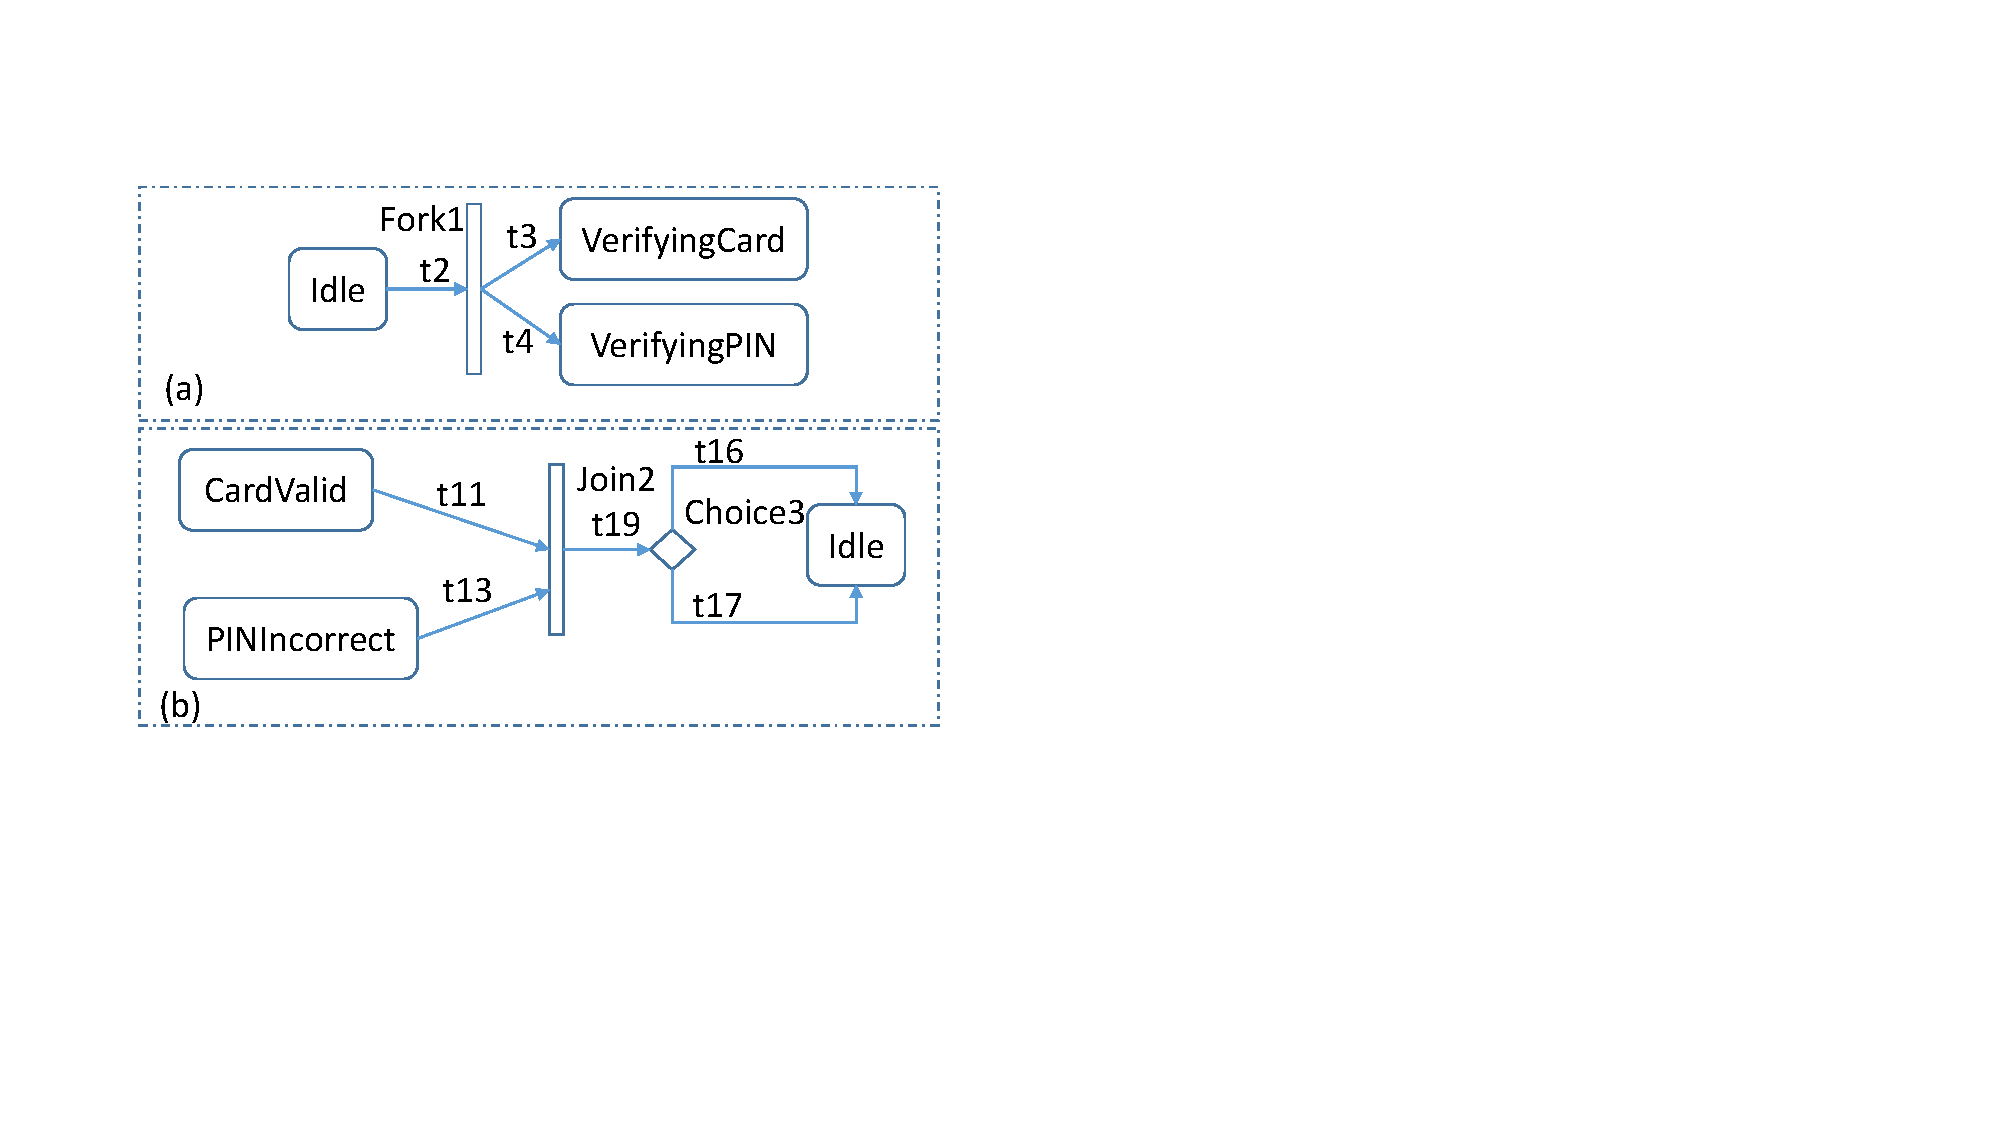
\includegraphics[clip, trim=2.0cm 6cm 17.5cm 3cm, width=\columnwidth]{figures/transitionGraph.pdf}
	\caption{Transition graphs} 
	\label{fig:transitionGraph}
\end{figure}


\begin{definition} A compound transition $t_{cp}$ is a virtual path which starts from one or multiple UML state and ends on one or multiple UML state. A compound transition is specified by a triple \{srcs($t_{cp}$), trc($t_{cp}$), tgts($t_{cp}$)\}, in which source part srcs($t_{cp}$) consists of one or multiple states, transition part trc($t_{cp}$) consists of multiple transitions, and target part tgts($t_{cp}$) consists of one or multiple states. 
\end{definition}


Given a state, Algorithm \ref{alg:cptransition} presents how to calculate transition graphs whose source $t_{cp}$ whose source part contains only a state $s$. 

\begin{algorithm}[]
	\caption{Transition graphs calculation
		\label{alg:cptransition}}
	\begin{algorithmic}[1]
		\Require{A state $s$ of a state machine}
		\Ensure{A set of transition graphs $\mathcal{GT}$}
		\Procedure{calculateTransGraphs}{$s$}
		\Let{$\mathcal{GT}$}{$\emptyset$} 
		\For {$out \in T_{outs}(s)$}
			\If {$tgt(out)$ is not a state}
				\Let{$\tau$}{($\mathcal{S}$, $\mathcal{L}$, $\mathcal{P}$, $\mathcal{T}$) $=\{\emptyset,\emptyset, \emptyset, \emptyset\}$}
				\Let{$\mathcal{P}$}{$\mathcal{P} \cup {tgt(out)}$}
				\Let{$\mathcal{S}$}{$\mathcal{S} \cup \{s\}$}
				\Let{$\mathcal{T}$}{$\mathcal{T} \cup {out}$}
				\If {$tgt(out).kind = join$}
					\Let{$ins$}{\\$\{i \in T_{ins}(tgt(out))| owner(src(i)) = owner(s)\}$}
					\Let{$\mathcal{S}$}{$\mathcal{S} \cup \{src(i)|i \in ins\}$}
					\Let{$\mathcal{T}$}{$\mathcal{T} \cup ins$}
				\EndIf
				\Let{$nexts$}{$FINDTRANS(tgt(out))$}
				\Let{$\mathcal{T}$}{$\mathcal{T} \cup nexts$}
				\Let{H}{\\$\{tgt(t)|t \in nexts \wedge tgt(t).kind = history\}$}
				\Let{$\mathcal{P}$}{$\mathcal{P} \cup \{src(t)|t \in nexts\} \cup H$}
				\Let{$\mathcal{L}$}{$\mathcal{L} \cup \{tgt(t)|t \in nexts \wedge tgt(t)$ is state $\}$}
								
				\Let{$\mathcal{GT}$}{$\mathcal{GT} \cup \{\tau\}$} 
			\EndIf
		\EndFor
		\EndProcedure
		
		\Require{A vertex $v$}
		\Ensure{Transition paths starting from $v$ and ending on a state}
		\Procedure{FindTrans}{$v$}
		\Let{$nextTrans$}{$T_{outs}(v)$}
		\For {$out \in T_{outs}(v)$}
			\If {$tgt(out)$ is not a state}
				\Let {$nextTrans$}{\\$nextTrans \cup FINDTRANS(tgt(out))$}
			\EndIf
		\EndFor	 			 	
		\Return {$nextTrans$} 
		\EndProcedure	
	\end{algorithmic}
\end{algorithm}

For example, applying this algorithm to all states of the state machine example in \ref{fig:example}, we can calculate other transition graphs which are:
\begin{IEEEeqnarray*}{lCr}
	\tau_{3} &=& (\mathcal{S}_3, \mathcal{L}_3, \mathcal{P}_3, \mathcal{T}_3) = (\{VerifyingCard\}, \{Idle, \\ 
	&& {} CardValid\}, \{Choice1\}, \{t5, t6, t7\}),
\end{IEEEeqnarray*}
\begin{IEEEeqnarray*}{lCr}	
	\tau_{4} &=& (\{VerifyingPIN\}, \{PINIncorrect, \\
	&& {} PINCorrect\}, \{Choice2\}, \{t8, t9, t10\}),
\end{IEEEeqnarray*} 
and
\begin{IEEEeqnarray*}{lCr}	
	\tau_{5} &=& (\{CardValid, PINCorrect\}, \{DispenseMoney\}, \\ 
	&& {} \{Join2\}, \{t12, t14, t15\}).
\end{IEEEeqnarray*} 

\end{comment}

\begin{comment}
\begin{definition} A transition graph $\tau$ is an acyclic directed graph ($\mathcal{T}_r$, $\mathcal{P}$, $\mathcal{T}$) where $\mathcal{P}$ is a set of vertexes, and $\mathcal{T}_{r}$ and $\mathcal{T}$ are sets of transitions. $\mathcal{T}_{r}$ is called the set of root transitions of the graph. Following conditions are satisfied:
	\begin{itemize}
		\item $\forall t \in \mathcal{T}_r, src(t)$ is a state.
		
		\item $\forall p \in \mathcal{P}, p.kind \notin \{state, comp, conc\}$.	
		
		\item $\forall t \in \mathcal{T}, src(t)$ is a pseudo state.
	\end{itemize}	
\end{definition}

A traversal from the root transitions of a transition graph to a stable state configuration is a compound transition. A state machine can contain multiple transition graphs. Fig. \ref{fig:transitionGraph} (a) and (b) show two transition graphs $\tau_{1}$ and $\tau_{2}$ of the ATM state machine, respectively, in which 
\begin{IEEEeqnarray*}{lCr}
	\tau_{1} &=& (\mathcal{T}_r, \mathcal{P}, \mathcal{T}) = (\{t2\}, \{Fork1\}, \{t3, t4\} )
\end{IEEEeqnarray*}
and
\begin{IEEEeqnarray*}{lCr}	
	\tau_{2} &=& (\{t11, t13\}, \{Join2, Choice3\}, \{t19, t16, t17\}).
\end{IEEEeqnarray*}



\begin{figure}
	\centering
	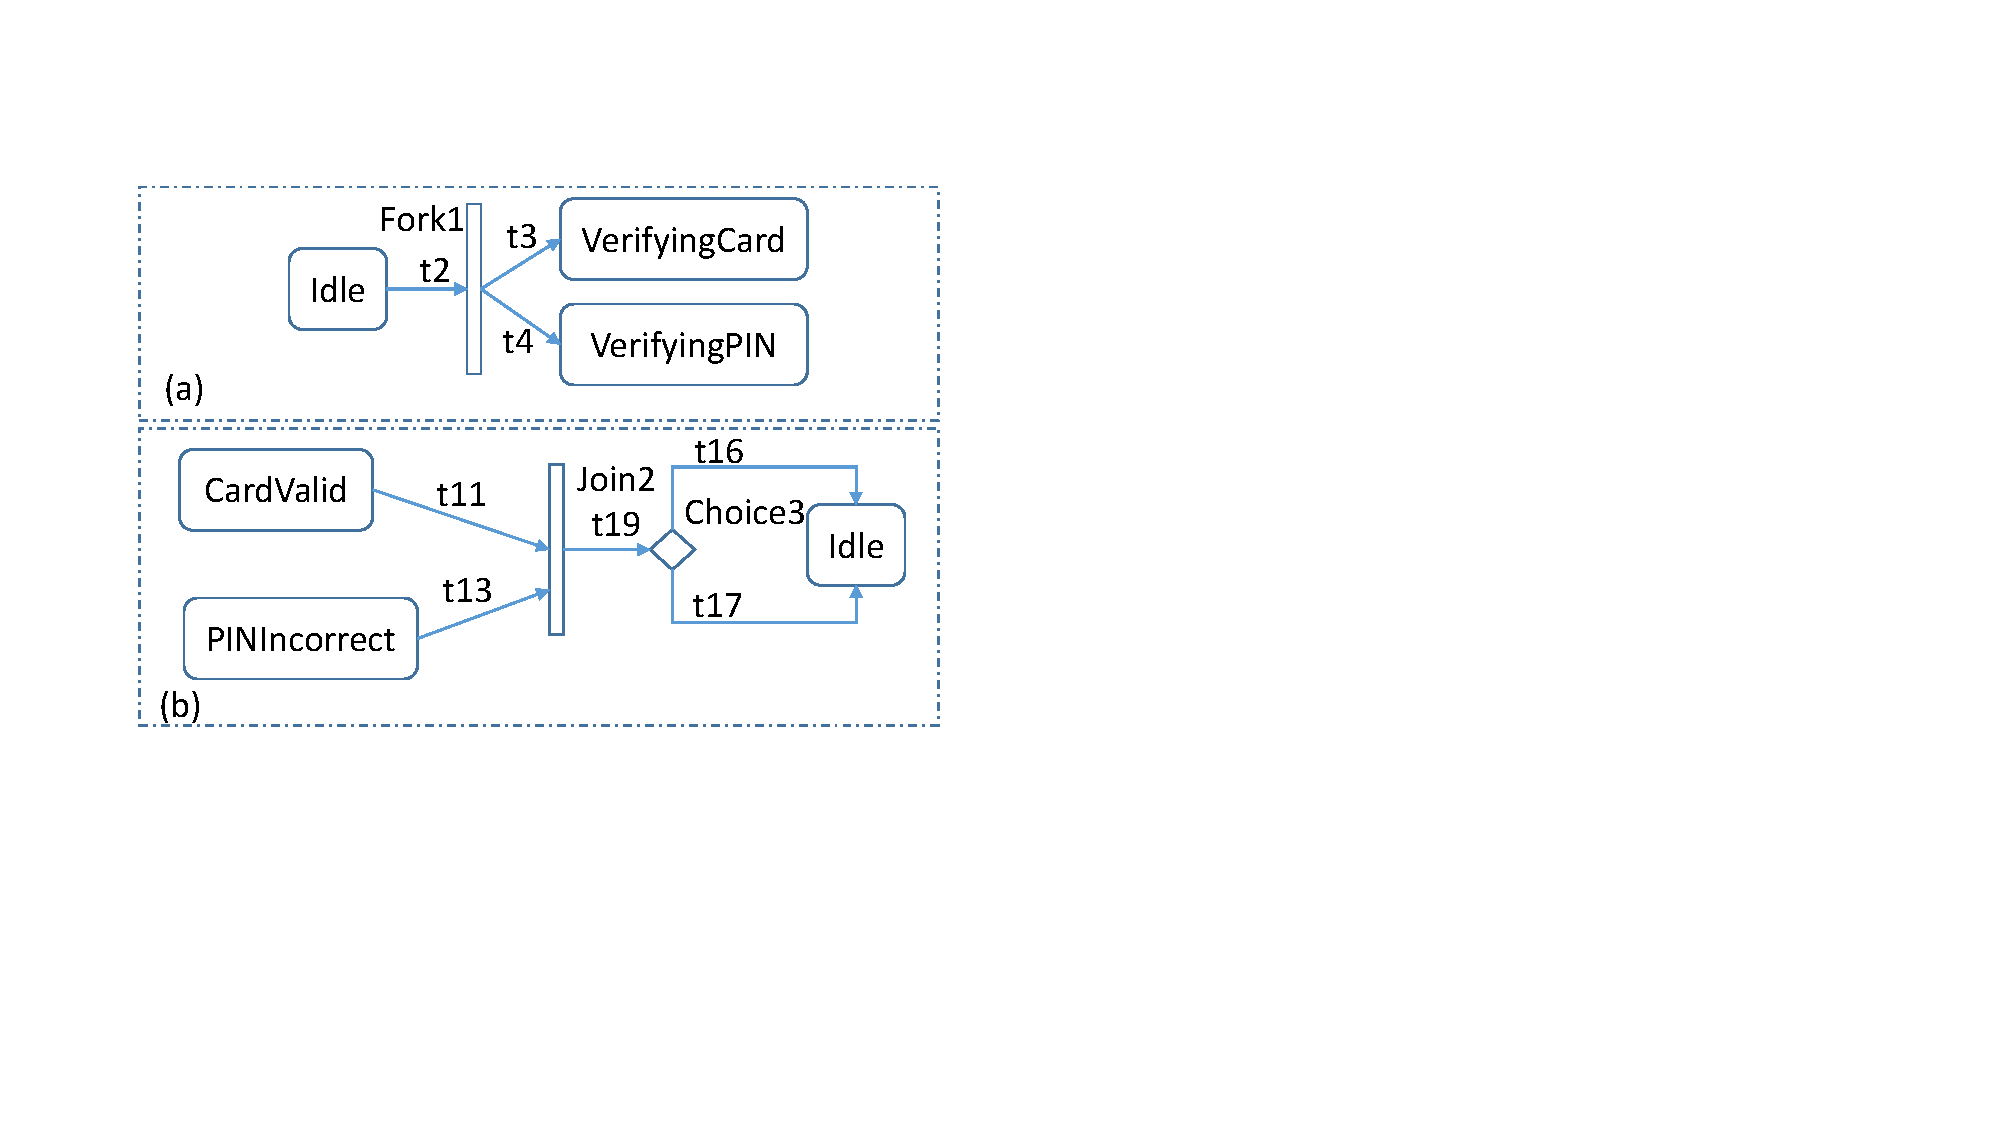
\includegraphics[clip, trim=2.0cm 6cm 17.5cm 3cm, width=\columnwidth]{figures/transitionGraph.pdf}
	\caption{Transition graphs} 
	\label{fig:transitionGraph}
\end{figure}



Given a state, Algorithm \ref{alg:cptransition} presents how to calculate transition graph set whose root transitions outgo from $s$. 

\begin{algorithm}[]
	\caption{Transition graphs calculation
		\label{alg:cptransition}}
	\begin{algorithmic}[1]
		\Require{A state $s$ of a state machine}
		\Ensure{A set of transition graphs $\mathcal{GT}$}
		\Procedure{calculateTransGraphs}{$s$}
		\Let{$\mathcal{GT}$}{$\emptyset$} 
		\For {$out \in T_{outs}(s)$}
			\If {$tgt(out)$ is not a state}
				\Let{$\tau$}{($\mathcal{T}_r$, $\mathcal{P}$, $\mathcal{T}$) $=\{\emptyset,\emptyset, \emptyset\}$}
				\Let{$\mathcal{P}$}{$\mathcal{P} \cup {tgt(out)}$}
				\Let{$\mathcal{T}_r$}{$\mathcal{T}_r \cup {out}$}
			\If {$tgt(out).kind = join$} 
				\Let{$\mathcal{T}_r$}{$\mathcal{T}_r \cup T_{ins}(tgt(out))$}
			\EndIf
				\Let{$nexts$}{$FINDTRS(tgt(out))$}
				\Let{$\mathcal{T}$}{$\mathcal{T} \cup nexts$}
			
				\Let{$\mathcal{GT}$}{$\mathcal{GT} \cup \{\tau\}$} 
			\EndIf
		\EndFor
		\EndProcedure
		
		\Require{A vertex $v$}
		\Ensure{Transition paths starting from $v$ to atomic  states}
		\Procedure{FINDTRS}{$v$}
		\Let{$outs$}{$T_{outs}(v)$}
		\For {$out \in T_{outs}(v)$}
			\If {$tgt(out)$ is not a state}
				\Let {$outs$}{\\$outs \cup FINDTRS(tgt(out))$}
			\ElsIf $tgt(out).kind \in {comp, conc}$
				\For {$sub \in subvertexes(tgt(out)), sub.kind=initial$}
					\Let {$outs$}{$outs \cup FINDTRS(sub)$}
				\EndFor
			\EndIf 
		\EndFor	 			 	
		\Return {$outs$} 
		\EndProcedure	
	\end{algorithmic}
\end{algorithm}

For example, applying this algorithm to all states of the state machine example in \ref{fig:example}, we can calculate other transition graphs which are:
\begin{IEEEeqnarray*}{lCr}
	\tau_{3} &=& (\mathcal{S}_3, \mathcal{L}_3, \mathcal{P}_3, \mathcal{T}_3) = (\{VerifyingCard\}, \{Idle, \\ 
	&& {} CardValid\}, \{Choice1\}, \{t5, t6, t7\}),
\end{IEEEeqnarray*}
\begin{IEEEeqnarray*}{lCr}	
	\tau_{4} &=& (\{VerifyingPIN\}, \{PINIncorrect, \\
	&& {} PINCorrect\}, \{Choice2\}, \{t8, t9, t10\}),
\end{IEEEeqnarray*} 
and
\begin{IEEEeqnarray*}{lCr}	
	\tau_{5} &=& (\{CardValid, PINCorrect\}, \{DispenseMoney\}, \\ 
	&& {} \{Join2\}, \{t12, t14, t15\}).
\end{IEEEeqnarray*} 

\end{comment}
\begin{definition} Current active configuration $Cfg$ of a UML state machine sm is a set of candidate UML states which are able to process an incoming event. 
\end{definition}







\begin{comment}
\section{Thread-based Concurrency}
\label{sec:thread}
\subsection{Thread-based concurrency analysis} 

While concurrency is an important aspect defined by the UML State machine specification, especially hierarchical and concurrent state machines with \ti{doActivity}s for states, most of existing approaches do not take into account. This is non-trivial since concurrency is dynamic in UML state machine since the number of threads used for concurrency is non-deterministic.

Let us give an analysis on the state machine example in Fig. \ref{fig:example}. Assuming that \ti{Idle} is the current active state and a \ti{verifyPIN} event is coming. 
The \ti{doActivity} behavior of \ti{Idle} \ti{doActivity(Idle)} (if has) is terminated, \ti{exit(Idle)} and the \ti{effect(t2)} (\ti{T2Effect}) are executed sequentially. 
These actions are run in a state machine main thread which reads incoming events from a "first in, first out" (FIFO) priority queue. 
Fig. \ref{fig:threading1} shows the activity diagram representing the concurrency processing \ti{verifyPIN}, in which each partition represents a thread. 
\ti{effect(t3)} and \ti{effect(t3)} are run concurrently in two threads \ti{T3Run} and \ti{T4Run}, respectively, since the transitions owning these effects outgo from a fork pseudo state. 
The entry action \ti{entry(Verifying)} is executed following the termination of the two threads. 

UML says that \ti{doActivity(Verifying)}, \ti{entry(VerifyingCard)} and \ti{entry(VerifyingPIN)} should be concurrently executed upon the completion of \ti{entry(Verifying)}, which is represented by a fork node, in which a \ti{Start} signal is sent to \ti{VerifyingDoRun} in order for commencing \ti{doActivity(Verifying)}. 
The executions of the \ti{doActivity}s of the states \ti{VerifyingCard} and \ti{VerifyingPIN} are also concurrent. 
Also, upon the completion of \ti{entry(VerifyingCard)} and \ti{entry(VerifyingPIN)}, the main thread completes the processing of the \ti{verifyPIN} event, reads next events from the queue or waits for next event occurrences.

\begin{figure}
	\centering
	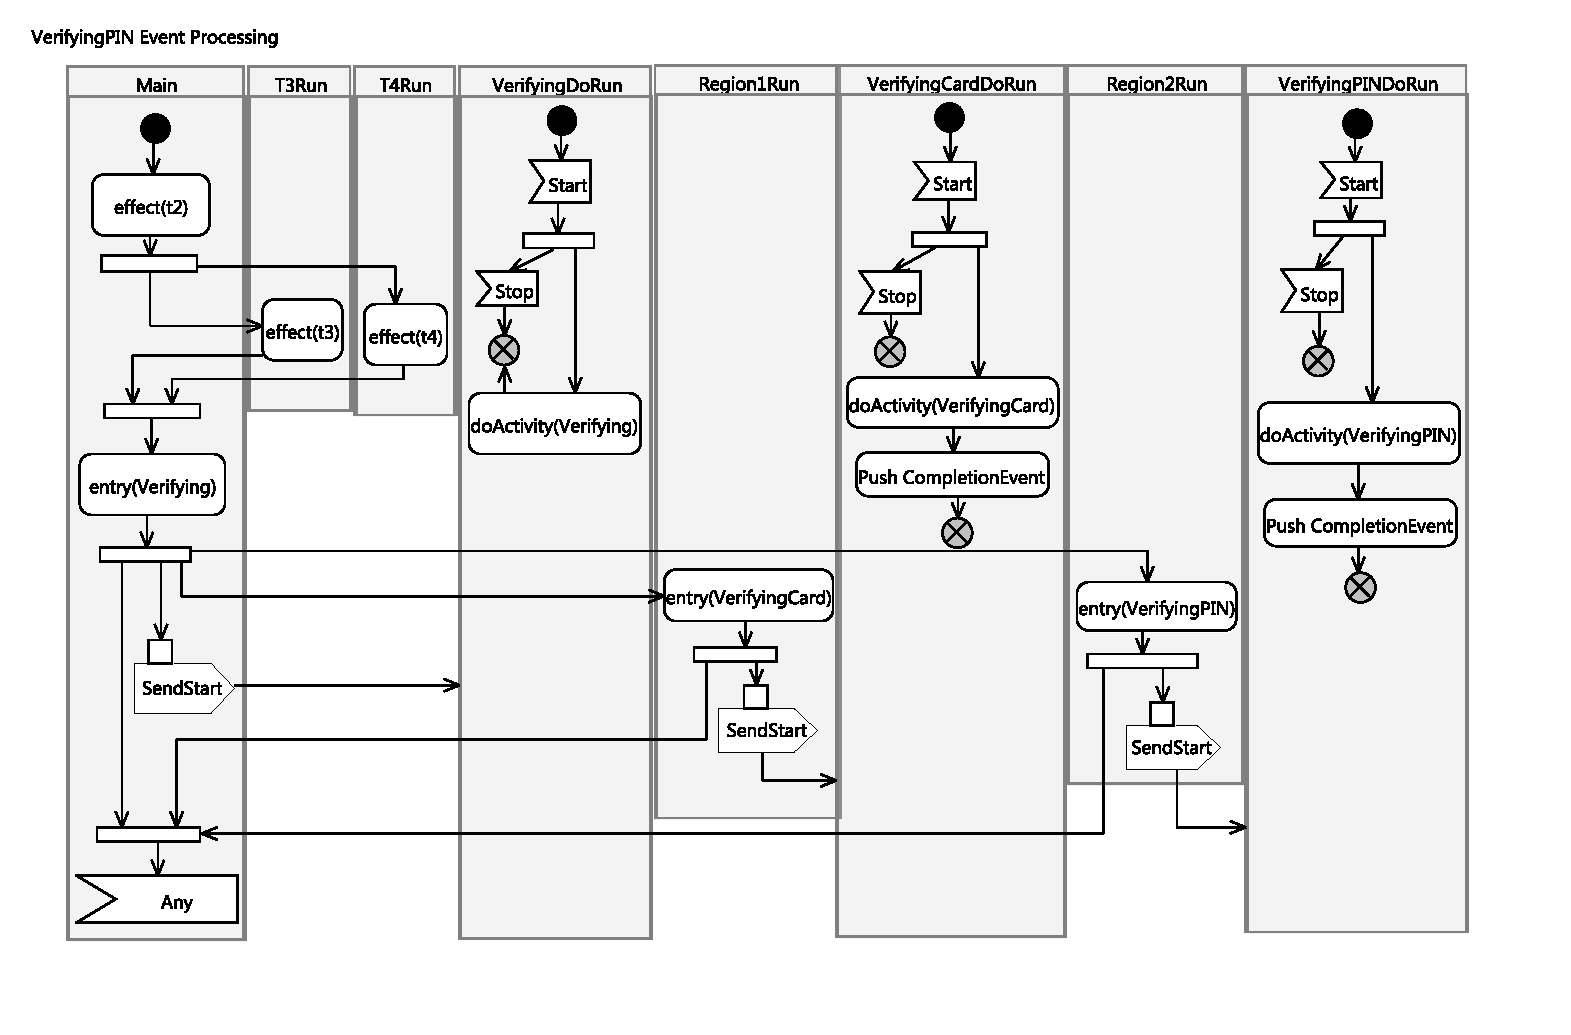
\includegraphics[clip, trim=1.0cm 1.6cm 1.6cm 1cm, width=1.03\columnwidth]{figures/ThreadingExample.pdf}
	\caption{Concurrency of the ATM when receiving the \ti{verifyingPIN} event} 
	\label{fig:threading1}
\end{figure}

If no event is coming, and \ti{doActivity(VerifyingCard)} and \ti{doActivity(VerifyingPIN)} are long actions (e.g. forever loops inside), the state machine remains its active configuration and three concurrent actions including \ti{CheckForEvents}, \ti{doActivity(VerifyingCard)}, and \ti{doActivity(VerifyingPIN)} are permanently run.

The termination time of \ti{doActivity(VerifyingCard)} and \ti{doActivity(VerifyingPIN)} is non-deterministic. 
However, a completion event is generated and pushed to the event queue whenever one of the two completes. 
For illustration, assuming that \ti{doActivity(VerifyingCard)} terminates before \ti{doActivity(VerifyingPIN)}. 
As in Fig. \ref{fig:threading2}, the Main thread checks the \ti{CompletionEvent}. \ti{exit(VerifyingCard)} and \ti{effect(t5)} are then executed sequentially. If \ti{cardValid} is computed as true as the result of \ti{doActivity(VerifyingCard)} and \ti{exit(VerifyingCard)}, the Main thread simply executes \ti{effect(t6)} and \ti{entry(CardValid)} before waiting for other events.

In contrast, Main sends a signal to stop \ti{doActivity(VerifyingPIN)} and \ti{doActivity(Verifying)}, executes exit, transition and entry actions in an appropriate order (see Fig. \ref{fig:threading2}) and waits for other events.

We see that the number of concurrent actions is not constant but changes timely. 
Each action can either deterministically or non-deterministically terminate. 
In this sense, deterministic actions (DAs) prevent the Main thread from going to the waiting-for-event point. 
In other words, pending events in the queue are only read and processed once all deterministic actions complete. Therefore, we re-define the run-to-completion paradigm of UML state machine as following:
 
\begin{definition}
	Run-to-completion means that, in the absence of exceptions or asynchronous destruction of the context	class object or the state machine execution, a pending Event occurrence is dispatched only after the completion of all deterministic actions commenced by the processing of the current event. 
	At this point, a stable state configuration has been reached
\end{definition}

In the example, some of DAs are as followings: \ti{effect(t2)}, \ti{effect(t4)}, \ti{entry(Verifying)}, \ti{entry(VerifyingCard)}, and non-deterministic actions (NDAs) as followings: \ti{doActivity(Verifying)}, \ti{doActivity(VerifyingCard)} and \ti{doActivity(VerifyingPIN)}.


\begin{figure}
	\centering
	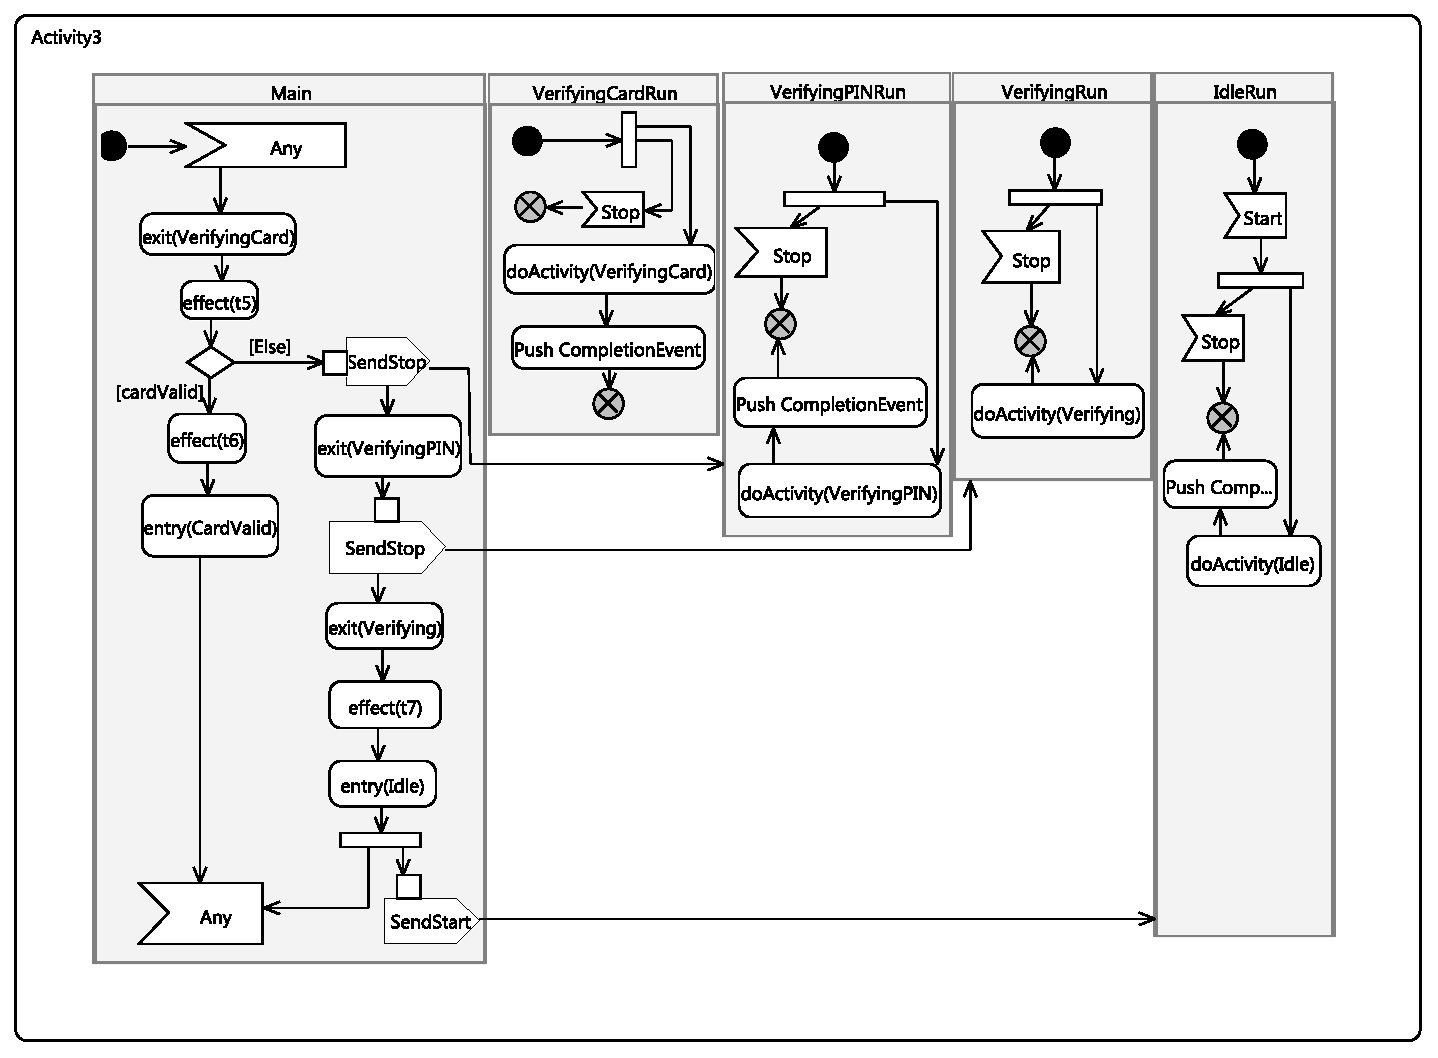
\includegraphics[clip, trim=1.5cm 1.6cm 1.6cm 1.2cm, width=1.03\columnwidth]{figures/ThreadingExample2.pdf}
	\caption{Concurrency of the ATM when \ti{doActivity} of \ti{VerifyingCard} completes before that of \ti{VerifyingPIN}}
	\label{fig:threading2}
\end{figure}

\subsection{Thread-based design of generated code}
Each NDA is run in parallel with the main thread which reads and dispatch events from the event queue. 
Each is associated with a thread which is initialized at the state machine initialization moment. 
The number of threads associated with NDAs is therefore equal to that of the NDAs.
The design of threads is based on the thread pool pattern, which initializes all threads at once, and the paradigm "wait-execute-wait". 
In the latter, a thread \tb{waits} for a signal to \tb{execute} its associated method and goes back to the \tb{wait} point if it receives a stop signal or its associated method completes. 
An NDA is one of the followings:
\begin{itemize}
	\item \ti{doActivity} of each state if has. The number of \ti{doActivity} $n_{do} = \#\{s \in V|\exists doActivity(s)\}$
	
	\item Sleep function associated with a \ti{TimeEvent} which counts ticks and emits a \ti{TimeEvent} once completes: $n_{te} = \#\{e \in E|\ti{e is a time event}\}$.
	
	\item Change detect function associated with a \ti{ChangeEvent} which observes a variable or a boolean expression and pushes an event to the queue if changes happen: $n_{che} = \#\{e \in E|\ti{e is a change event}\}$.
\end{itemize} 

Therefore, the concurrency has the number of initial threads $n_{threads} = n_{do} + n_{te} + n_{che}$ plus a main thread which reads events from the event queue, and sends start and stop signals to these initial threads. 

Now we consider spontaneous threads which are created to run DAs, joined until and destroyed once DAs complete. 
\end{comment}
\begin{comment}
The followings describe different types of DAs:

\begin{itemize}
	\item Actions executed when entering/exiting an orthogonal region, which can be: execute a chain of transition effects contained by the region before entering a stable sub-state or exiting the region completely.%: $n_{region threads} = \#\{r \in \mathcal{R}|ctner(r).kind=conc\}$
	
	\item Effects of transitions outgoing from a $fork$ and those incomings to a $join$.%: \\
	%$\mathcal{J} = \{v \in V|v.kind=join\}$ \\
	%$\mathcal{F} = \{v \in V|v.kind=fork\}$ \\
	%$$n_{FJ\_threads} = \sum_{v \in \mathcal{F}} {\#T_{outs}(v)} + \sum_{v \in \mathcal{J}} {\#T_{ins}(v)}$$.
\end{itemize}
%\end{comment}
\begin{comment}
The spontaneous threads follow a paradigm in which if a thread $parent$ creates a set of threads $children$, $parent$ must wait until $children$ complete their associate methods. These threads are created in one of the following cases:

\begin{itemize}
	\item A thread is created for each effect of transitions' outgoing from a \ti{fork} or incoming to a \ti{join}.
	
	\item Entering a concurrent state $s$, after the execution of $entry(s)$, a thread is also created for each orthogonal region. 
	
	\item Exiting a concurrent state $s$, before the execution of $exit(s)$, a thread is also created for each region to exit the corresponding active sub-state.
	
	\item An event is processed by active states, in which a thread per orthogonal region. 
\end{itemize}

\subsection{Deadlock avoidance}
Each NDA thread is associated with a mutex for synchronization communication in the multi-thread-based generated code. 
The mutex must be locked before the method associated with the thread is executed. 
The mutex associated with the main thread protects the run-to-completion semantics since some event such as \ti{CallEvent} can be processed synchronously and some asynchronously. Each event processing must lock the main mutex before executing the actual processing. 
%Deadlock is one of the main issues in designing multi-thread applications, in which two competing actions wait for the other to finish. In our case, 
\end{comment}

\begin{comment}
\begin{tabular}{p{4.0cm}|p{4.0cm}}
Example code generated for doActivity  &  Option  2\\
\begin{lstlisting}[language=C++]
void doActivity(int stateId) {
  isStarts[stateId] = false;
  while(true) {
    mutex[stateId].lock();
    while(!isStarts[stateId]) {
      mutex[stateId].wait();
    }
    states[stateId].doActivity();
    isStarts[stateId] = false;
    mutex[stateId].unlock();
    if (!isStops[stateId]) {
      if (stateId == IDLE_ID || stateId == DISPENSEMONEY_ID ...) {
	    pushCompletionEvent(stateId);
	  }
    }
  }
}
	\end{lstlisting}&
	\begin{lstlisting}
	#include <stdio.h>
	
	int main()
	{
	printf("Hello world\n");
	}
	\end{lstlisting}
\end{tabular} 
\end{comment}
















\section{Thread-based Concurrency}
\label{sec:thread}
This section describes our design of concurrency for generated code. 
%The design is based on an example-based analysis, which is not presented here due to space limitation.

%\input{sections/analysis}
\subsection{Thread-based design of generated code}
The concurrency of concurrent USMs is based on multi-thread, in which there are permanent and spontaneous threads. 
While permanent threads (PTs) are created once and live as long as the state machine is alive, spontaneous threads (STs) are spawned and active for a while. 
%The method associated with a permanent thread is a non-deterministic action, which is run in parallel with the main thread. The latter reads and dispatch events from the event queue. 
Each PT is initialized at the state machine initialization. 
%The number of threads associated with NDAs is therefore equal to that of the NDAs.
The design of threads is based on the thread pool pattern, which initializes all threads at once, and the paradigm "wait-execute-wait". 
In the latter, a thread \tb{waits} for a signal to \tb{execute} its associated method and goes back to the \tb{wait} point if it receives a stop signal or its associated method completes. 
Each PT is associated with one of the following actions:
\begin{itemize}
	\item \ti{doActivity} of each state if has any. %The number of \ti{doActivity} $n_{do} = \#\{s \in V|\exists doActivity(s)\}$
	
	\item Sleep function associated with a \ti{TimeEvent} which counts ticks and emits a \ti{TimeEvent} once completes.%: $n_{te} = \#\{e \in E|\ti{e is a time event}\}$.
	
	\item Change detect function associated with a \ti{ChangeEvent} which observes a variable or a boolean expression and pushes an event to the queue if a change occurs.%: $n_{che} = \#\{e \in E|\ti{e is a change event}\}$.
	
	\item State machine main thread,which reads events from the event queue, and sends start and stop signals to other PTs.
\end{itemize} 

%Therefore, The number of initial threads is $n_{threads} = n_{do} + n_{te} + n_{che}$ plus a main thread, which reads events from the event queue, and sends start and stop signals to these initial threads. 

Now we consider STs which are spawned by a parent thread, joined until and destroyed once the associated methods complete. 

\begin{comment}
The followings describe different types of DAs:

\begin{itemize}
\item Actions executed when entering/exiting an orthogonal region, which can be: execute a chain of transition effects contained by the region before entering a stable sub-state or exiting the region completely.%: $n_{region threads} = \#\{r \in \mathcal{R}|ctner(r).kind=conc\}$

\item Effects of transitions outgoing from a $fork$ and those incomings to a $join$.%: \\
%$\mathcal{J} = \{v \in V|v.kind=join\}$ \\
%$\mathcal{F} = \{v \in V|v.kind=fork\}$ \\
%$$n_{FJ\_threads} = \sum_{v \in \mathcal{F}} {\#T_{outs}(v)} + \sum_{v \in \mathcal{J}} {\#T_{ins}(v)}$$.
\end{itemize}
\end{comment}

The STs follow a paradigm in which if a thread $parent$ spawns a set of threads $children$, $parent$ must wait until $children$ complete their associated methods. These threads are spawned in one of the following cases:

\begin{itemize}
	\item A thread is created for each effect of transitions outgoing from a \ti{fork} or incoming to a \ti{join}.
	
	\item Entering a concurrent state $s$, after the execution of $entry(s)$, a thread is created for each orthogonal region. 
	
	\item Exiting a concurrent state $s$, before the execution of $exit(s)$, a thread is also created for each region to exit the corresponding active sub-state.
	
	%\item An event is processed by active states, in which a thread per orthogonal region. 
\end{itemize}

\subsection{Deadlock avoidance}
Each PT is associated with a mutex for synchronization communication in the multi-thread-based generated code. 
The mutex must be locked before the method associated with the thread is executed. 
The mutex associated with the main thread preserves the run-to-completion semantics since some event such as \ti{CallEvent} can be processed synchronously and some asynchronously. Each event processing must lock the main mutex before executing the actual processing. 
%Deadlock is one of the main issues in designing multi-thread applications, in which two competing actions wait for the other to finish. In our case, 


\begin{comment}
\begin{tabular}{p{4.0cm}|p{4.0cm}}
Example code generated for doActivity  &  Option  2\\
\begin{lstlisting}[language=C++]
void doActivity(int stateId) {
isStarts[stateId] = false;
while(true) {
mutex[stateId].lock();
while(!isStarts[stateId]) {
mutex[stateId].wait();
}
states[stateId].doActivity();
isStarts[stateId] = false;
mutex[stateId].unlock();
if (!isStops[stateId]) {
if (stateId == IDLE_ID || stateId == DISPENSEMONEY_ID ...) {
pushCompletionEvent(stateId);
}
}
}
}
\end{lstlisting}&
\begin{lstlisting}
#include <stdio.h>

int main()
{
printf("Hello world\n");
}
\end{lstlisting}
\end{tabular} 
\end{comment}



\section{Code generation pattern}
\label{sec:codegen}
%\subsection{Transformation pattern}
%todo: describe the pattern

%Transformation from State machine to fUML (classes, attributes, methods)
%\lipsum[1]

\subsection{Assumption}
%todo: give some assumptions on code generation such as functions to create methods, attriutes, classes
Assuming that we want to generate from the state machine to an object oriented programming language $ActLang$, which is a C++-like and supports multi-threading by following functions and resource control as mutexes.
\begin{itemize}
	%\item $genClass(n, generals, itfs)$ creates a class with its name, parent class set, and implemented interfaces as \ti{n}, \ti{generals}, and \ti{itfs}.
	
	%\item $genMtd(n, c, type, params)$ creates a method $m$ with its name as $n$ inside the class $c$, its return type as $type$, and $params$ as its parameter set.
	
	%\item $genAttr(n, c, type, multiplicity)$ creates an attribute named $n$ in the class $c$ and typed by $type$. The create attribute is an array if $multiplicity > 1$, otherwise a simple attribute.
	
	%\item $genEnum(n)$ and $genEnumLit(enum, n)$ create an enumeration and its enumeration literal, respectively.
	
	%\item $genBody(m, body)$ adds a body to a method. The body is a string which contains a list of statements.
	
	%\item $createParalle(t, seg)$ generates a mechanism which allows the segment code $seg$ run in a thread $t$. Similarly, $genWait(t), genJoin(t)$.
	
	\item A mutex has three methods $lock$, $unlock$, and $wait$, which automatically unlocks the mutex and waits until it receives a signal.  
	
	%\item $synchronize(seg)$ generates a mechanism which allows the segment code $seg$ run safely (can be either based on \ti{POSIX pthread} or \ti{Java synchronize} mechanism).
	
	%\item $toString(stts)$ is used to convert a list of statements $stts$ into a readable string which can be add to a method as its body.
	
	%\item Concatenation of two strings $str1$ and $str2$ is concisely described as $str1 + str2$.
	
	%\item \ti{WHILE}, \ti{FOR} \ti{IF}, \ti{ELSE} are symbols representing while and for loops, if and else statements.
	
	\item \ti{FORK(func)} creates a thread (lightweight process) associated with the function/method \ti{func} and \ti{JOIN(theThread)} waits until the method associated with the thread \ti{theThread} completes.
\end{itemize} 

\subsection{State transformation}
%Suppose that we want to generate a state machine $sm$ whose states are listed by $lstates$. 
%A common state interface $IState$ is created. The interface contains three methods, namely, \ti{entry}, \ti{exit}, and \ti{doActivity} respectively corresponding to three state actions. The benefice of using these methods is to increase performance in invoking state actions. To preserve the hierarchy of composite states, the interface also has two attributes called \ti{actives} and \ti{pres} referring to current and previous active sub-states in case of the presence of history states.

A common state interface $IState$ is created. The interface contains three methods, namely, \ti{entry}, \ti{exit}, and \ti{doActivity} respectively corresponding to three state actions. The benefice of using these methods is to increase performance in invoking state actions. To preserve the hierarchy of composite states, the interface also has two attributes called \ti{actives} and \ti{previousActives} referring to current and previous active sub-states in case of the presence of history states.

Each UML state is transformed into an instance of the interface associated with a state ID (which is a child element of an enumeration) inside the active class $C$. 
During initialization, each instance delegates its methods to suitable implementation, e.g. function pointers in C++. 

Listing \ref{lst:IStateCpp} shows the interface and its instances. 
\ti{NUM\_STATES} is the number of states in the state machine. 
%The actions are named depending on the name of the corresponding. 
In the following sections, 
we only consider \ti{ActLang} as a C++-like. The discussion of other object-oriented languages are much similar since these share the same concepts.

%//discuss the limitation of doActivity implementation vs specification.

\begin{lstlisting}[caption=IState interface and function pointers in C++, label=lst:IStateCpp, language=C++]
typedef struct IState {
  int previousActives[2];   int actives[2];
  void (C::*entry)();  void (C::*exit)();  
  void (C::*doActivity)();
} IState;
class C {
private:
  IState states[NUM_STATES];
public:
  C() {
    states[S0_ID].entry = &C::S0_entry;
    ...
  }
  void S0_entry {...}
}
\end{lstlisting}

\begin{comment}
\begin{lstlisting}[mathescape=true, caption=IState interface and annonymous sub-classes in Java, label=lst:IStateJava, frame=single, language=JAVA]
public interface IState {
  public IState[] pres; 
  public IState[] actives;
  public EventId defEvents;
  public void entry();
  public void exit();
  public void doActivity();
}
class C {
private IState states[NUM_STATES];
public C() {
  states[S0_ID] = new IState() {
    public void entry() {
      S0_entry();
    }
    ...
  }
}
public void S0_entry() {...}
}
\end{lstlisting}
\end{comment}

\begin{comment}
The procedure to generate the code for states is shown in Listing \ref{lst:procedure1}. It first creates the state interface $IState$ (in C++, it is either a class or a struct). The array attribute is then created with the number of states as its size. Each state is also associated with a state ID which is a child of an enumeration. Finally, the constructor of $C$ is created to initialize and make methods of the attribute instances refer to \ti{entry/exit/doActivity} action methods of $C$. The implementation of action methods in the context class $C$ is similar to the delegation pattern proposed by the authors in \cite{Niaz2004} but dramatically decreases the memory consumption since only one common interface for all states is created instead of a class for each state in \cite{Niaz2004}.

\begin{lstlisting}[mathescape=true, caption=Procedure to create code for states, label=lst:procedure1, frame=single]
IState = genClass('IState', $\emptyset$, $\emptyset$);
stateIdEnum = genEnum('StateIdEnum');
foreach s in lstates
  genEnumLit(stateIdEnum, s.name + '_ID');
  mtd = genMtd(s.name + '_entry', C, 
			null, null);
  genBody(mtd, toString(entry(s)));
  ...
genEnumLit(stateIdEnum, 'NUM_STATES');  
genAttr('states', C, IState, NUM_STATES); 
genMtd(C.name, C, null, null);
\end{lstlisting}
\end{comment}


Each \ti{doActivity} is associated with a permanent thread and a mutex. The \ti{doActivity} thread is initialized, waits for a start signal, executes the \ti{doActivity} code, generates a completion if the state is atomic and still active, and goes back to the waiting point as the paradigm above. Listing \ref{lst:doActivity} shows a code segment for \ti{doActivity} threads. The method in the Listing takes as input a state id to use and call the appropriate mutex and \ti{doActivity}, respectively. 

\begin{lstlisting}[caption=Example code generated for doActivity, label=lst:doActivity, language=C++][H]
void doActivity(int stateId) {
  isStarts[stateId] = false; //wait flag
  while(true) {
    mutex[stateId].lock();
    while(!isStarts[stateId]) {      
	    mutex[stateId].wait();}	//await start signal
    states[stateId].doActivity();//execute doActivity
    isStarts[stateId] = false;//reset wait flag
    mutex[stateId].unlock();
    if (!isStops[stateId]) {
      if (stateId == S0_ID || ...) { //atomic states
        pushCompletionEvent(stateId);
      }
    }
  }
}
\end{lstlisting}


\subsection{Region transformation}
\label{subsubsec:region-trans}
Our approach considers regions as elements to be transformed. Specifically, each region is transformed into an entering and exiting method. 
While the entering method controls how a region $r$ is entered from an outside transition $t$ ($src(t) \notin vertices(r)$), the exiting method exits completely a region by executing exit actions of sub-states from innermost to outermost.

\begin{figure}
	\centering
	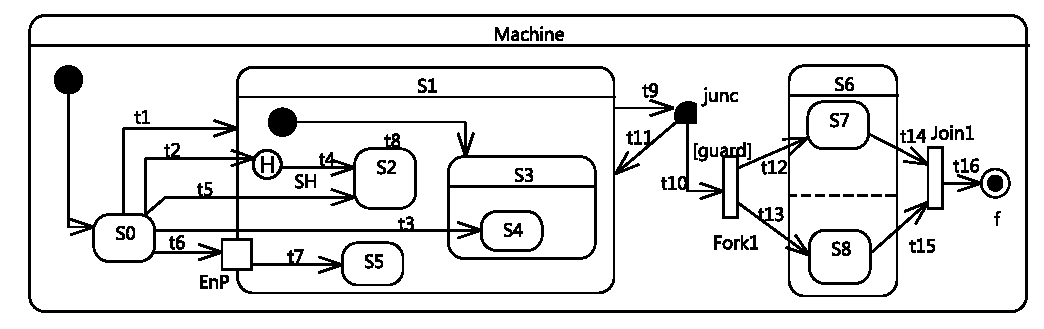
\includegraphics[clip, trim=0.2cm 0.2cm 0.2cm 0.2cm, width=1.0\columnwidth]{figures/EnteringStateExample.pdf}
	\caption{Example illustrating different ways entering a composite state} 
	\label{fig:entering}
\end{figure}

A region $r$ is entered by either a transition $t$ ending at the border of its containing state or on a sub-vertex (direct or indirect), depending on how the state machine is designed. 
The following lists different ways $r$ may be entered:
\begin{itemize}
	\item Way 1: entering by default: $tgt(t) = ctner(r) \wedge src(t) \notin vertices(r)$.
	
	\item Way 2: entering on a direct sub-vertex: $tgt(t) \in vertices(r) \wedge src(t) \notin vertices(r)$.
	
	\item Way 3: entering on an indirect sub-vertex: $ctner(tgt(t)) \in vertices^+(r) \wedge src(t) \notin vertices(r)$.
\end{itemize} 

All of the entering ways execute the entry action of the containing composite state $entry(ctner(r))$ after $effect(t)$. \ti{doActivity(ctner(r))} is then signaled to be run in its associated thread. The actions afterwards are different for each way. To illustrate, we use an example as in Fig. \ref{fig:entering} with \ti{S1} as a target composite state. \ti{t1}, \ti{t3} and \ti{t6} are in the ways of 1 and 3, respectively, while \ti{t2, t5} in the way 2. 

The entering method associated with the region $r$ of \ti{S1} has a parameter $enter\_mode$ indicating how actions should be executed. $enter\_mode$ takes values depending the number of transitions coming to the composite state $S1$: $\#values(s) = \\ \#\{v \in vertices(s)| v.kind=initial\} + \\ \#\{v \in vertices(s)| \exists t \in T_{ins}(v), src(t) \notin vertices(s)\} + \\ 
\#\{v \in vertices^+(s)\setminus vertices(s)|\exists t \in T_{ins}(v), src(t) \notin vertices^+(s)\}$. 
%In this case these values are $\{DEFAULT = 0, SH\_MODE = 1, S2\_MODE = 2, S4\_MODE=3, ENP_MODE=4\}$. 
The detail of how these modes are implemented in specific languages are not discussed here.
Listing \ref{lst:region} shows the C++-like example code generated for $r$.

  
\begin{lstlisting}[caption=Example code generated for the region of S1, label=lst:region]
void S1Region1Enter(int enter_mode){
if (enter_mode == DEFAULT) {
  states[S1_ID].actives[0] = S3_ID;
  states[S3_ID].entry();  sendStartSignal(S3_ID);
  S3Region1Enter(DEFAULT);
} else if (enter_mode == S2_MODE) { 
  //..
} if (enter_mode == SH_MODE) {
  StateIDEnum his;
  if (states[S1_ID].previousActives[0]!=STATE_MAX){
    his = states[S1_ID].previousActives[0];
  } else {
    his = S2_ID;
  }
  states[S1_ID].actives[0] = his;
  states[his].entry();  sendStartSignal(his);
  if (S3_ID == his) {
    S3Region1Enter (S3_REGION1_DEFAULT);
  } 
} else if (enter_mode == S4_MODE) {
  states[S1_ID].actives[0] = S3_ID;
  states[S3_ID].entry();  sendStartSignal(S3_ID);
  S3Region1Enter(S4_MODE);
} else if (enter_mode == ENP_MODE) {...}
\end{lstlisting}




%For each value in $values(s)$, the region of $S1$ is entered and executes different actions. 
By default, the active sub-state of the region is set after the execution of any effect associated with the initial transition, $S3$ is set as active sub-state of $S1$. 
Entering on a direct sub-state (\ti{S2}) sets the active sub-state of \ti{S1} directly to \ti{S2}. 
In case of an indirect sub-state ($S4$), the entry action of $S3$ is executed before $S4$ is set as the active-sub state of $S3$ and the execution of $entry(S4)$. 
It is worth noting that after the execution of each entry, a start signal is sent to activate the waiting thread associated with \ti{doActivity} of the corresponding state.

Transitioning from a vertex to a sub-vertex of the composite state (transition from $S0$ to $SH$ is a particular case) is not as simple as that of two states. It needs a systematic approach which generates code for a transition outgoing from a vertex to any other one. This is detailed in the next section.

\subsection{Event and transition transformation}
\label{subsec:event}
\subsubsection{Events}

Similar to the approach in \cite{niaz_mapping_2004}, one method $mtd_e$ is generated for each event $e$. 
An event enumeration \ti{EventId} is created whose children are event identifiers associated with events. 
%Suppose $levents$ is the list of events which can be processed by the state machine $sm$. 
Besides the explicitly defined events of the state machines, the event list of a state machine $sm$ contains a special event called $CompletionEvent$, which is implicitly implemented as a \ti{CallEvent}. %The latter is, following the UML specification, an implicit event triggering triggerless transitions. It is emitted when either \ti{doActivity} of an atomic state finishes its execution or all regions of a composite state have reached to a final state. 
For each event type, the pattern is realized as in Table \ref{table:event-pattern}.



\begin{table}[]
	\centering
	\caption{Event code generation pattern}
	\label{table:event-pattern}
	\begin{tabular}{p{1.25cm}|p{7.1cm}}
		%\hline
		Event type                                               & Generation pattern                            \\ \hline
		\ti{Call Event} $ce$                                                       & Use The associated operation $op(ce)$ can be either synchronous or asynchronous. When $op(ce)$ is called, it waits and locks the main mutex protecting the run-to-completion semantics, and executes $mtd_{ce}$. Contrarily, the parameters of the asynchronous operation are used to create a signal which is transformed similarly to the case of $SignalEvent$. \\ 
		
		\hline
		
		\ti{Signal Event} $se$                                                       &  $SignalEvent$ is asynchronous. 
		The signal associated with $se$ is written into the event queue of the active class $C$ by an operation which takes as input the signal.                                             \\ 
		
		\hline
		
		\ti{Time Event} $te$                                                     &      A thread $teThread$ associated with $te$ is created and initialized at the initialization of the state machine. 
		Within the execution of $teThread$, the method associated with $te$ waits for a signal, which is sent after the execution of the entry of a state $s \in \{v \in V|\exists t \in T_{outs}(v), te \in events(t)\}$, to start sleeping for a duration $d$ of $te$. 
		When the duration expires, $te$ is emitted and written to the event queue if $s$ is still active.                                         \\ 
		
		\hline
		
		\ti{Change Event} $che$                                                   &                   Similar to $TimeEvent$, a thread $cheThread$ is initialized at initialization but the associated method $mtd$ does not wait for a signal to start. $mtd$ periodically checks whether the value of the associated boolean expression $ex(che)$ changes by comparing the current value with the previous value. 
		If a change happen, $che$ is committed to the event queue.                            \\ 
		
		\hline
		\ti{Any}                                                &        any of the above events can trigger the associated transitions.                                        \\ \hline
	\end{tabular}
\end{table}

\begin{comment}
\begin{itemize}
	\item \ti{CallEvent} $ce$: The associated operation $op(ce)$ can be either synchronous or asynchronous. When $op(ce)$ is called, it waits and locks the main mutex protecting the run-to-completion semantics, and executes $mtd_{ce}$. Contrarily, the parameters of the asynchronous operation are used to create a signal which is transformed similarly to the case of $SignalEvent$.
	
	\item \ti{SignalEvent} $se$: $SignalEvent$ is asynchronous. 
	The signal associated with $se$ is written into the event queue of the active class $C$ by an operation which takes as input the signal. 
	
	\item \ti{TimeEvent} $te$: A thread $teThread$ associated with $te$ is created and initialized at the initialization of the state machine. 
	Within the execution of $teThread$, the method associated $te$ waits for a signal, which is sent after the execution of the entry of a state $s \in \{v \in V|\exists t \in T_{outs}(v), te \in events(t)\}$, to start sleeping for a duration $d$ of $te$. 
	When the duration expires, $te$ is emitted and written to the event queue if $s$ is still active.
	
	\item \ti{ChangeEvent} $che$: Similar to $TimeEvent$, a thread $cheThread$ is initialized at initialization but the associated method $mtd$ does not wait for a signal to start. $mtd$ periodically checks whether the value of the associated boolean expression $ex(che)$ changes by comparing the current value with the previous value. 
	If a change happen, $che$ is committed to the event queue.
	
	\item \ti{Any}: any of the above events can trigger the associated transitions.
\end{itemize}
\end{comment}

As above presented, all asynchronous incoming events are stored in a FIFO priority queue, in which each event type has a configurable priority. $CompletionEvent$ always has the highest priority. Others are equal by default. 
Fig. \ref{fig:eventqueue} shows the generic structure of events stored in the queue.  
Event type, priority, identifier, associated state (\ti{stateId}) and data are specified in the structure. 
The associated state \ti{stateId} is used to define the scope of \ti{Completion Event}s. The event method associated with \ti{Completion Event} executes a check on \ti{stateId} (see Listing \ref{lst:event}, line 1).
The event data contain marshaled\footnote{\url{https://en.wikipedia.org/wiki/Marshalling_(computer_science)}} parameters of \ti{SignalEvent}'s signal or \ti{CallEvent}'s parameters.

\begin{figure}
	\centering
	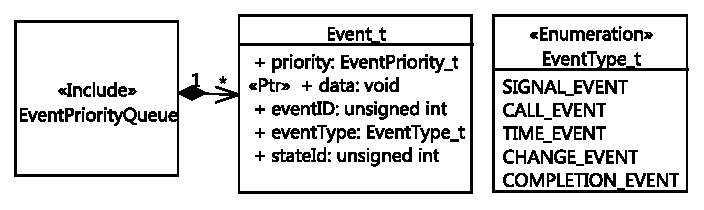
\includegraphics[clip, trim=0.2cm 0.2cm 0.2cm 0.2cm, width=0.6\columnwidth]{figures/eventqueue.pdf}
	\caption{Event data structure} 
	\label{fig:eventqueue}
\end{figure}

\subsubsection{Transitions}

%To process events, for each event, a method is implemented in $C$. 
Each event triggers a list of transitions. We suppose $T_{trig}(e)$ is the transition list triggered by the event $e$, and $S_{trig}(e) = \{src(t) | t \in T_{trig}(e)\}$. In other words, $S_{trig(e)}$ is a set of states which are the source states of the transitions in $T_{trig}(e)$. To present how the body of event methods is generated, we define functions as followings:
\begin{itemize}
	\item Vertex depth $dp(v)$ is defined as:
			\begin{equation}
			dp(v) =    \left\{
			\begin{array}{ll}
			1 & \ti{v is a root vertex}  \\
			dp(ctner(v)) + 1& otherwise \\
			\end{array} 
			\right.
			\end{equation}
	\item $Map_{e}(s) \subset S_{trig(e)} | \forall sub \in Map_e(s): ctner(sub) = s$, $Prt(e) = \{s \in V| Map_{e}(v) \neq \emptyset\}$. $Prt(e)$ is an ordered list whose length is $len(Prt\{e\})$ and elements are accessed by indexes. The order of $Prt(e)$ is defined as:	$\forall i, j \leq len(Prt\{e\})$, 
	\\ if $i < j, dp(Prt(e).get(i)) \geq dp(Prt(e).get(j))$. 	
\end{itemize}

The procedure in Listing \ref{lst:eventproc} describes how the generation process works with an event. 
It first finds the innermost active states which are able to react $e$ by orderly looping over $Lm_e$. 
For each transition outgoing from an innermost state, code for active states and deferral events, guard checking and transition code segments are generated by $GENERATE\_STATE\_EVENT\_CHECK$, $GENERATE\_GUARD(t)$ and \ti{GENTRANS}, respectively. 
If the identifier of $e$ is equal to one of the deferred event list of the corresponding state (not shown in this paper), $GENERATE\_STATE\_EVENT\_CHECK$ generates code, which checks whether the event to be deferred and pushes the event to a deferral event queue managed by the main thread, which also pushes the deferred events back to the main queue once one of the pending events is processed. 

\begin{lstlisting}[mathescape=true, caption=Generation process for an event, label=lst:eventproc, frame=single]
$\forall$ item $\in Lm(e)$
  $\forall s \in Map_e(item)$
    $T_s = \{t \in T_{trig}(e)|src(t) = s\}$
    $\forall t \in T_s$
	    $GENERATE\_STATE\_EVENT\_CHECK(s, t, e)$
	    $GENERATE\_GUARD(t)$
      $GENTRANS(s,t,tgt(t))$  	
\end{lstlisting}



For a transition $t$, $GENERATE\_STATE\_EVENT\_CHECK$ can generate single or multiple active state checking code. 
The latter occurs if $tgt(t)$ is a $join$. 
The detailed discussion on these is not presented due to space limitation. Listing \ref{lst:event}, line 2-3 show a portion of code, with multiple checking, generated for processing \ti{Completion Event} triggering transitions \ti{t14} and \ti{t15} outgoing from \ti{S6} and \ti{S7}, respectively, to \ti{Join1}. 
In addition, the code portion checks the state associated with the current event, which is a completion emitted upon the completion of either \ti{S6}'s or \ti{S7}'s \ti{doActivity}, and saved in the event queue of the active class \ti{C}. 
Lines 4-6 of the portion concurrently exits the sub-states of \ti{S6} by using \ti{FORK} and \ti{JOIN} for methods associated with \ti{S6}'s orthogonal regions, which actually exit ti{S7} and \ti{S8}. Then, \ti{exit(S6)} is executed before the concurrency of transition effects \ti{t14} and \ti{t15} is taken into account.



\begin{lstlisting}[caption=Example code generated for completion events triggering transitions t14 and t15, label=lst:event, language=C++,frame=none]
if(event.stateId==S6_ID||event.stateId==S7_ID){
	if (states[S6_ID].actives[0] == S7_ID && 
		states[S6_ID].actives[1] == S8_ID) {
		thread_r1=FORK(S6Region1Exit); 
		thread_r2=FORK(S6Region2Exit);
		JOIN(thread_r1);  	  JOIN(thread_r2);
		sendStopSignal(S6_ID);  exit_S6();
		thread_t14=FORK(effect(t14));  
		thread_t15=FORK(effect(t15));
		JOIN(thread_t14);  JOIN(thread_t15);
		effect_t16();
		activeStateID = STATE_MAX;  //inactive state
	}
}
\end{lstlisting}
  



\begin{comment}
\begin{algorithm}[]
	\caption{Code generation for transition
		\label{alg:transitiongeneration}}
	\begin{algorithmic}[1]
		\Require{A source $v_{s}$, a target vertex $v_{t}$ and a transition $t$}
		\Ensure{Code generation for transition}
		\Procedure{genTrans}{$v_s$, $v_t$, $t$}
\newline Step 1. Find entry and exit states		
		\State	$H_s$ = $v_s \cup ctner^+(v_s)$, $H_t$ = $v_t \cup ctner^+(v_t)$
		\State {$s_{ex} \in H_s, s_{en} \in H_t | ctner(s_{ex}) = ctner(s_{en})$}
		%\Let{\{$s_{ex}, s_{en}$\}}{$FINDEXE(v_s, v_t)$}
\newline Step 2. Generate IF-ELSE statements for junctions
\newline Step 3. If $s_{ex}$ is a state
		\For {$ r \in regions(s_{ex})$}
		\State {$FORK(RegionExit(r))$}
		\EndFor
		\State {Generate JOIN for threads created above}
		\State {Generate sendStopSignal to $s_{ex}$}
		\State {$exit(s_{ex})$}	
\newline Step 4. If $v_t.kind=join$
		\For {$in \in T_ins(v_t)$}
		\State {$FORK(effect(in))$}
		\EndFor
		\State {Generate JOIN for threads created above}
\newline Step 5. Else
		\State {$effect(t)$}	
\newline Step 7. If $s_{en}$ is a state
		\State {$entry(s_{en})$}
		\State {Generate sendStartSignal to $s_{en}$}
			\newline Step 8. If $s_{en}.kind\in\{conp,conc\}$
				\For {$ r \in regions(s_{en})$}
				\State {$FORK(RegionEnter(r))$}
				\EndFor
		\State {Generate JOIN for threads created above}
		\newline Step 9. Else
		\State {Generate for pseudo states by patterns}
		\EndProcedure	
	\end{algorithmic}
\end{algorithm}
\end{comment}


\begin{comment}
Require{A source $v_{s}$, a target vertex $v_{t}$ and a transition $t$} \\
Ensure{Code generation for transition} \\
Procedure{genTrans}{$v_s$, $v_t$, $t$} \\
\step Find entry and exit states \\		
$H_s$ = $v_s \cup ctner^+(v_s)$, $H_t$ = $v_t \cup ctner^+(v_t)$ \\
$s_{ex} \in H_s, s_{en} \in H_t | ctner(s_{ex}) = ctner(s_{en})$ \\
Step 2. Generate IF-ELSE statements for junctions			\\
\end{comment}



	\begin{table}[]
		\centering
		\caption{Code generation procedure for transition: GENTRANS}
		\label{alg:transitiongeneration}
		\begin{tabular}{p{1cm}p{7cm}}
			\hline
			Input & A source $v_{s}$, a target vertex $v_{t}$ and a transition $t$ \\
			Output & Generated code for transition \\
			\hline
			Step 1 & Find entry and exit states \newline
			$H_s$ = $v_s \cup ctner^+(v_s)$, $H_t$ = $v_t \cup ctner^+(v_t)$ \newline $s_{ex} \in H_s, s_{en} \in H_t | ctner(s_{ex}) = ctner(s_{en})$ \\
			Step 2 & Generate IF-ELSE statements for junctions                           \\
			Step 3 & If $s_{ex}$ is a state       \newline
			         \-\hspace{0.2cm} For {$ r \in regions(s_{ex})$}  \newline 
			         \-\hspace{0.4cm} {$FORK(RegionExit(r))$} \newline
			         \-\hspace{0.2cm} {Generate JOIN for threads created above} \newline
			         \-\hspace{0.2cm} {Generate sendStopSignal to $s_{ex}$} \newline   
			         \-\hspace{0.2cm} {$exit(s_{ex})$}    \\
			Step 4 & If $v_t.kind=join$ \newline
					\-\hspace{0.2cm} For {$in \in T_ins(v_t)$} \newline
					\-\hspace{0.4cm} {$FORK(effect(in))$} \newline
					\-\hspace{0.2cm} {Generate JOIN for threads created above}
					                    \\
			Step 5 & If $v_t.kind \not=join$ \newline   
					\-\hspace{0.2cm} {$effect(t)$}                        \\
			Step 6 & If $s_{en}$ is a state \newline
					\-\hspace{0.2cm}   {$entry(s_{en})$} \newline
					\-\hspace{0.2cm}   {Generate sendStartSignal to $s_{en}$}                     \\
			Step 7 & If $s_{en}.kind\in\{conp,conc\}$ \newline
					\-\hspace{0.2cm} For {$ r \in regions(s_{en})$} \newline
					\-\hspace{0.4cm} {$FORK(RegionEnter(r))$}    \newline
					\-\hspace{0.2cm} {Generate JOIN for threads created above}                      \\
			Step 8 & If $s_{en}.kind\notin\{conp,conc\}$ \newline
					\-\hspace{0.2cm}  {Generate for pseudo states by patterns}  \\
			\hline
			                                                 
		\end{tabular}
	\end{table}



\begin{comment}

\newline Step 3. If $s_{ex}$ is a state
\For {$ r \in regions(s_{ex})$}
\State {$FORK(RegionExit(r))$}
\EndFor
\State {Generate JOIN for threads created above}
\State {Generate sendStopSignal to $s_{ex}$}
\State {$exit(s_{ex})$}	
\newline Step 4. If $v_t.kind=join$
\For {$in \in T_ins(v_t)$}
\State {$FORK(effect(in))$}
\EndFor
\State {Generate JOIN for threads created above}
\newline Step 5. Else
\State {$effect(t)$}	
\newline Step 7. If $s_{en}$ is a state
\State {$entry(s_{en})$}
\State {Generate sendStartSignal to $s_{en}$}
\newline Step 8. If $s_{en}.kind\in\{conp,conc\}$
\For {$ r \in regions(s_{en})$}
\State {$FORK(RegionEnter(r))$}
\EndFor
\State {Generate JOIN for threads created above}
\newline Step 9. Else
\State {Generate for pseudo states by patterns}
\EndProcedure

\begin{algorithm}[]
	\caption{Code generation for transition
		\label{alg:transitiongeneration}}
	\begin{algorithmic}[1]
		\Require{A source $v_{s}$, a target vertex $v_{t}$ and a transition $t$}
		\Ensure{Code generation for transition}
		\Procedure{genTrans}{$v_s$, $v_t$, $t$}
		\Let{$H_s$}{$v_s \cup ctner^+(v_s)$}
		\Let{$H_t$}{$v_t \cup ctner^+(v_t)$}
		\State {$s_{ex} \in H_s, s_{en} \in H_t | ctner(s_{ex}) = ctner(s_{en})$}
		%\Let{\{$s_{ex}, s_{en}$\}}{$FINDEXE(v_s, v_t)$}
		\State {//Generate IF-ELSE statements for junctions}
		\If {$s_{ex}$ is a state}
		\For {$ r \in regions(s_{ex})$}
		\State {$FORK(RegionExit(r))$}
		\EndFor
		\State {//Generate JOIN for threads created above}
		\State {//Generate sendStopSignal to $s_{ex}$}
		\State {$exit(s_{ex})$}	
		\EndIf
		\If {$v_t.kind=join$}
		\For {$in \in T_ins(v_t)$}
		\State {$FORK(effect(in))$}
		\EndFor
		\State {//Generate JOIN for threads created above}
		\Else
		\State {$effect(t)$}	
		\EndIf
		\If {$s_{en}$ is a state}
		\State {$entry(s_{en})$}
		\State {//Generate sendStartSignal to $s_{en}$}
		\If {$s_{en}.kind\in\{conp,conc\}$}
		\For {$ r \in regions(s_{en})$}
		\State {$FORK(RegionEnter(r))$}
		\EndFor
		\State {//Generate JOIN for threads created above}
		\EndIf
		\Else
		\State {//Generate for pseudo states by patterns}
		\EndIf
		\EndProcedure	
	\end{algorithmic}
\end{algorithm}
\end{comment}

 
 

%It generates the code checking for active states respecting the UML semantics in which the innermost states process the incoming event first. To do this, it first looks in the source state list $S_{trig(e)}$ for the innermost states that accept the event triggering its outgoing transitions. If these found states are children of a concurrent state, $genStateCheck$ generates the checking codes run in parallel, which will be described later in \ref{subsubsec:thread}. Otherwise said, sequential code is generated.


\begin{comment}



\begin{algorithm}[]
	\caption{Find states should be exited and entered
		\label{alg:findexit-entry}}
	\begin{algorithmic}[1]
		\Require{A source $v_{s}$ and a target vertex $v_{t}$}
		\Ensure{Vertexes $s_{ex}$, $s_{en}$ to be exited, and entered, respectively}
		\Procedure{findExE}{$v_s$, $v_t$}
			\Let{$H_s$}{$v_s \cup ctner^+(v_s)$}
			\Let{$H_t$}{$v_t \cup ctner^+(v_t)$}
			\State {$s_{ex} \in H_s, s_{en} \in H_t | ctner(s_{ex}) = ctner(s_{en})$}
		\EndProcedure	
	\end{algorithmic}
\end{algorithm}
\end{comment}

\begin{comment}
\begin{itemize}
	\item $join$: Use $GENTRANS$ for $v$'s outgoing transition.
	
	\item $fork$: Use $FORK$ and $JOIN$ for each of outgoing transitions of $v$.
	
	\item $choice$: For each outgoing, an $IF-ELSE$ is generated for the guard of the outgoing together with code generated by $GENTRANS$ (see Listing \ref{lst:event1}).
	
	\item $junction$: As a static version $choice$, a $junction$ is transformed into an attribute $junc_attr$ and evaluated before any action executed in compound transitions (see Listing \ref{lst:event1}). 
	The value of $junc_attr$ is then used to choose the appropriate transition at the place of $junction$.
	
	\item \ti{shallow history}: The identifiers of states to be exited are kept in $pres$ of $IState$. Restoring the active states using the history is exampled as in Listing \ref{lst:region}. The entering method is executed as default mode at the first time the corresponding composite state is entered (see Listing \ref{lst:region}). \ti{pres} is updated with the active state identifier before exiting the region containing the history.
	
	\item \ti{deep history}: Saving and restoring active states are done at all state hierarchy levels from the composite state containing the deep history down to atomic states. Updating \ti{pres} is committed before exiting the region, which is directly or indirectly contained by a parent state, in which a deep history is present.  
	
	\item $enpoint$: If $enpoint$ has no outgoing transition, the corresponding composite state is entered by default. Otherwise said, $GENTRANS$ is called to generate code for the outgoing transition.
	
	\item $expoint$: The code for the unique transition outgoing from $expoint$ is generated by using $GENTRANS$.
	
	\item $terminate$: The code executes the exit action of the innermost active state, the effect of the transition and destroys the state machine object.
\end{itemize}
\end{comment}







\begin{lstlisting}[caption=Example code generated for $Fork1$ and $junc$, label=lst:event1, language=C++,frame=none]
if(activeRootState==S1_ID) {
  junc = 0; //outgoing transition t9 of junc
  if (guard) {junc = 1;}
  //Exit substates of S1 and S1
  effect(t9);
  if(junc==0) {
	  effect(t11);
  } else {
	  effect(t10)
  }
  FORK(effect(t12)); FORK(effect(t3)); 
  //JOIN ... ==> concurrent execution
  //Enter state S6, S7 and S8
}
\end{lstlisting}


Generically, \ti{GENTRANS} generates code for transitions between any vertexes satisfying the constraints described in Section \ref{subsec:background}. Table \ref{alg:transitiongeneration} shows how the transition code generation works. The generated code is bounded by the deferral events, active states, and guard checking.

In the first place, the procedure in Table \ref{alg:transitiongeneration} looks for the composite states $s_{ex}$ and $s_{en}$ at the highest level to be exited and entered (Step 1), respectively. 
If the transition $t$ is part of a compound transition (we use the algorithm presented in \cite{balser2004interactive,Knapp2004} to compute compound transitions), which involves some $junction$s, IF-ELSE statements for junctions are generated first (as PSSM says $junction$ is evaluated before any action). 
The composite state is exited by calling the associated exiting region methods (FORK and JOIN for orthogonal regions) in Step 3 and followed by the generated code of transition effects (Step 4 and 5), respectively. 
If the parent state $s_{en}$ of the target vertex $v_t$ is a state (composite state), the associated entry is executed (Step 6).
Entering region methods are then called once the above code completes its execution (Step 7). 
If the target $v_t$ of the transition $t$ is a pseudo state, the generation pattern corresponding to the pseudo-state types is called. These patterns are shown in Table \ref{table:pseudo-patterm}.

Note that, the procedure in \ref{alg:transitiongeneration} only applies for external transitions. Due to space limitation, the detail of generating local and internal transitions is not discussed here but the only difference is the composite state containing the transitions is not exited.

\begin{table}[]
	\centering
	\caption{Pseudo state code generation pattern}
	\label{table:pseudo-patterm}
	\begin{tabular}{p{1cm}|p{7.3cm}}
		%\hline
		Pseudo state                                               & Code generation pattern                            \\ \hline
		join                                                       & Use $GENTRANS$ for $v$'s outgoing transition (see Listing \ref{lst:event}, lines 4-6). \\ \hline
		fork                                                       &  Use $FORK$ and $JOIN$ for each of outgoing transitions of $v$ (see Listing \ref{lst:event1}, lines 11-12).                                             \\ \hline
		choice                                                     &      For each outgoing, an $IF-ELSE$ is generated for the guard of the outgoing together with code generated by $GENTRANS$.                                         \\ \hline
		junction                                                   &                   As a static version $choice$, a $junction$ is transformed into an attribute $junc_{attr}$ and evaluated before any action executed in compound transitions (see Listing \ref{lst:event1}, lines 2-3 and 6-10). 
		The value of $junc_{attr}$ is then used to choose the appropriate transition at the place of $junction$.                            \\ \hline
		\begin{tabular}[c]{@{}l@{}}shallow \\ history\end{tabular} &                The identifiers of states to be exited are kept in $previousActives$ of $IState$. Restoring the active states using the history is exampled as in Listing \ref{lst:region}. The entering method is executed as default mode at the first time the corresponding composite state is entered (see Listing \ref{lst:region}, lines 9-19). \ti{previousActives} is updated with the active state identifier before exiting the region containing the history.                               \\ \hline
		\begin{tabular}[c]{@{}l@{}}deep \\ history\end{tabular}    &                   Saving and restoring active states are done at all state hierarchy levels from the composite state containing the deep history down to atomic states. Updating \ti{pres} is committed before exiting the region, which is directly or indirectly contained by a parent state, in which a deep history is present.                            \\ \hline
		entry point                                                &        If $enpoint$ has no outgoing transition, the corresponding composite state is entered by default. Otherwise said, $GENTRANS$ is called to generate code for each outgoing transition.                                       \\ \hline
		exit point                                                 &          The code for each transition outgoing from $expoint$ is generated by using $GENTRANS$. If $expoint$ has multiple incoming transitions from orthogonal regions, it is generated as a $join$ to multiple-check the source states of these incomings.                                    \\ \hline
		terminate                                                  &                 The code executes the exit action of the innermost active state, the effect of the transition and destroys the state machine object.                              \\ \hline
	\end{tabular}
\end{table}



\begin{comment}
\subsubsection{Example Code} Listing \ref{lst:event} shows a code segment generated for the processing of $verifyingPIN$. Single checking (line 1) checks whether $Idle$ is the current active state, in which $activeStateID$ is the identifier of the current root active state. The $doActivity$ behavior of $Idle$ is then stopped upon receiving a stop signal. The effect of $t2$, $effect(t3)$ and $effect(t4)$ are then executed after $exit(Idle)$. The execution of $emtry(Verifying)$ then follows the changing of root active state to $Verifying$. $doActivity(Verifying)$ is triggered and followed by concurrently entering the two orthogonal regions of $Verifying$ with appropriate modes.

The discussion of Listing \ref{lst:event1} is similar to Listing \ref{lst:event} except that a multiple checking is executed (line 1-2) instead of a single one. The evaluation for $Junction1$ is executed (line 4) before any other actions (semantic conformance) to decide the decision should be taken (line 10-17). 
\end{comment}
 


 



\section{Experiments report}
\label{sec:exp}

In order to evaluate RAOES, we conducted experiments focusing on different aspects. 
Our research questions are as followings:
\begin{description}[\footnotesize]
	\item[\tb{RQ1}] %A state machine \ttt{sm} is used for generating the front-end code. The latter is reversed engineered to produce another state machine \ttt{sm'}. Are \ttt{sm} and \ttt{sm'} identical? In other words: 
	Whether the front-end code generated from a model with USMs can be used for reconstructing the original model. This question is related to the \ti{GETPUT} law defined in \cite{foster_combinators_2007}.
	
	\item[\tb{RQ2}] The back-end code is used for compilation. 
	Does the runtime execution of the back-end code is semantic-conformant to Precise Semantics for UML State Machines (PSSM)? 
	
	\item[\tb{RQ3}] Runtime performance and memory usage is undoubtedly critical in real-time and embedded systems. Particularly, in event-driven systems, the performance is measured by event processing speed. Does code generated by the presented approach outperform existing approaches and use less memory?
\end{description} 

%\begin{description}
%	Runtime performance and memory usage is undoubtedly critical in real-time and embedded systems. Particularly, in event-driven systems, the performance is measured by event processing speed. Does code generated by the presented approach outperform existing approaches and use less memory?
%\end{description}

In the followings, Subsections \ref{subsec:exp1}, \ref{subsec:exp2}, and \ref{subsec:exp3} report the experimental results for RQ1, RQ2, and RQ3, respectively.

\begin{figure}
	\centering
	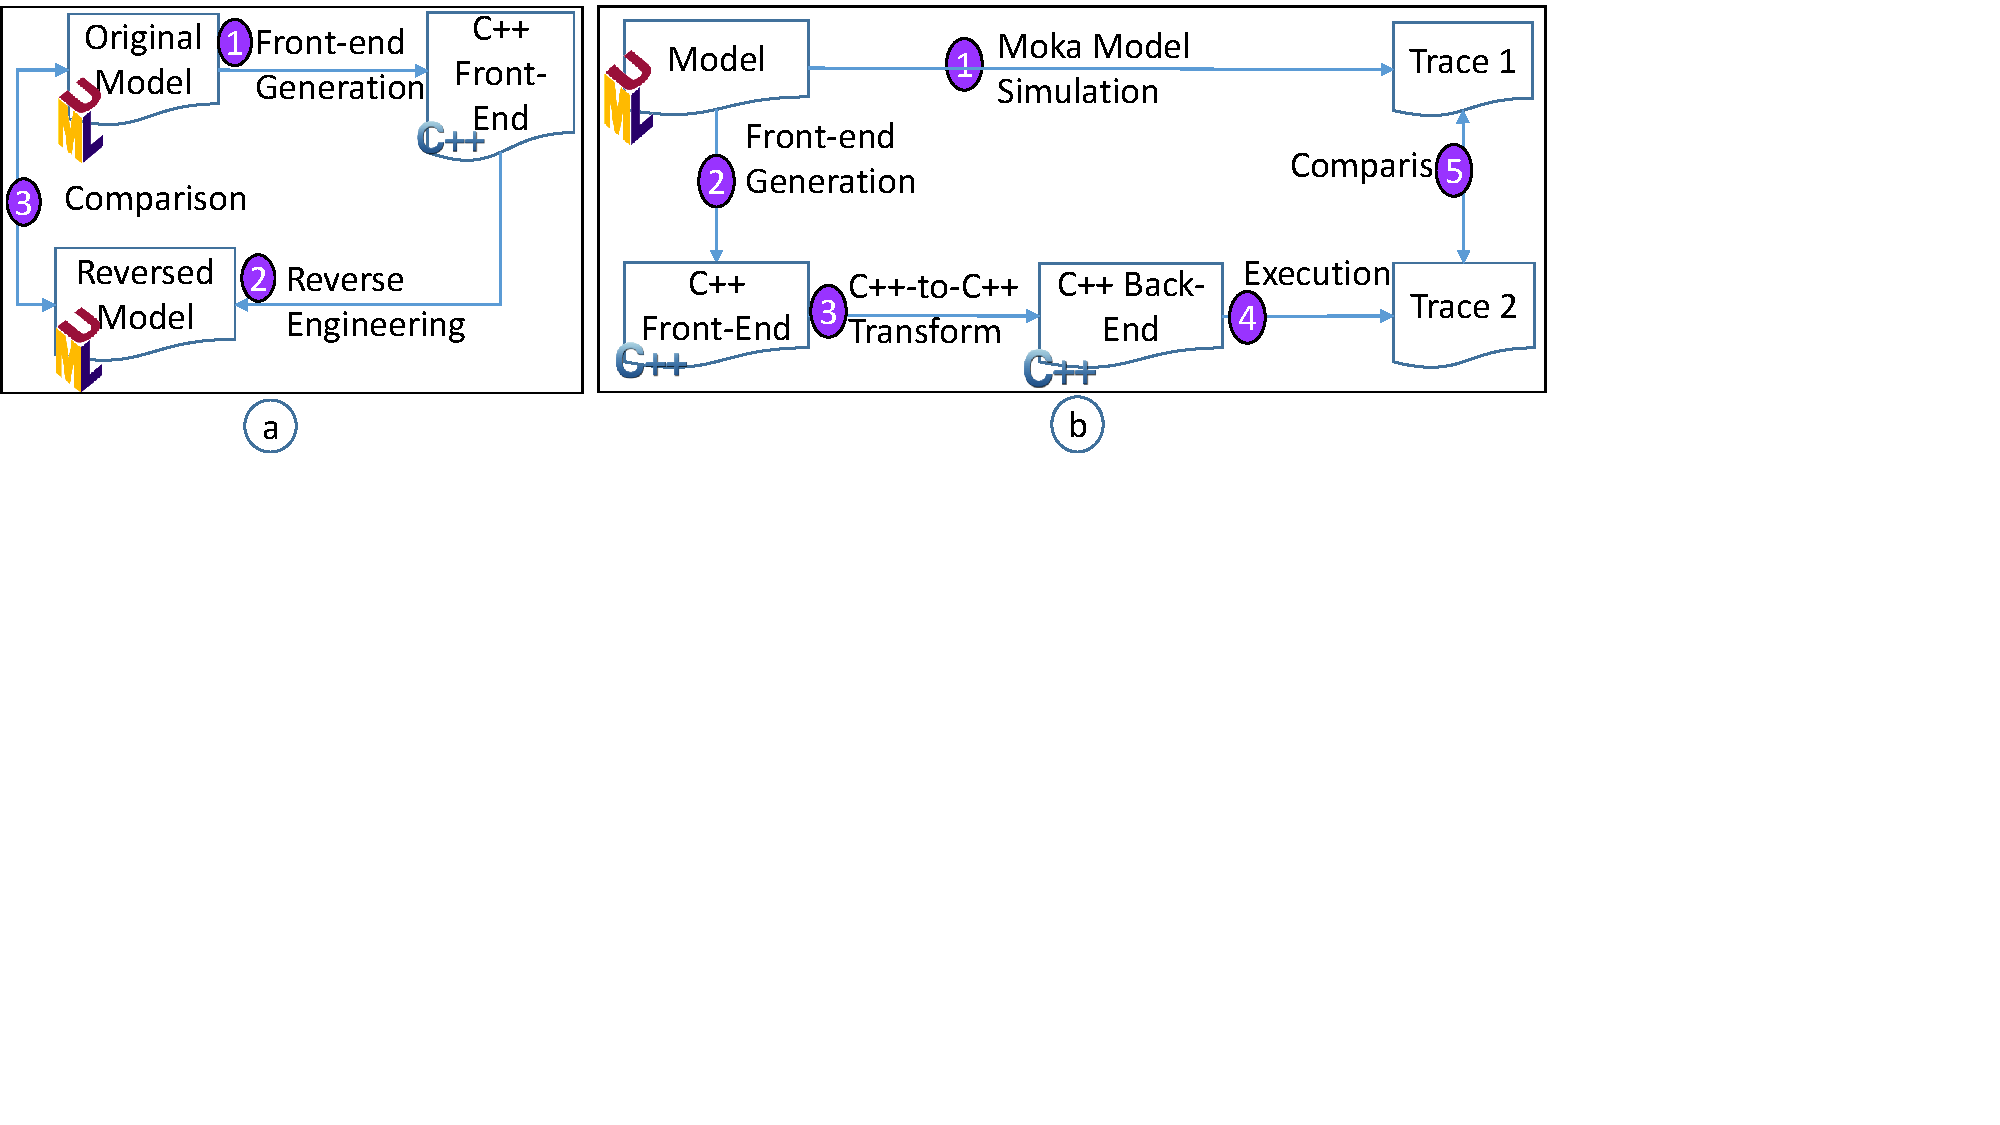
\includegraphics[clip, trim=0cm 11.4cm 7.65cm 0cm, width=\columnwidth]{figures/rq1-2evaluation}
	\caption{Evaluation methodology to answer RQ1 (a) and RQ2 (b)} 
	\label{fig:rq1-2evaluation}
\end{figure}

%\tb{RQ3}: RTE allows developers to freely move between and modify model and code. Specifically, in software development projects, some traditional programmers might want to practice with code in a traditional way and some MDE developers may prefer working with models. What is the development/maintenance cost comparison between the two practices by comparing the number of steps needed to do equivalent actions?

%This section reports our experiments targeting the three questions. Two types of experiments are conducted and presented in Subsections \ref{subsec:exp1} and \ref{subsec:exp2}, respectively. 



\begin{comment}
\begin{figure}
\centering
\includegraphics[clip, trim=5.5cm 19cm 5.5cm 6cm, width=0.3\textwidth]{figures/strategy1}
\caption{Evaluation methodology to answer RQ1} 
\label{fig:strategy1}
\end{figure}

\begin{figure}
\centering
\includegraphics[clip, trim=4.5cm 16.5cm 5.5cm 6.5cm, width=0.3\textwidth]{figures/strategy2}
\caption{Evaluation methodology to answer RQ2} 
\label{fig:strategy2}
\end{figure}
\end{comment}

%Furthermore, in software development projects, some traditional programmers might want to practice with code in a traditional way and some MDE developers may prefer working with models. Therefore, it is necessary to compare the development/maintenance cost between the two practices by comparing the number of steps needed to do the same action. 


\subsection{Reversing generated code}
\label{subsec:exp1}
\tb{RQ1}: A state machine \ttt{sm} is used for generating the front-end code. The latter is reversed engineered to produce another state machine \ttt{sm'}. Are \ttt{sm} and \ttt{sm'} identical? In other words: whether the front-end code generated from USMs model can be used for reconstructing the original model. This question is related to the \ti{GETPUT} law defined in \cite{foster_combinators_2007}.

\begin{figure}
	\centering
	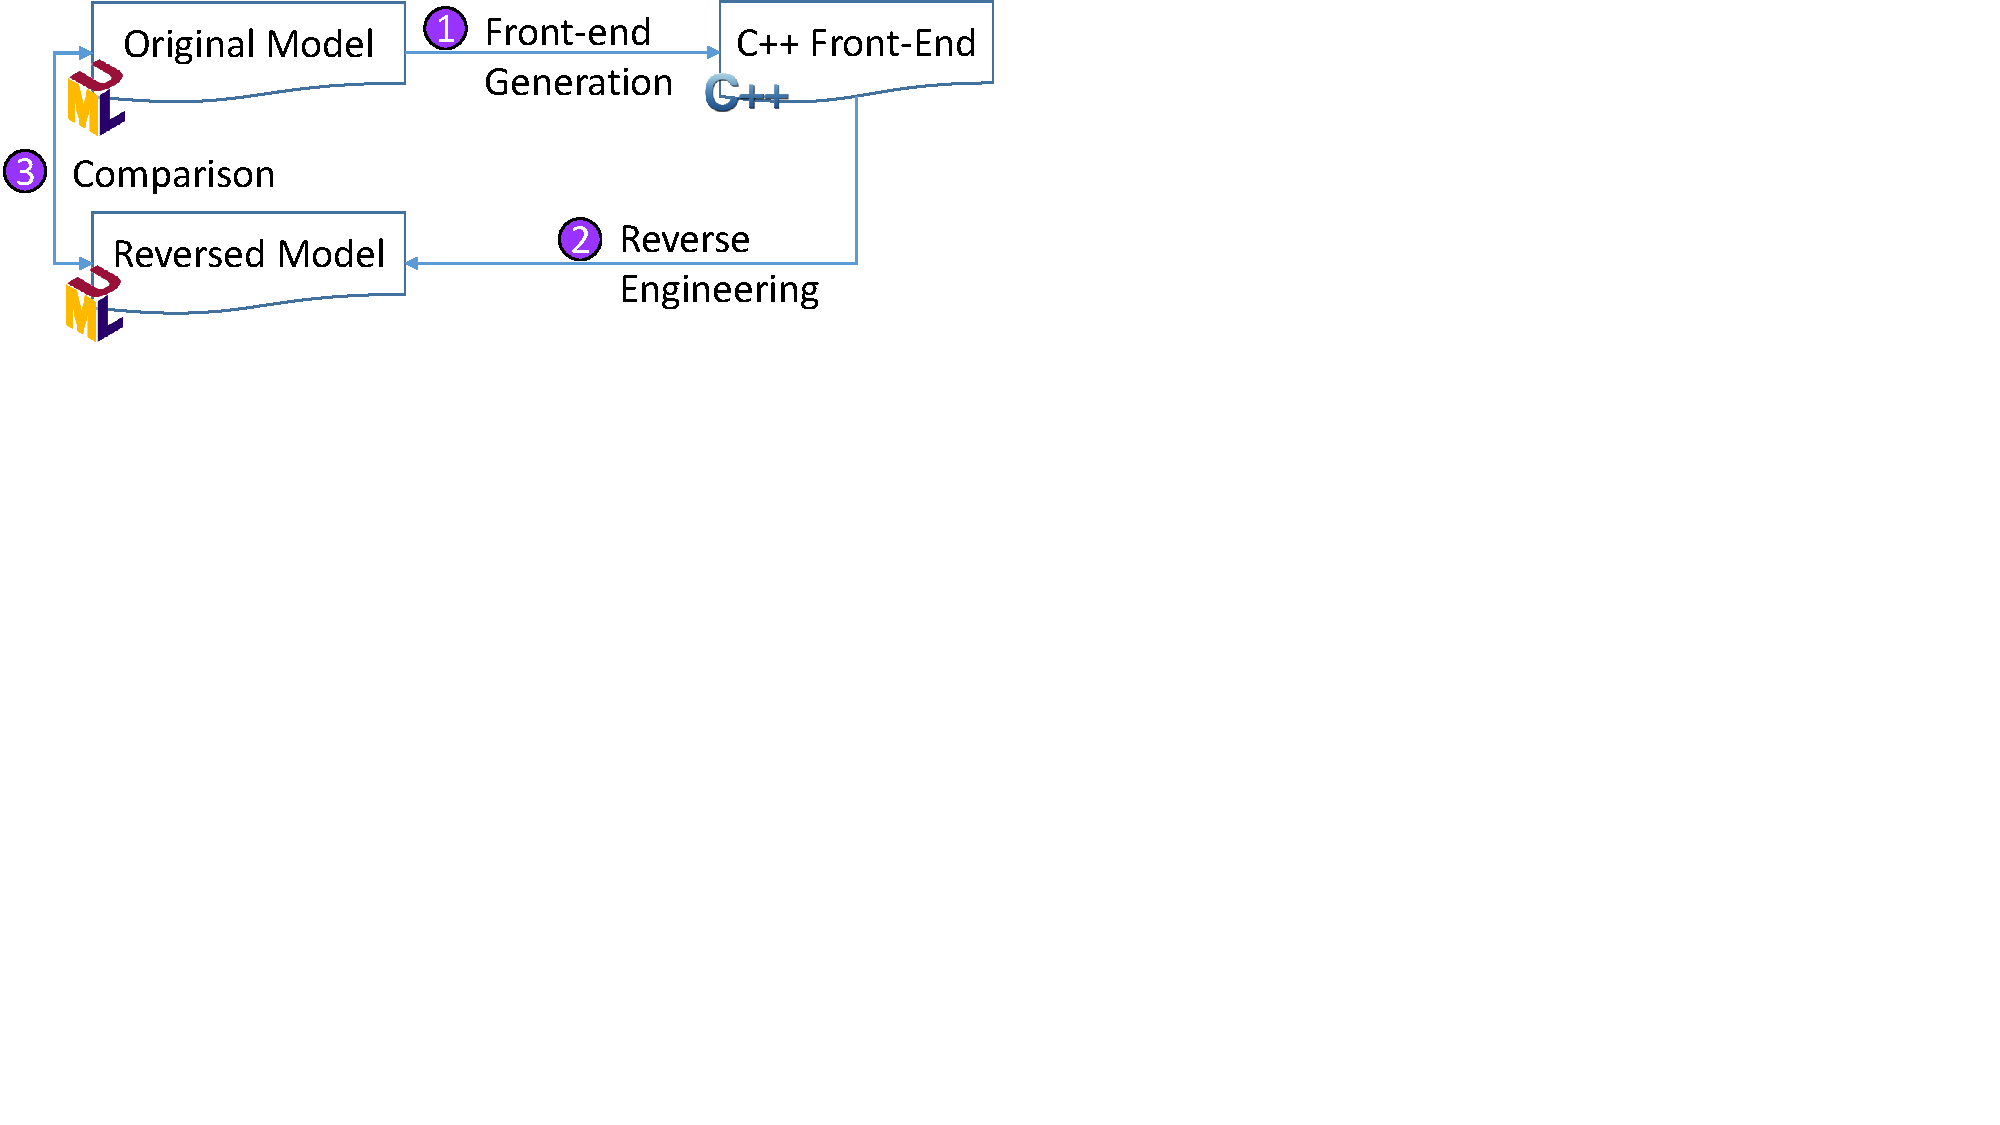
\includegraphics[clip, trim=0cm 13.1cm 16.2cm 0cm, width=\columnwidth]{figures/rteevaluation}
	\caption{Evaluation methodology to answer RQ1} 
	\label{fig:EvaluationStrategyBoth}
\end{figure}

%This experiment is targeting \tb{RQ1}. 
Fig. \ref{fig:EvaluationStrategyBoth} shows the experimental methodology to answer \tb{RQ1}. 
The procedure for this experiment, for each original UML model containing a state machine, consists of 3 steps: 
\begin{description}
	\item[Step 1] \ttt{C++ front-end code} is generated from an \ttt{original model}.
	
	\item[Step 2] The \ttt{C++ front-end code} is reverse engineered to a \ttt{reversed model}
	
	\item[Step 3] The \ttt{reversed model} is then compared to the \ttt{original model}.
\end{description}

%(1) C++ front-end code is generated from an \tb{original model}, (2) the generated code is reverse engineered to a \tb{reversed model}, and (3) the the is then compared to the \tb{original state machine}.% by using information of USM such as the numbers of states and transitions. 

Random models are automatically generated by a configurable model generator. 
The latter can generate a desired average number of vertexes, transitions, and events. 
For each model, a context class and its behavior described by a USM are generated. 
Each USM contains 80 states including atomic and composite states, more than 234 transitions. 
The number of lines of generated C++ code for each machine is around 13500. Names of the generated states are different. 
An initial pseudo state and a final state are generated for each composite state and containing state machine. 
Other elements such as call events, time events, transition/entry/exit actions and guards are generated with a desired configuration. 
For each generated call event, an operation is generated in the context class which is also generated. 
The duration is generated for each time event. 

\begin{comment}
\begin{table}
\centering
\caption{Set-up information for model generation}
\label{table:setup}
\begin{tabular}{|l|l|}
\hline
\rowcolor{Gray}
Description                                     & Value            \\ \hline
%Number of generated states                      & 80               \\ \hline
%Number of generated transitions                 & \textgreater 234 \\ \hline
Probability of having an event for transition   & 0.8              \\ \hline
Probability of having CallEvent for transition  & 0.7              \\ \hline
Probability of having an entry/exit action for state & 0.7              \\ \hline
Probability of having a transition action and guard       & 0.7              \\ \hline
\end{tabular}
\end{table}
\end{comment}

%The set up information for the USM generation is shown in Table \ref{table:setup}. 

\begin{table}
\centering
\caption{Three of model results of generation and reverse: Abbreviations are atomic states (AS), composite states (CS), transitions (T), call events (CE), time events (TE)}
\label{table:law1-resultat}
\begin{tabular}{|l|l|l|l|l|l|l|}
\hline
\rowcolor{Gray}
Test ID & AS & CS & T & CE & TE & Is reverse correct? \\ \hline
1       & 47 & 33 & 234 & 145 & 40 & Yes                 \\ \hline
2       & 42 & 38 & 239 & 145 & 36 & Yes                 \\ \hline
%3       & 43 & 37 & 238 & Yes                 \\ \hline
..      & .. & .. & .. & .. & .. & Yes                 \\ \hline
300       & 41 & 39 &240 & 142 & 37 & Yes                 \\ \hline
\end{tabular}
\end{table}
 
 
\begin{comment}
\begin{table*}[]
\centering
\caption{MODEL RESULTS OF GENERATION AND REVERSE}
\label{table:law1-resultat}
\begin{tabular}{|l|l|l|l|l|l|l|l|l|l|l|l|l|l|}
\hline
\rowcolor{Gray}
Test ID & AS & CS & D  & T   & EA & ExA & TA  & CE  & TE & G   & I  &    & Is reverse correct? \\ \hline
1       & 47 & 33 & 8  & 234 & 53 & 50  & 149 & 145 & 40 & 147 & 34 & 25 & Yes                 \\ \hline
2       & 42 & 38 & 8  & 239 & 52 & 59  & 165 & 145 & 36 & 133 & 39 & 31 & Yes                 \\ \hline
3       & 43 & 37 & 7  & 238 & 54 & 59  & 159 & 141 & 34 & 145 & 38 & 28 & Yes                 \\ \hline
..      & .. & .. & .. & ..  & .. & ..  & ..  & ..  & .. & ..  & .. & .. & Yes                 \\ \hline
300       & 41 & 39 & 10 & 240 & 56 & 55  & 165 & 142 & 37 & 151 & 40 & 33 & Yes                 \\ \hline
\end{tabular}
\end{table*}
\end{comment}

%Table  \ref{table:law1-resultat} shows the number of each type of elements in the randomly generated model, including the comparison results, for 3 of the 200 models created by the generator. We limited ourselves to 200 models for practical reasons

Table \ref{table:law1-resultat} shows the number of several types of elements in the generated models, including the comparison results, for 3 of the 300 models created by the generator. We limited ourselves to 300 models for practical reasons. No differences were found during model comparison. The results of this experiment show that the proposed approach and the implementation can successfully do code generation from state machines and reverse. 

%\input{sections/changepropagation}

%\input{sections/timecomplexity}

%
\subsection{Semantic conformance of runtime execution}
\label{subsec:exp2}
\paragraph{Bisimulation for semantic-conformance}
To evaluate the semantic conformance of runtime execution of generated code, we use a set of examples provided by Moka \cite{moka}. Moka is a model execution engine offering Precise Semantics of UML Composite Structures \cite{OMG2015}. Fig. \ref{fig:semanticconformance} shows our method. We first use our code generator to generate code (Step (1)) from the Moka example set. Step (2) simulates the examples by using Moka to extract the sequence (\ti{SimTraces}) of observed traces including executed actions. The sequence (\ti{RTTraces}) of traces is also obtained by the runtime execution of the code generated from the same state machine in a Step (3). The generated code is semantic-conformant if the sequences of traces are the same for both of the state machine and generated code \cite{Blech2005}. The current version of Moka does not support simulation for \ti{TimeEvent} and history pseudo states, we therefore leave experiments for \ti{TimeEvent} as future work.

For example, Fig. \ref{fig:autotransition} (a) shows a USM example with triggerless transitions (\ti{autotransitions}) \ti{T3}. 
The USM contains two states, \ti{Waiting}, which is the initial state, and \ti{Incrementing}, which increases an integer number from 0 to 5 by using the effect of \ti{T3}. The latter also has a guard checking whether the number is less than 5.
The increase is executed after the USM receives an event named \ti{start} to transition the initial state \ti{Waiting} to \ti{Incrementing}. 
Suppose that executions of the effects of \ti{T3} and \ti{T4} produce traces \ti{<T3>} and \ti{<T4>} (by using MOKA, e.g.), respectively. 
Due to the guard of \ti{T3}, the effect of \ti{T3} is executed five times followed by an execution of the effect of \ti{T4}.
After the completion of the USM, the obtained sequence of traces
is \ti{<T3><T3><T3><T3><T3><T4>} (since the \ti{Incrementing} state does not have an \ti{entry}, \ti{exit}, or a \ti{doActivity}, only the transition effect \ti{T3} produces traces). 
The sequence \ti{RTTraces} obtained by the runtime execution %of the code generated from this USM 
must be equivalent. 
\ti{RTTraces} is obtained by simply printing logging information for each action (effect).

Within our scope as previously defined 30 examples of the Moka example set are tested. \ti{SimTraces} and \ti{RTTraces} for each case are the same. 
This indicates that, within our study scope, the runtime execution of code generated by our generator can produce traces semantically equivalent to those obtained via simulation. 


After experimenting with our code generator, we compare our results to the observed traces obtained by executing code generated 
%by IBM Rhapsody \cite{ibm_rhapsody} and 
Umple \cite{Badreddin2014}. 
We find that the obtained traces in case of 
%IBM Rhapsody and 
Umple are not UML-compliant in triggerless transitions and some cases of event processing.
Specifically, for the example in Fig. \ref{fig:autotransition} (a), 
code generated by Umple only produces \ti{<T3>} as the trace sequence. 
Umple does not support events which are accepted by sub-states and the corresponding composite state as in Fig. \ref{fig:autotransition} (b) in which both \ti{S1} and \ti{S21} accept the event \ti{Continue}.
%Rhapsody does not support self-triggerless transitions as in Fig. \ref{fig:autotransition} and its support for processing events is not totally semantically correct. 
As the processing event example in Fig. \ref{fig:autotransition} (b), assuming that there is an event \ti{Continue} incoming to the state machine which has a current configuration \ti{(S1, S21)} as current active states. While, according to the UML specification, the incoming event should be processed by the inner states of the active composite/concurrent state if the inner states accept it, otherwise the parent state does. Therefore, the next configuration should be \ti{(S1, final state)} and the \ti{T22Effect} effect of the transition \ti{T22} should be executed. %But in case of Rhapsody the next configuration is \ti{End}.   


\begin{figure}
\centering
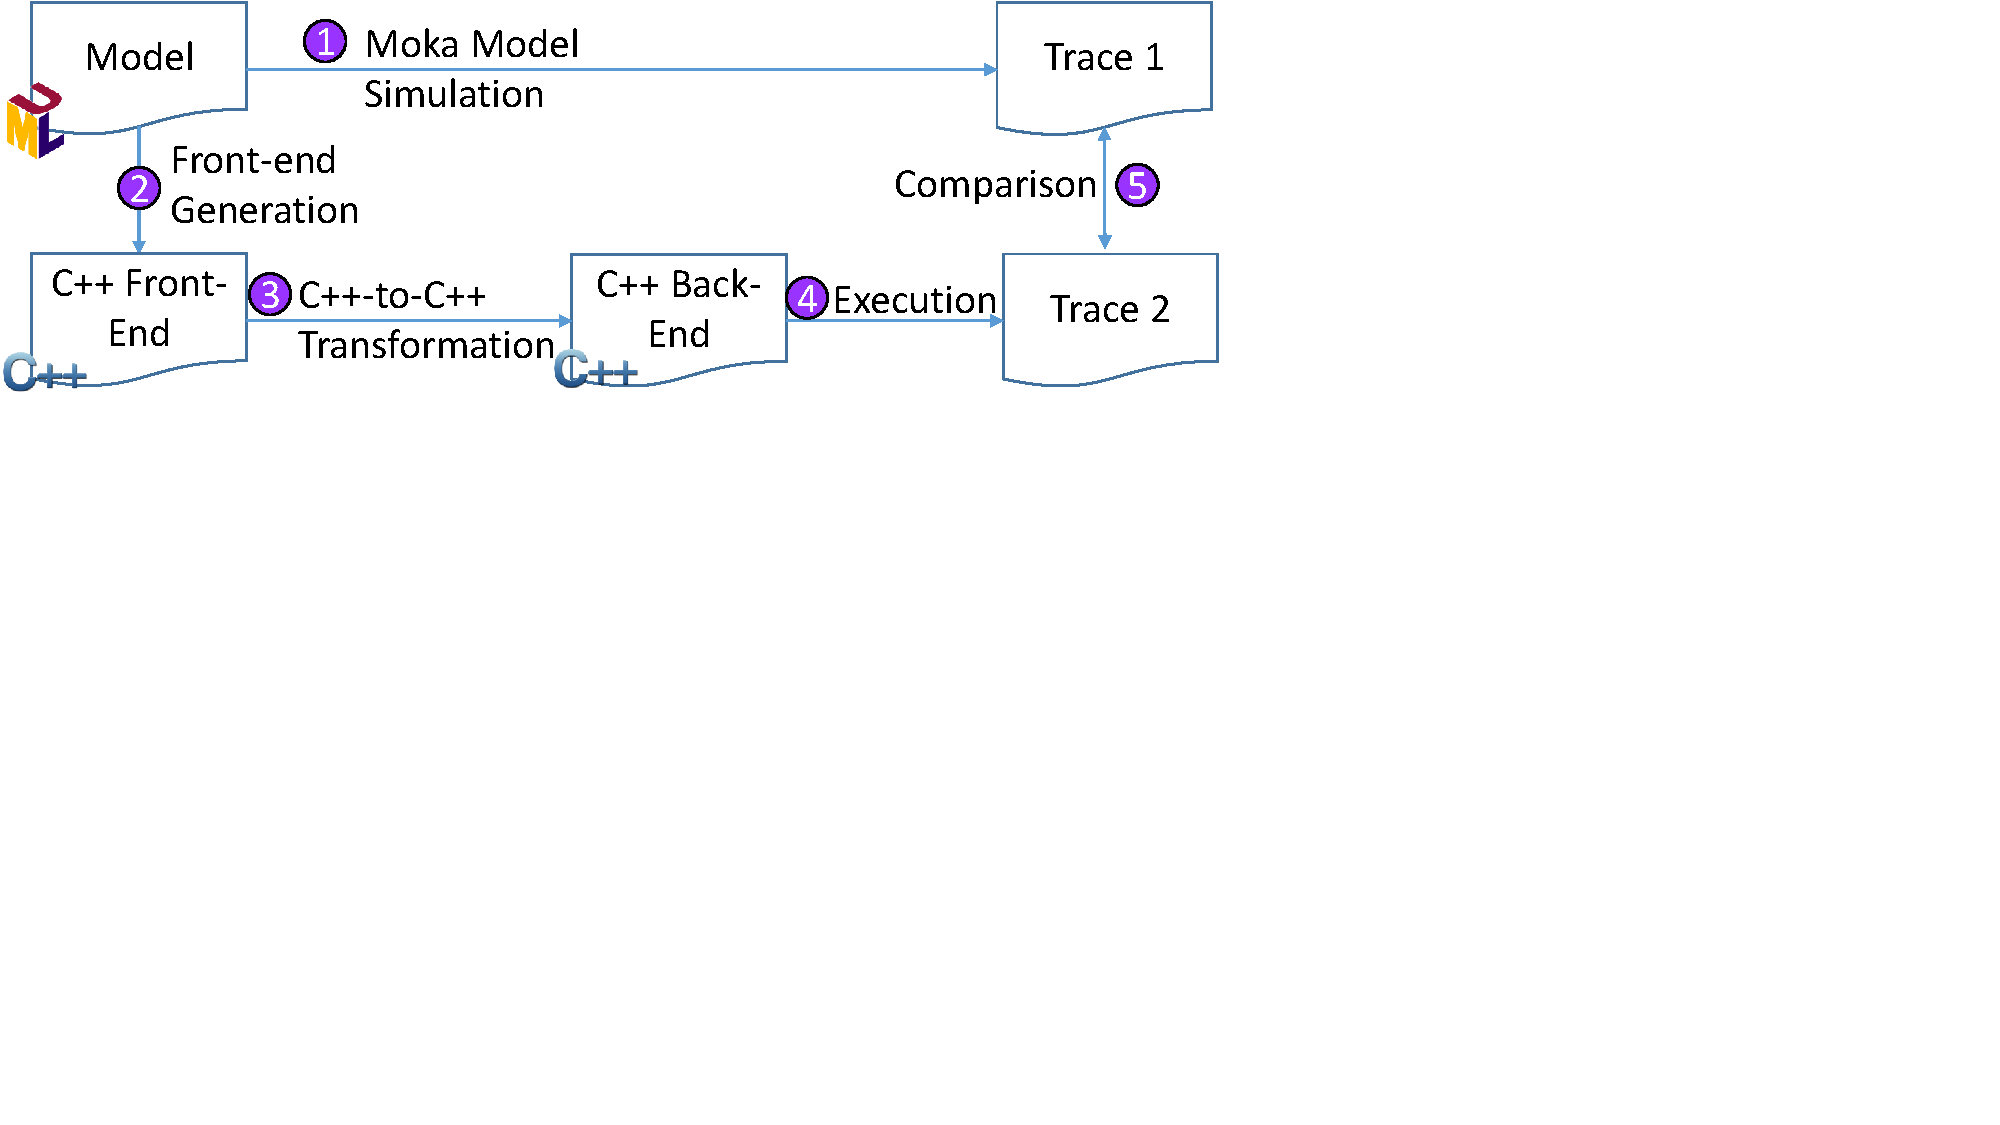
\includegraphics[clip, trim=0.2cm 8.6cm 19.4cm 6.9cm, width=0.8\columnwidth]{figures/semanticconformance.pdf}
\caption{Semantic conformance evaluation methodology} 
\label{fig:semanticconformance}
\end{figure}

\begin{figure}
\centering
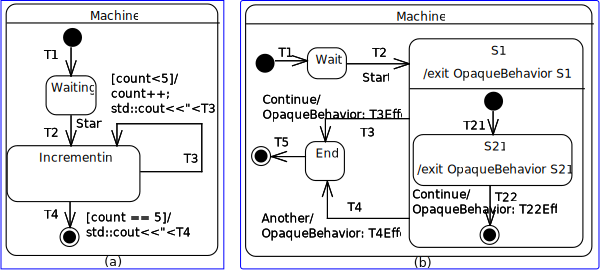
\includegraphics[clip, trim=0cm 0cm 0cm 0cm, width=\columnwidth]{figures/Deferred004Revised}
\caption{Self-triggerless transition and event processing example} 
\label{fig:autotransition}
\end{figure}



\begin{comment}
\begin{figure}
\centering
\includegraphics[clip, trim=0.25cm 0.25cm 0.25cm 0.25cm, width=0.9\columnwidth]{figures/Deferred004}
\caption{Event processing example} 
\label{fig:Deferred}
\end{figure}


\begin{figure*}
\centering
\includegraphics[width=1.5\columnwidth]{figures/ex}
\caption{Self-triggerless transition (a) and event processing (b) examples} 
\label{fig:ex}
\end{figure*}
\end{comment}

\paragraph{Finite state machine}
In addition to the experiment using MOKA, we evaluate the semantic-conformance by using deterministic finite state machines (FSMs). The latter is a mathematical model of computation and also a simplified version of UML state machine. In this experiment, we use FSMs for recognizing input symbols. Each FSM contains many atomic states. The active state of the FSM can be changed following the acceptance of an input symbol. Fig. \ref{fig:fsm} shows our method to experiment. For each FSM, we create an equivalent USM. Each input symbol of the FSM is considered as an event of the USM. We use the FSM simulator in \cite{fsmsim} to generate and simulate FSMs. For each FSM, a list of observed states is recorded as output (\ti{out1}) of the simulation for each symbol list. The latter is also the input of the generated code runtime execution of the equivalent USM which produces an output \ti{out2}. We then compare \ti{out1} and \ti{out2}.

We limit the number of FSMs to 20 and the number of symbol list for each FSM to 30 for practical concerns. 600 sequences of states obtained by the simulation and a same number of sequences taken by the runtime execution are respectively compared and found being equal. This results that our code generation approach can produce semantic-conformant code in case of FSM.

\begin{figure}
	\centering
	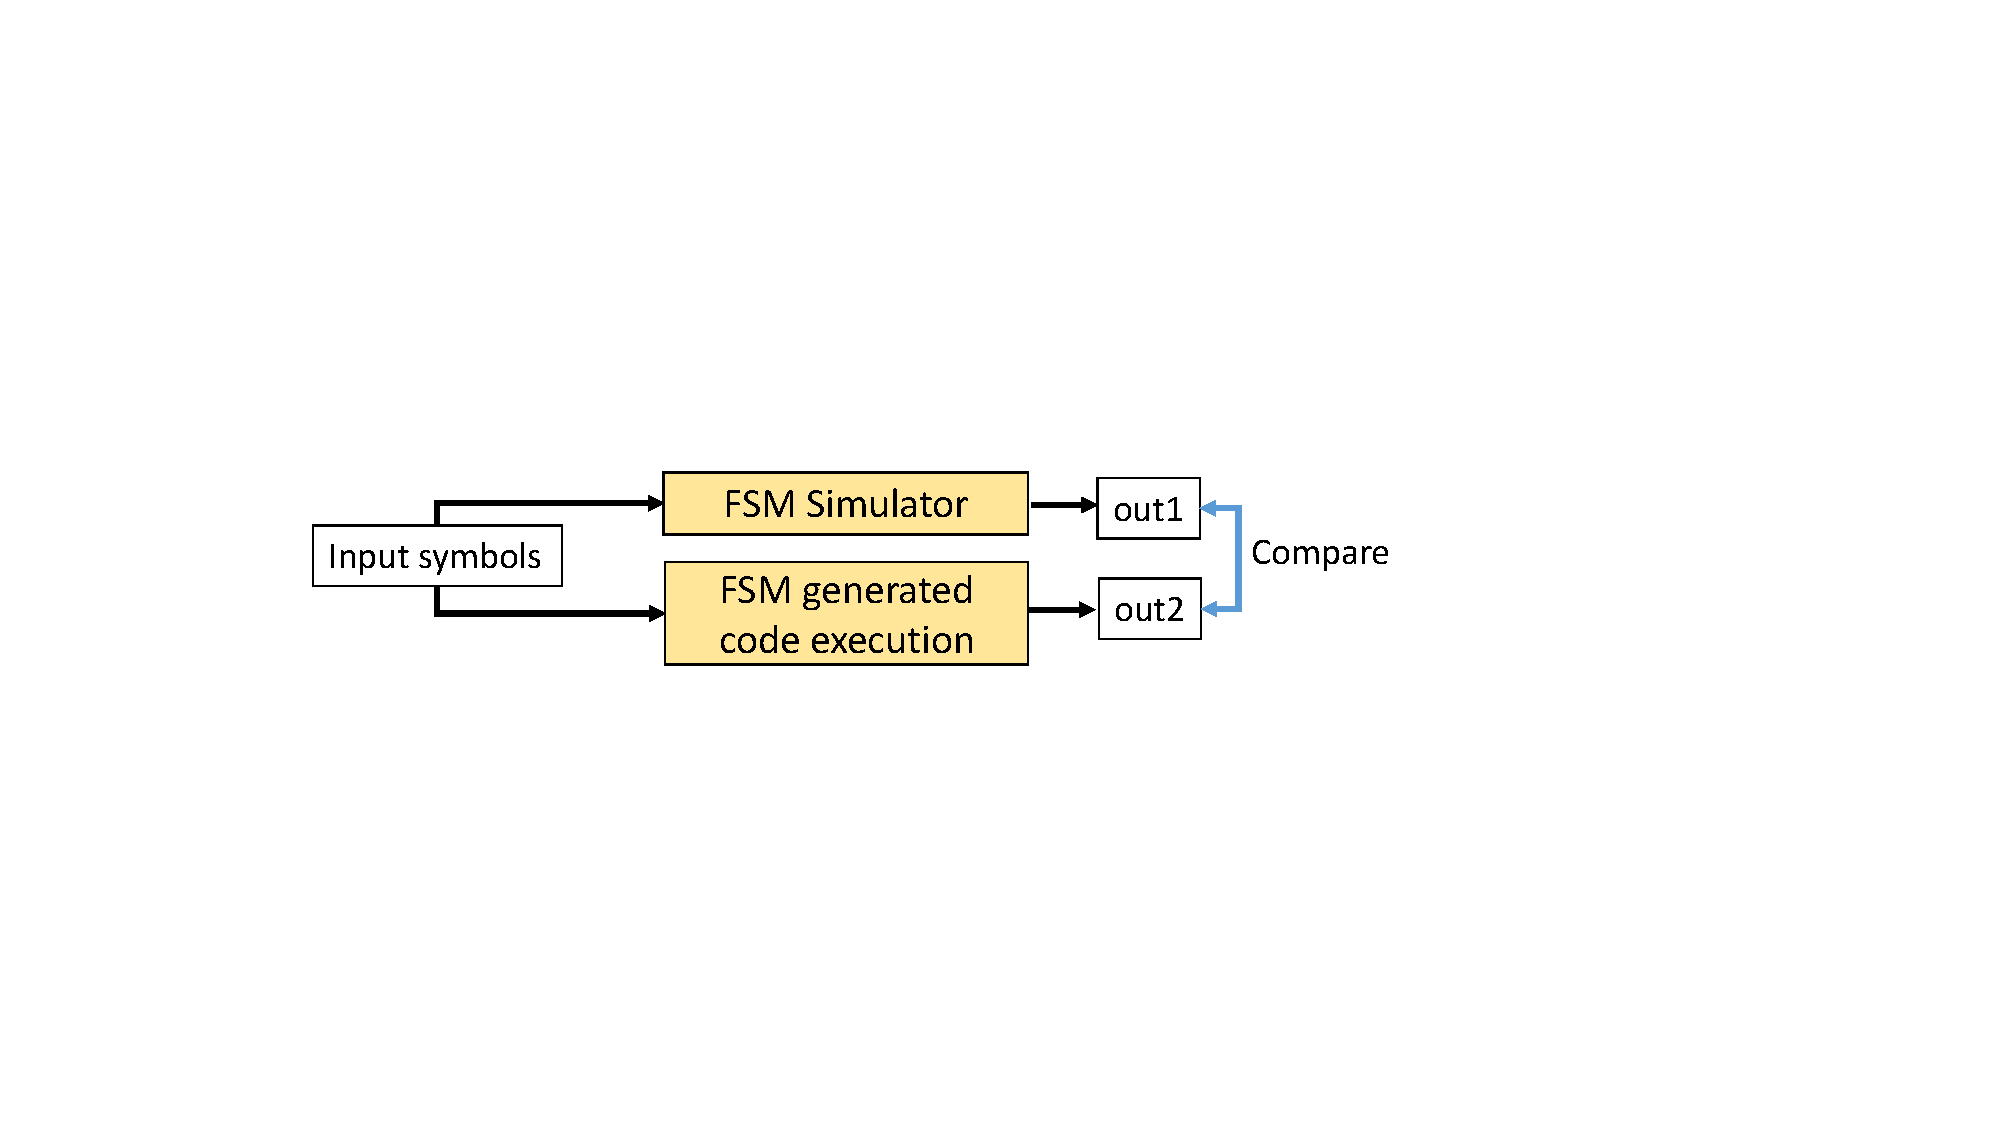
\includegraphics[clip, trim=4.5cm 7.6cm 10.25cm 8.0cm, width=0.85\columnwidth]{figures/fsm}
	\caption{FSM experiment method} 
	\label{fig:fsm}
\end{figure}


%\paragraph{Comparison with IBM Rhapsody}

%\input{sections/developmentcost}

%The approach is implemented as part of the Papyrus Designer tool \cite{qompass} and an extension \tb{PSM} of Papyrus \cite{cea-list_papyrus_????}. This section reports our experiments with \tb{PSM} on the semantic-conformance (Subsection \ref{subsec:exp1}) and efficiency (Subsection \ref{subsec:exp2}) of generated code.

\subsection{Semantic conformance of runtime execution}
\label{subsec:exp2}
%\noindent
%\tb{RQ2:} \ti{The back-end code is used for compilation. Does the runtime execution of the back-end code is semantic-conformant to Precise Semantics for UML State Machines (PSSM)?}.

%\paragraph{Bisimulation for semantic-conformance}
To evaluate the semantic conformance of runtime execution of the back-end code for \tb{RQ2}, we use a set of USM examples provided by \ttt{Moka} \cite{moka}. 
The latter is a model execution engine offering PSSM. 
Fig. \ref{fig:rq1-2evaluation} (b) shows our method, which consists of the following steps:


\begin{description}[\footnotesize]
	\item[Step 1] For a \ttt{model} from the Moka example set, we simulate its execution by using Moka to extract a sequence of traces \ttt{Trace 1}.
	
	\item[Step 2] A \ttt{C++ front-end} code is generated from the \ttt{model} using the front-end generator implemented in Section \ref{subsubsec:gen}.
	
	\item[Step 3] The \ttt{C++ front-end} is used as input for generating a \ttt{C++ back-end} code using the source-to-source transformation.
	
	\item[Step 4] The \ttt{C++ back-end} is compiled for execution to obtain a sequence of traces \ttt{Trace 2}.
	
	\item[Step 5] \ttt{Trace 1} and \ttt{Trace 2} are compared.  
\end{description}

The \ttt{C++ back-end} is semantics-conformant if \ttt{Trace 1} and \ttt{Trace 2} are the same.

%We first use our code generator to generate code (Step (1)) from the Moka example set. Step (2) simulates the examples by using Moka to extract the sequence (\ti{Traces 1}) of observed traces including executed actions. The sequence (\ti{Traces 2}) of traces is obtained by the runtime execution of the code generated from the same state machine in a Step (3). The generated code is semantic-conformant if the sequences of traces are the same for both of the simulation and generated code execution \cite{Blech2005}. %The current version of Moka does not support simulation for \ti{TimeEvent} and history pseudo states, we therefore leave experiments for \ti{TimeEvent} as future work.



%Within our scope as previously defined 30 examples of the Moka example set are tested. \ti{SimTraces} and \ti{RTTraces} for each case are the same. 
%This indicates that, within our study scope, the runtime execution of code generated by our generator can produce traces semantically equivalent to those obtained via simulation. 
PSSM test suite consists of 66 test cases totally for dedicated to different elements.
%Table \ref{table:semantic-test} shows the test results for each state machine concept provided by PSSM. 
The results are promising that RAOES passes 62/66 tests including: behavior (5/6), choice (3/3), deferred events (6/6), entering (5/5), exiting (4/5), entry(5/5), exit (3/3), event (9/9), final state (1/1), fork (2/2), join (2/2), transition (11/14), terminate (3/3), others (2/2).  
In fact, RAOES fails with some wired tests such as transitions from an \ttt{enpoint} to an \ttt{expoint}. 
This is, as our observation, never used in practice. 
Furthermore, as the UML specification says that transitions outgoing from an \ttt{enpoint} of a composite state should end on one of the sub-vertexes.

However, this evaluation methodology has a limitations that it is dependent on PSSM.
Currently, PSSM is not fully defined.
Specifically, only \ttt{SignalEvent} is supported.
On pseudo-states, histories are not supported.
Thus, our evaluation result is limited to the current specification of PSSM.

\begin{comment}
\begin{figure}
	\centering
	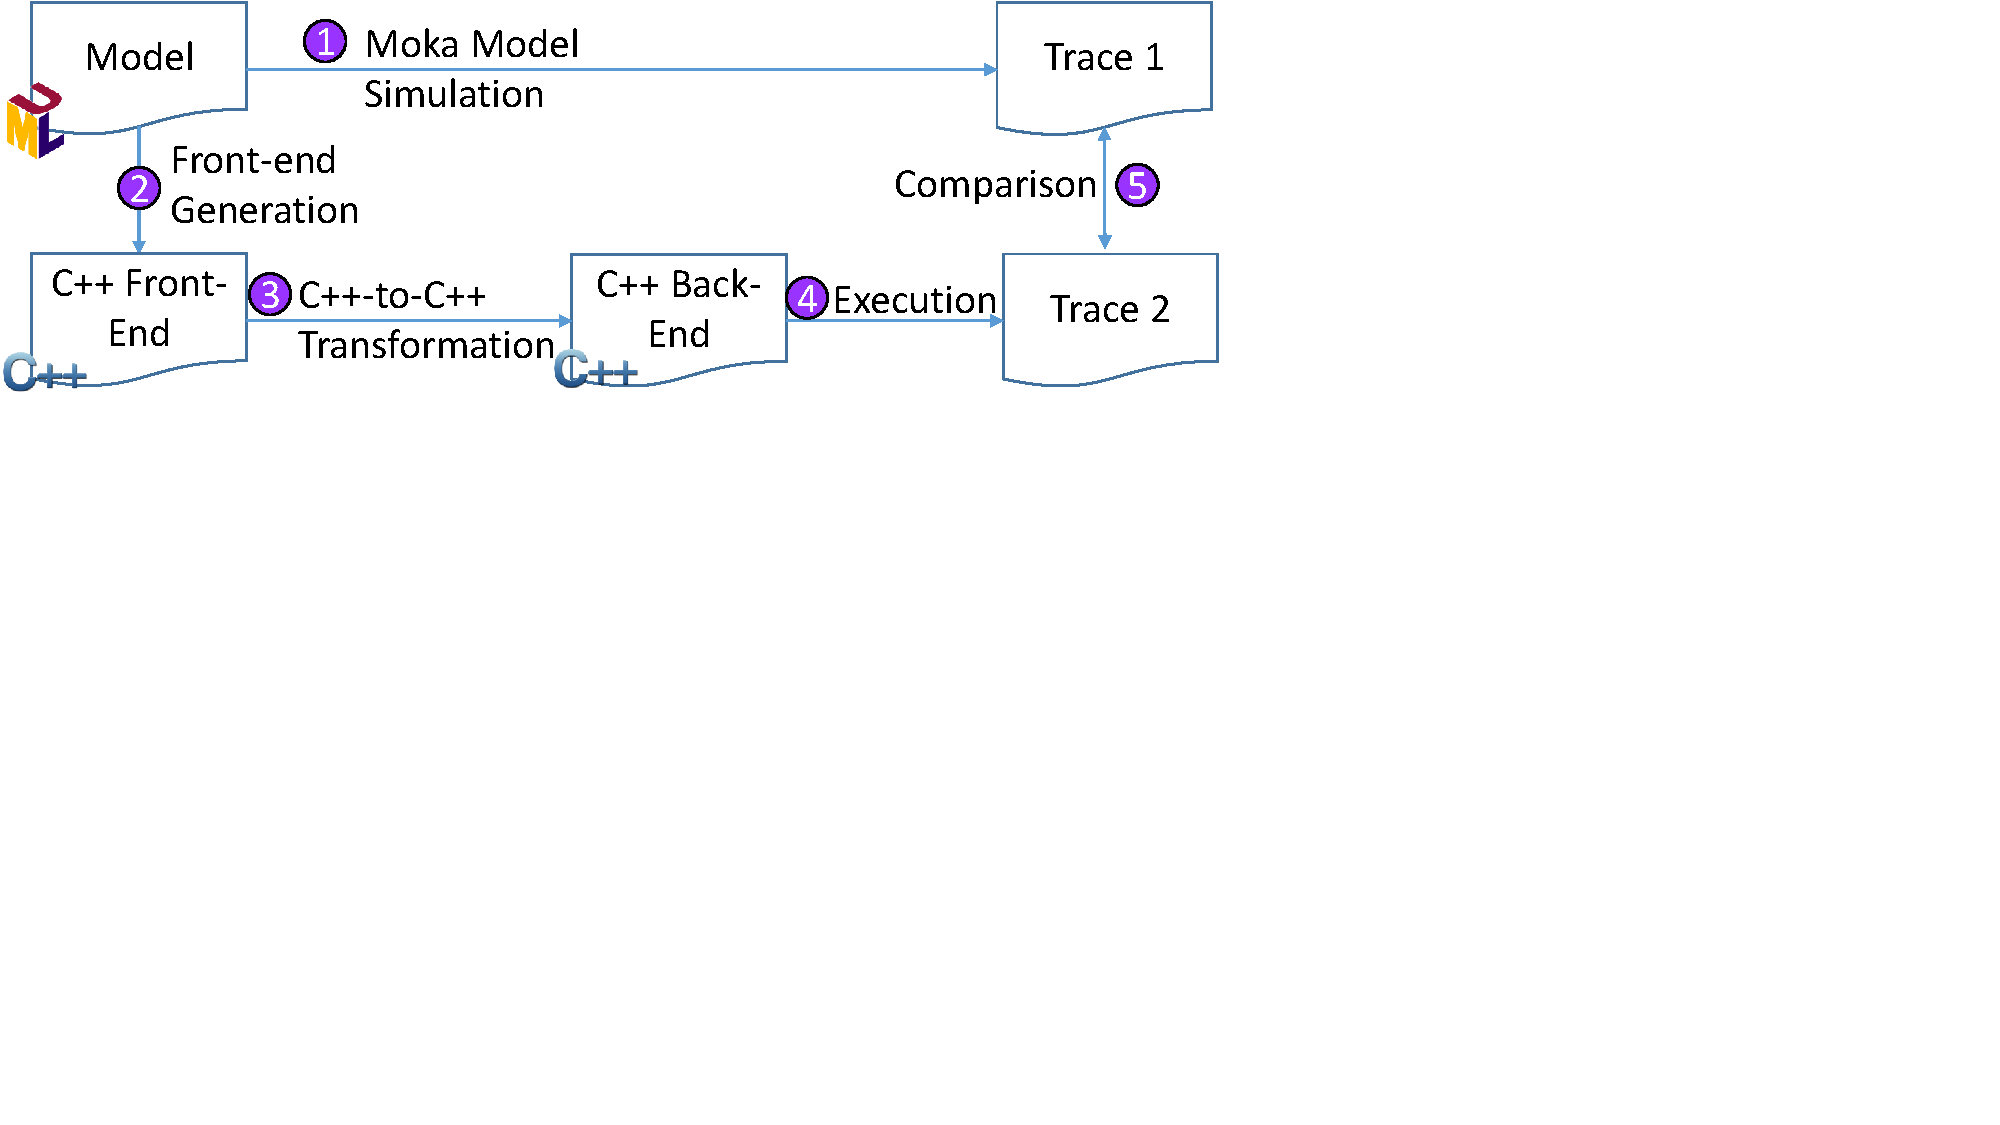
\includegraphics[clip, trim=0cm 12.0cm 12.7cm 0cm, width=\columnwidth]{figures/semanticconformance.pdf}
	\caption{Semantic conformance evaluation methodology} 
	\label{fig:semanticconformance}
\end{figure}		


\begin{table*}[]
	\centering
	\caption{Semantic-conformance test results (number of passed/total tests)}
	\label{table:semantic-test}
	\begin{tabular}{|l|l|l|l|l|l|l|l|l|l|l|l|l|l|}
		\hline
		Behavior & Choice & Deferred Events & Entering & Exiting & Entry & Exit & Event & Final & Fork & Join & Transition & Terminate & Others \\ \hline
		5/6&        3/3&         6/6        &    5/5      &    4/5     &  5/5     &   3/3   &    9/9    &   1/1    &   2/2   &   2/2   &      11/14      &    3/3       &    2/2    \\ \hline
	\end{tabular}
\end{table*}
\end{comment}


%\noindent
%\tb{Threats to validity:}
%Internal threat is that, all test cases of the PSSM test suite are contained in a single model file.
%However, the input to our experiments requires a test case per model file.
%Furthermore, operation behaviors, in PSSM, are defined by activities while our prototype defines behaviors as code blocks embedded into models.
%Therefore, we manually re-create these tests and convert activities into programming language code.

\subsection{Benchmarks}
\label{subsec:exp3}
In this section, we present the results obtained through the experiments on some efficiency aspects of back-end code to answer \tb{RQ3}. 
%Specifically, our research question related to memory consumption and runtime performance of generated code is stated as the following. 

%\noindent
%\tb{RQ3:} \ti{}



%\noindent
%\tb{Experimental dataset:} 
Two state machine examples are obtained by the preferred benchmark used by the Boost C++ libraries \cite{boost} in \cite{benchmark}. One simple example \cite{simpleexample} only consists of atomic states and the other \cite{compositeexample} both atomic and composite states. 

Code generation tools such as Sinelabore (which efficiently generates code for Magic Draw \cite{Magicdraw}, Enterprise Architect \cite{EA}) and QM \cite{qm}
%, which generate code from state machines
, and C++ libraries (Boost Statechart \cite{Statechart}, Meta State Machine (MSM) \cite{MSM}, C++ 14 MSM-Lite \cite{benchmark}, and functional programming like-EUML\cite{EUML}) are used for evaluation. 
%The tools are Sinelabore, which efficiently generates code from UML State Machines created by various modeling tools such as Magic Draw \cite{Magicdraw}, Enterprise Architect \cite{EA}, and QM \cite{QM}. 
%C++ libraries are Boost Statechart \cite{Statechart}, Meta State Machine (MSM) \cite{MSM}, MSM-Lite \cite{MSMLite}, and EUML \cite{euml}.

\noindent
\tb{Experimental procedures:} We use a Ubuntu virtual machine 64 bit (RAM, memory, Ghz??) hosted by a Windows 7 machine. 
For each tool and library, we created two applications corresponding to the two examples, generated C++ code and compiled it two modes: normal (N), by default GCC compiler, and optimal (O) with options -O2 -s. 
11 millions of events are generated and processed by the simple example and more than 4 millions for the composite example. 
%More than 4 millions of events are processed by the composite example. 
Processing time is measured for each case. 

\subsubsection{Speed} 
Fig. \ref{fig:boxplot} shows the event processing performance of the approaches.
%Table \ref{table-speed} shows the median of event processing time. 
In the normal compilation mode (N), Boost Statechart, MSM, MSMLite, EUML are quite slow and not displayed in the box-plot. 
Only Sinelabore and QM are performantly comparable with our approach. 
The table also shows that the optimization of GCC is significant. 
MSM and MSMLite run faster than Sinelabore and QM.   
%Boxplots in Fig. \ref{fig:boxplotsimple} and \ref{fig:boxplotcomposite} compare the performance of these approaches to that of our approach for the two examples, respectively. 
%In both of the simple and composite examples, 

Our approach processes faster around 40 milliseconds than the fastest approach within the scope of the experiment.
It is seen that, even without GCC optimizations, code generated by our approach significantly runs faster than that of EUML and QM with the optimizations. 
When compiled with the optimizations, our approach improves the event processing speed. 
Even, in case of composite, our approach does not produce any slowness compared to the simple example. 


% Please add the following required packages to your document preamble:
% \usepackage{multirow}
\begin{comment}
\begin{table*}[]
	\centering
	\caption{Event processing speed in ms}
\label{my-label}
\begin{tabular}{|l|l|l|l|l|l|l|l|l|l|l|l|l|l|l|l|l|}
	\hline
	\multicolumn{1}{|c|}{\multirow{2}{*}{Test}} & \multicolumn{2}{c|}{SC} & \multicolumn{2}{c|}{MSM} & \multicolumn{2}{c|}{MSM-Lite} & \multicolumn{2}{c|}{EUML} & \multicolumn{2}{c|}{Sinelabore} & \multicolumn{2}{c|}{QM} & \multicolumn{2}{l|}{Umple} & \multicolumn{2}{c|}{Our approach} \\ \cline{2-17} 
	\multicolumn{1}{|c|}{}                      & N           & O         & N            & O         & N              & O            & N            & O          & N               & O             & N          & O          & N            & O           & N                & O              \\ \hline
	Simple                                      & 13705,75    & 1658,1    & 5249,57      & 70,63     & 833,67         & 79,37        & 10867,93     & 109,97     & 141,03          & 79,93         & 285,9      & 229,27     & X            & X           & 106,87           & 25,37          \\ \hline
	Composite                                   & 5353,03     & 820,63    & 3546,1       & 46,73     & 516,87         & 65,17        & 4225,57      & 92,3       & 100,03          & 86,03         & 146,23     & 97,57      & X            & X           & 36,47            & 1,40           \\ \hline
\end{tabular}
\end{table*}
\end{comment}

\begin{comment}
\begin{table*}[]
	\centering
	\caption{Event processing speed in ms}
	\label{table-speed}
	\begin{tabular}{|l|l|l|l|l|l|l|l|l|l|l|l|l|l|l|l|l|}
		\hline
		\multicolumn{1}{|c|}{\multirow{2}{*}{Test}} & \multicolumn{2}{c|}{SC} & \multicolumn{2}{c|}{MSM} & \multicolumn{2}{c|}{MSM-Lite} & \multicolumn{2}{c|}{EUML} & \multicolumn{2}{c|}{Sinelabore} & \multicolumn{2}{c|}{QM} & \multicolumn{2}{l|}{Umple} & \multicolumn{2}{c|}{Our approach} \\ \cline{2-17} 
		\multicolumn{1}{|c|}{}                      & N           & O         & N            & O         & N              & O            & N            & O          & N               & O             & N          & O          & N            & O           & N                & O              \\ \hline
		Simple                                      & 13706    & 1658    & 5250      & 71     & 834         & 79        & 10868     & 110     & 141          & 80         & 286      & 229     & X            & X           & 107           & 25,4          \\ \hline
		Composite                                   & 5353     & 821    & 3546       & 47     & 517         & 65        & 4225,6      & 92       & 100          & 86         & 146     & 98      & X            & X           & 36,5            & 1,40           \\ \hline
	\end{tabular}
\end{table*}
\end{comment}


\begin{comment}
\begin{table*}[]
	\centering
	\caption{Event processing speed in ms}
	\label{table-speed}
	\begin{tabular}{|l|l|l|l|l|l|l|l|l|l|l|l|l|l|l|}
		\hline
		\multicolumn{1}{|c|}{\multirow{2}{*}{Test}} & \multicolumn{2}{c|}{SC} & \multicolumn{2}{c|}{MSM} & \multicolumn{2}{c|}{MSM-Lite} & \multicolumn{2}{c|}{EUML} & \multicolumn{2}{c|}{Sinelabore} & \multicolumn{2}{c|}{QM} & \multicolumn{2}{c|}{PSM} \\ \cline{2-15} 
		\multicolumn{1}{|c|}{}                      & N           & O         & N            & O         & N              & O            & N             & O         & N               & O             & N          & O          & N           & O          \\ \hline
		Simple                                      & 13706       & 1658      & 5250         & 71        & 834            & 79           & 10868         & 110       & 141             & 80            & 286        & 229        & 107         & 25,4       \\ \hline
		Composite                                   & 5353        & 821       & 3546         & 47        & 517            & 65           & 4225,6        & 92        & 100             & 86            & 146        & 98         & 36,5        & 1,40       \\ \hline
	\end{tabular}
\end{table*}
\end{coment}


\begin{comment}
\begin{figure}
	\centering
	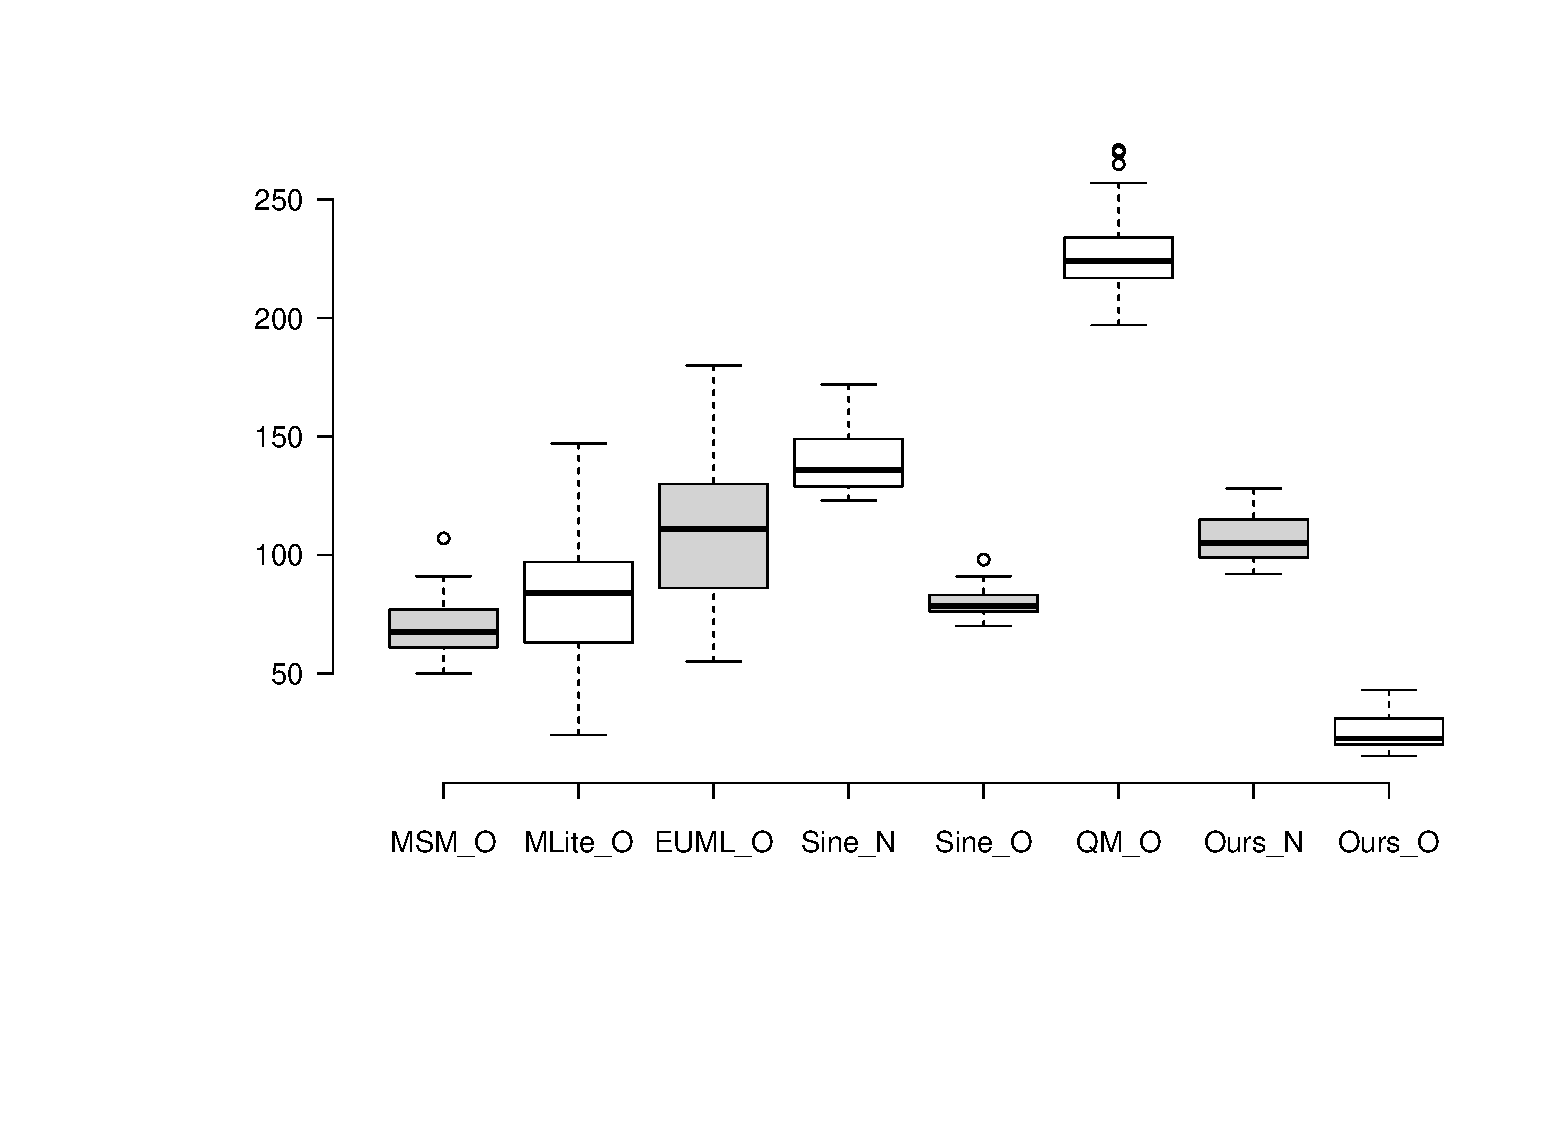
\includegraphics[clip, trim=4.2cm 4.6cm 1.7cm 2.3cm, width=\columnwidth]{figures/boxplotsimple.pdf}
	\caption{Event processing speed for the \ti{Simple} benchmark} 
	\label{fig:boxplotsimple}
\end{figure}

\begin{figure}
	\centering
	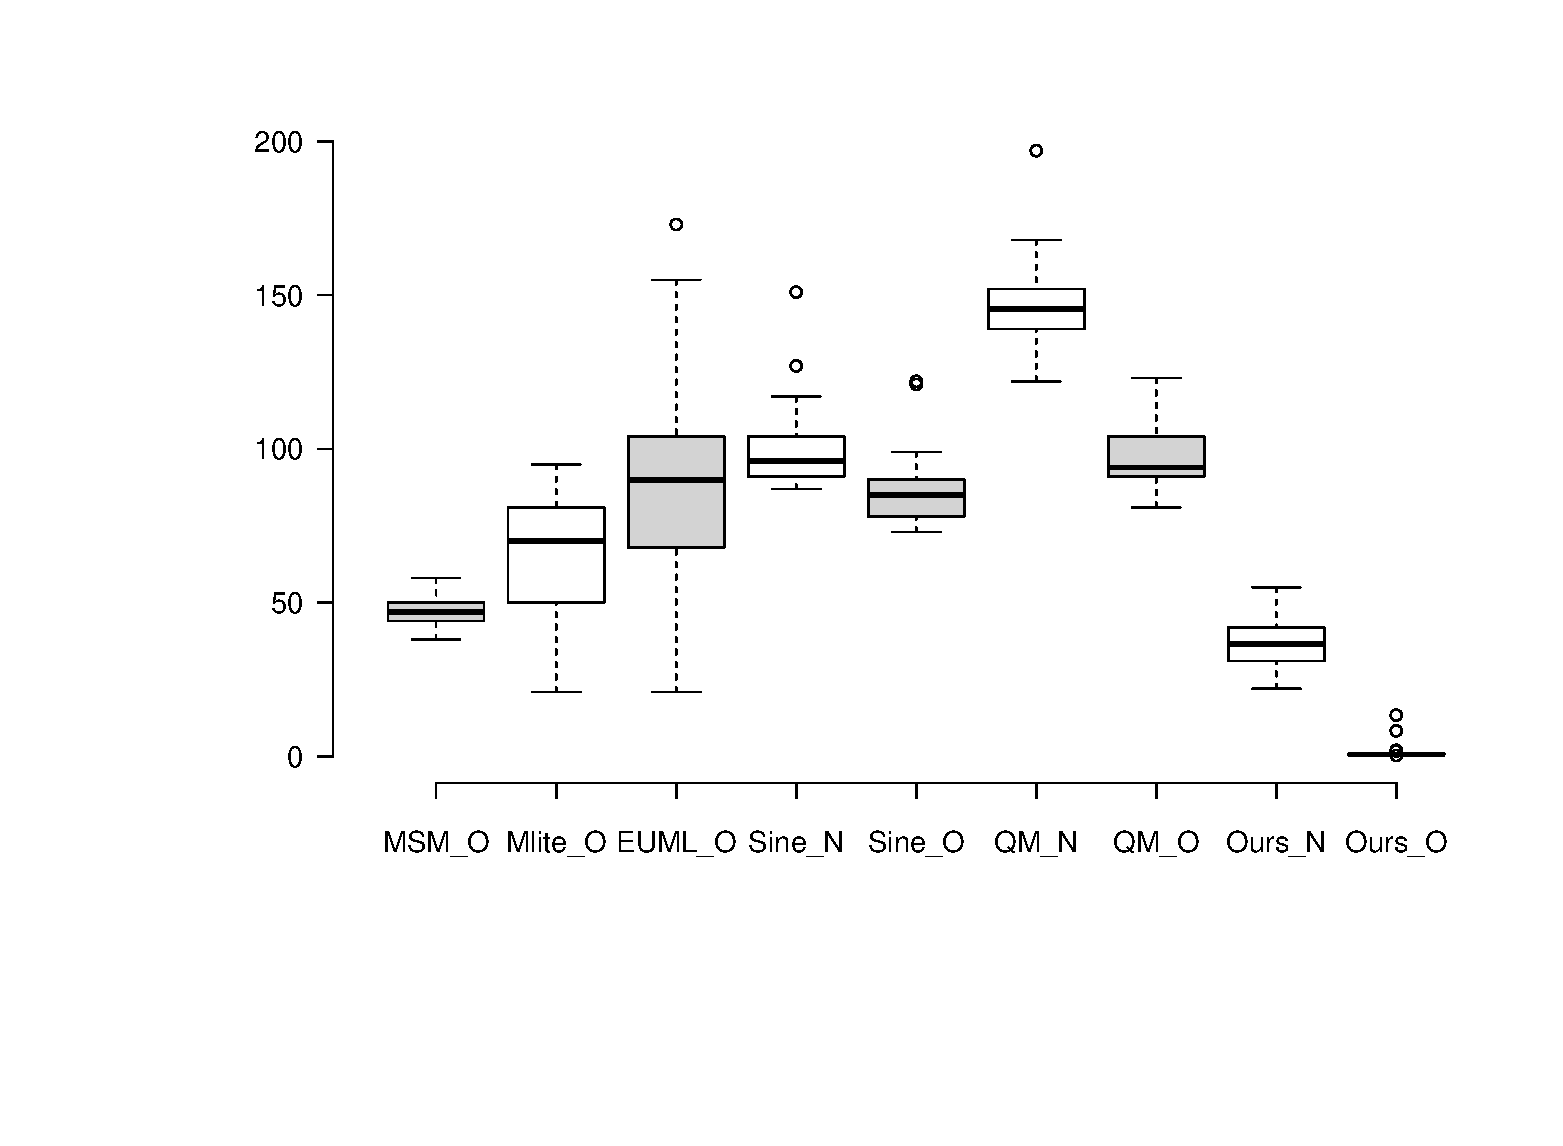
\includegraphics[clip, trim=4.2cm 4.6cm 1.7cm 1.8cm, width=\columnwidth]{figures/boxplotcomposite.pdf}
	\caption{Event processing speed for the \ti{Composite} benchmark} 
	\label{fig:boxplotcomposite}
\end{figure}
\end{comment}

\begin{figure}
	\centering
	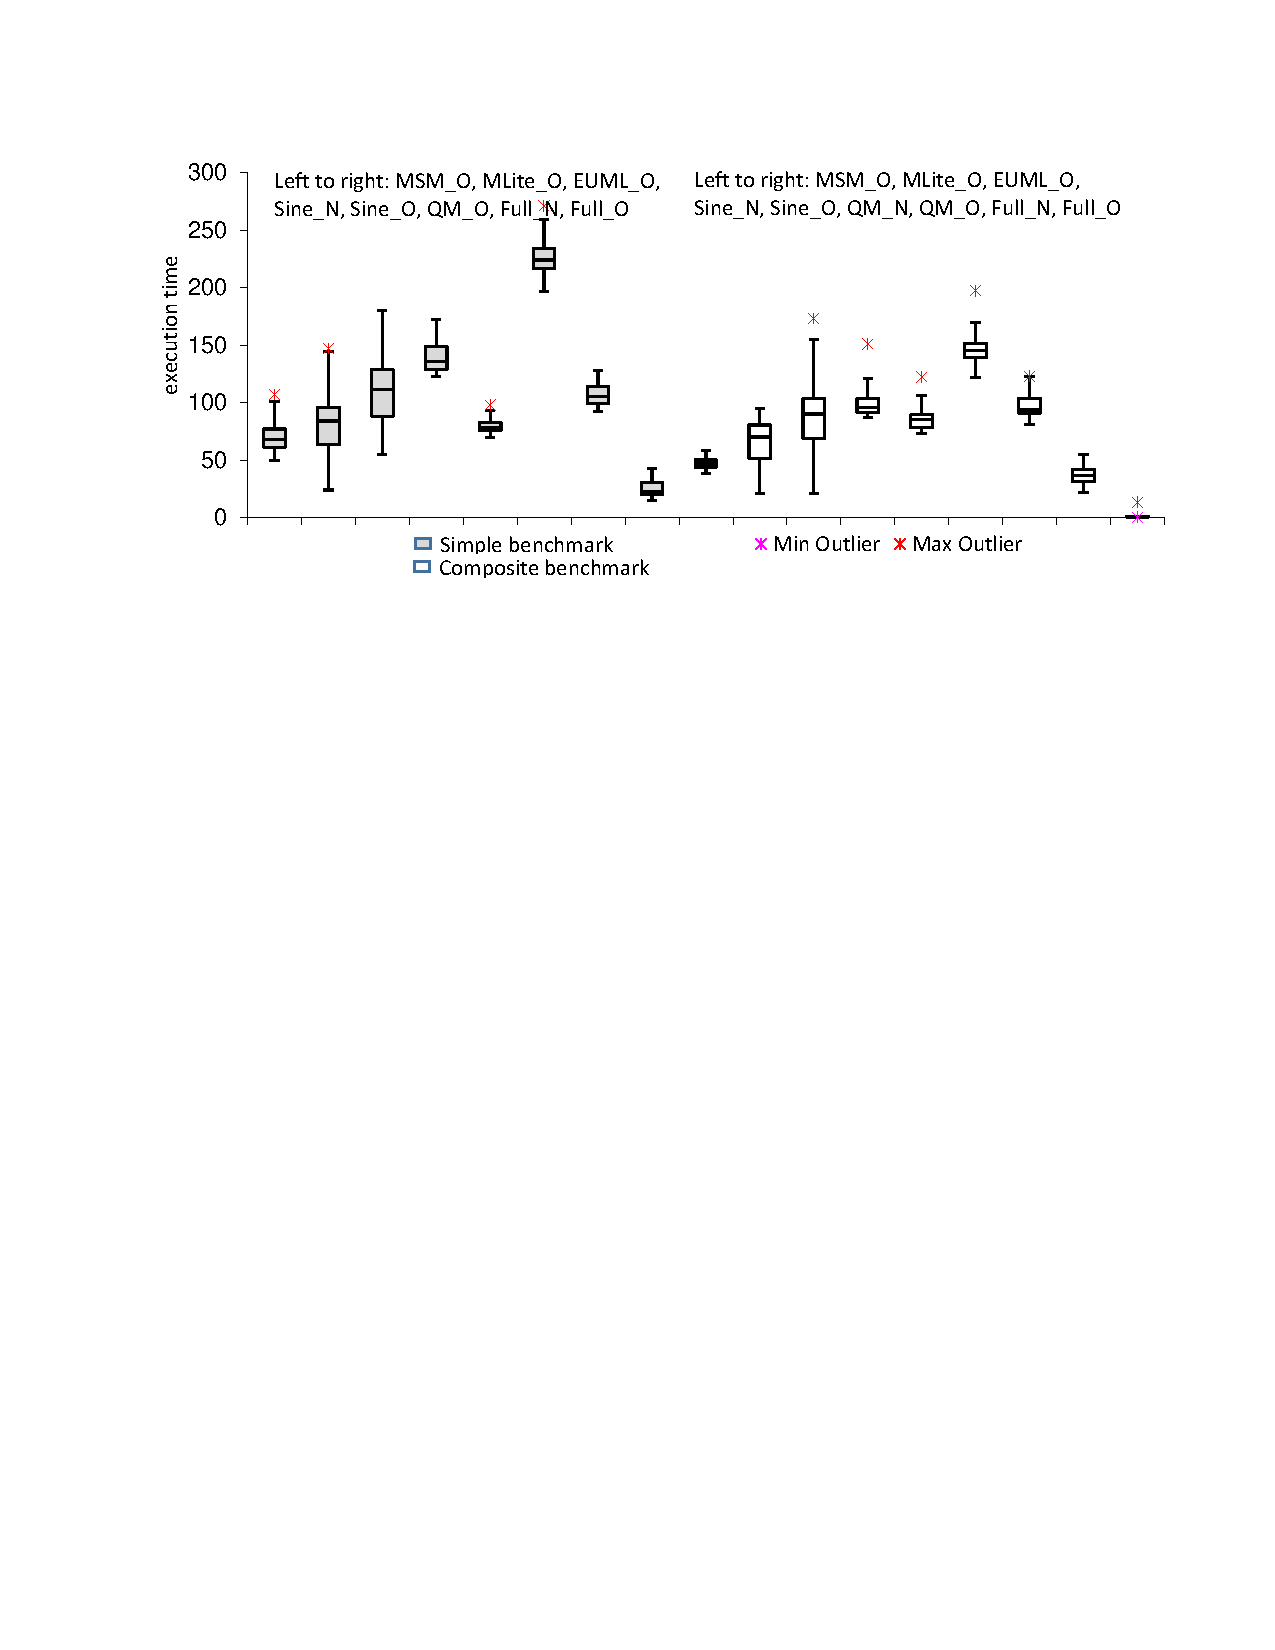
\includegraphics[clip, trim=2.8cm 18.0cm 1.7cm 2.5cm, width=\columnwidth]{experiments/box-plot-mine.pdf}
	\caption{Event processing speed for the benchmark} 
	\label{fig:boxplot}
\end{figure}

\subsubsection{Binary size and runtime memory consumption} 
Table \ref{table-size} shows the executable size for the examples compiled in two modes.
It is seen that, in GCC normal mode, Sinelabore generates the smallest executable size while our approach takes the second place.
When using the GCC optimization options, QM and our approach require less static memory than others. 

Considering runtime memory consumption, we use the Valgrind Massif profiler\cite{Massif} to measure memory usage. 
Table \ref{table:usage} shows the measurements for the composite example. 
Compared to others, code generated by our approach requires a slight overhead runtime memory usage (1KB).
This is predictable since the major part of the overhead is used for C++ multi-threading using POSIX Threads and resource control using POSIX Mutex and Condition. 
However, the overhead is small and acceptable (1KB). 


\begin{comment}
\begin{table*}[]
	\centering
	\caption{Executable size in Kb}
	\label{table-size}
	\begin{tabular}{|l|l|l|l|l|l|l|l|l|l|l|l|l|l|l|l|l|}
		\hline
		\multirow{2}{*}{Test} & \multicolumn{2}{c|}{SC} & \multicolumn{2}{c|}{MSM} & \multicolumn{2}{c|}{MSM-Lite} & \multicolumn{2}{c|}{EUML} & \multicolumn{2}{c|}{Sinelabore} & \multicolumn{2}{c|}{QM} & \multicolumn{2}{l|}{Umple} & \multicolumn{2}{c|}{Our approach} \\ \cline{2-17} 
		& N           & O         & N           & O          & N              & O            & N            & O          & N              & O              & N          & O          & N            & O           & N               & O               \\ \hline
		Simple                & 320      & 63,9     & 414,6      & 22,9      & 107,3         & 10,6        & 2339      & 67,9      & 16,5          & 10,6          & 22,6      & 10,5      &       X       &       X      & 21,5           & 10,6           \\ \hline
		Composite             & 435,8      & 84,4     & 837,4      & 31,1      & 159,2         & 10,9        & 4304,8      & 92,5      & 16,6          & 10,6          & 23,4      & 21,5      & X           & X          & 21,6           & 10,6           \\ \hline
	\end{tabular}
\end{table*}
\end{comment}

\begin{table*}[]
	\centering
	\caption{Executable size in Kb}
	\label{table-size}
	\begin{tabular}{|l|l|l|l|l|l|l|l|l|l|l|l|l|l|l|}
		\hline
		\multirow{2}{*}{Test} & \multicolumn{2}{c|}{SC} & \multicolumn{2}{c|}{MSM} & \multicolumn{2}{c|}{MSM-Lite} & \multicolumn{2}{c|}{EUML} & \multicolumn{2}{c|}{Sinelabore} & \multicolumn{2}{c|}{QM} & \multicolumn{2}{c|}{RAOES} \\ \cline{2-15} 
		& N           & O         & N           & O          & N              & O            & N            & O          & N              & O              & N          & O          & N           & O          \\ \hline
		Simple                & 320         & 63,9      & 414,6       & 22,9       & 107,3          & 10,6         & 2339         & 67,9       & 16,5           & 10,6           & 22,6       & 10,5       & 21,5        & 10,6       \\ \hline
		Composite             & 435,8       & 84,4      & 837,4       & 31,1       & 159,2          & 10,9         & 4304,8       & 92,5       & 16,6           & 10,6           & 23,4       & 21,5       & 21,6        & 10,6       \\ \hline
	\end{tabular}
\end{table*}

%\subsubsection{Runtime memory consumption}

\begin{table}[]
	\centering
	\caption{Runtime memory consumption in KB. Columns (1) to (7) are SC, MSM, MSM-Lite, EUML, Sinelabore, QM, and our approach, respectively.}
	\label{table:usage}
	\begin{tabular}{|l|l|l|l|l|l|l|l|l|}
		\hline
		Test      & (1)    & (2)  & (3) & (4) & \begin{tabular}[c]{@{}l@{}}(5)\end{tabular} & (6)    & \begin{tabular}[c]{@{}l@{}}(7)\end{tabular} \\ \hline
		Composite & 76.03 & 75.5 & 75.8  & 75.5 & 75.8                                                  & 75.7      & 76.5                                                   \\ \hline
	\end{tabular}
\end{table}


%\lipsum[1-6]

\section{Comparison and Related work}
\label{sec:relatedwork}
%\subsection{Model-code synchronization}
%Several commercial and open-source tools \cite{EA, ibm_rational_2016, Magicdraw, umlgen} support round-trip engineering between UML models and code.
%Systematic reviews of some of these tools are available in \cite{Cutting2015}.
%Support for Java round-trip is prominent in most tools.
%Other languages such as C++ are only available in a few tools \cite{ibm_rational_2016, umlgen, Magicdraw}.
%Our methodological pattern does not focus on a particular programming language
%or a particular modeling language. Furthermore, the current implementation of our approach is dedicated
%to UML and C++, which is less supported by tools than Java.
%Usually these tools only support architectural elements on the model-side.
%The model cannot be used for full implementation and
%dependencies derived from
%method bodies are not considered during the round-trip. In our work, we assume that
%the model can be used for full implementation. Furthermore, our implementation analyzes
%C++ method bodies not only to reverse them to UML, but also to derive dependencies in the UML model.
%Some tools \cite{EA} only allow
%one of the artifacts, model or code, to be edited at a certain time.
%There is then no problem of synchronizing model and code since there are no concurrent changes, which limits their applicability.
%Finally, some tools \cite{umlgen} do not support a real incremental reverse or code generation;
%instead, they treat change (e.g. renaming) as deletion followed by addition.

% RTE restriction
\subsection{Round-trip engineering and co-evolution}
Some RTE techniques restrict the development artifact to avoid
synchronization problems.
Partial RTE and protected regions are introduced in \cite{czarnecki_multi-level_2006} to preserve code editions which cannot be propagated to models.
The mechanisms as discussed in Section \ref{sec:intro} are used for the separation of generated and non-generated code. 
EMF implements these techniques to allow users to embed user-code replacing the default generated code.
Yu et al. \cite{yu2012maintaining} propose to synchronize user-code and generated code through bidirectional transformation.
This latter does not, however, allow modifications in regions beyond the marked ones and thus prohibits the programmers from changing USMs' topology.
\ttt{Deep separation} proposed in \cite{zheng2012enhancing} overcomes the limitations of the separation mechanisms.
However, %as the authors state that, 
it does not allow to modify the system architecture at the code level as previously discussed.  
%Furthermore, as discussed in Section \ref{sec:intro}, there is still a possibility for the programmers to produce accidental changes, which cannot be reflected to the model.  




In \cite{kramer2015change}, source code and component model can be derived as views from a super model for modifications in an editor for co-evolution.
However, code modifications made outside of their (limited) editor and violating their rules, e.g. only method bodies allow to be modified in code, are not updated to the super model. 
 
In \cite{Maro:2015:IGT:2814251.2814253}, the authors integrate graphical and textual editors for UML profiles to allow developers to work in both of the representations.
However, this approach is dependent and embeds all modeling concepts to textual editors while XSeparation only introduces partially to keep programmers being familiar with of their favorite programming language.

In \cite{angyal_synchronizing_2008} a three-way merging approach is proposed to synchronize code with platform specific models.
However, it only deals with syntactic synchronization while the code semantics such as state machines in source code is not taken into account.

%\paragraph{Viewpoint synchronization}
%
%% Viewpoint
%Both models and code can be considered simply as different viewpoints
%of the same system. Viewpoints enable the partitioning of the model of a system into several representations. 
%Synchronization between viewpoints is crucial to maintain their consistency.
%
%In \cite{eramo_change_2008} the authors improve the modeling of relationships and constraints between
%elements in different viewpoints in order to better guarantee the consistency of viewpoints.
%In \cite{goedicke_viewpoint-oriented_2000} the authors argue that inconsistencies will exist
%in systems developed with different actors, using different viewpoints. They suggest that tools
%must be able to tolerate inconsistencies. A distributed graph transformation is proposed to deal with the problem of formalizing the integration of multiple viewpoints in software development.
%Their work focuses on requirements engineering.
%In contrast, our approach targets specifically both model and code.
%Code is not usually considered in viewpoint synchronization because code is deemed to be too fine-grained.
%Furthermore, our approach does not require explicit modeling
%of relationships between model and code elements.

%\subsection{Model synchronization}

%Viewpoints synchronization is generalized by model synchronization for which there is
%an abundance of techniques presented in the literature. 
%Model synchronization aims
%to maintain consistency between a source model and a target model. 

\begin{comment}

Many model synchronization techniques require the explicit mapping of source model and target model.
The authors in \cite{Paesschen2005} propose an injective mapping of elements in the source model to
the target model. The mapping can be used for synchronization.
Techniques and technologies, such as Triple Graph Grammar (TGG) \cite{giese_incremental_2006},
and QVT-Relation \cite{Omg2008},
allow synchronization between source and target elements that have non-injective mappings.
The authors in \cite{Hermann2012} formalize TGG for synchronization of models that are concurrently edited.
All of these techniques require a mapping model to connect the source and target models
with typed traceability links, which need to be persisted in a model store \cite{Bergmann2011}.
This means that editing one model requires the presence of the other.
Our model-code synchronization approach does not require a mapping model and an artifact may be edited
independently of the presence of the other corresponding artifact.

Other techniques \cite{foster_combinators_2007} are based on bi-directional transformations, which comprise a forward transformation of
source to target model, and a backward transformation of target to source model.
Bi-directional transformations provides a novel mechanism for synchronization.
Indeed, some works \cite{Matsuda2015} derive a backward transformation based on forward
transformation.
However, such works do not offer any means to synchronize models that are concurrently edited.

A few approaches derive model synchronization from model transformation while allowing concurrent editions
of both source and target models.
In \cite{xiong_towards_2007} the authors propose to automatically derive
model synchronization of a source and a target model related by
%an ATL \cite{eclipse_foundation_eclipse_2016}
model transformation.
The synchronization is based on differentiating source and target model states
but reflectable addition of an element in the target model is not well handled according to \cite{xiong_towards_2007}.
Our approach is generic and does not depend on a specific technology. Furthermore, in our implementation
we propose to use modification events rather than state differences for incremental
transformations, necessary for synchronization.

\end{comment}

%\subsection{State machine code generation}

%\label{sec:relatedwork}
%Code generation from state machines has been received huge attention in automated software development and many approaches are proposed. 
%This section mentions some usual patterns and how our approach differs. 
%A systematic review of proposals is presented in \cite{Domnguez2012}. 
%Main approaches including switch/if, state table and state pattern are investigated.

%Switch/if is the most intuitive technique implementing a "flat" state machine. Two types of switch/if are supported. The first one uses a scalar variable representing the current active state \cite{Booch1998}. A method for each event processes the variable as a discriminator in switch/if statement. The second one uses a double nested switch/if and has two variables to represent the current active state and the event to be processed \cite{Douglass1999}. The latter are used as the discriminators of an outer switch statement to select between states and an inner one/if statement to decide how the event should be processed. The behavior code of the two types is put in one file or class. This practice makes code cumbersome, complex, difficult to read and less explicit when the number of states grows or the state machine is hierarchical. Furthermore, the first approach lets the code scatter in different places. Therefore, maintaining or modifying such code of complex systems is very difficult.

%Many techniques for code generation from USM are proposed.
%Switch/if %is the most intuitive technique implementing a "flat" state machine \cite{Booch1998}.
%and double dimensional state table approach \cite{Douglass1999} are intuitive and efficient techniques. 
%one dimension represents states and the other one all possible events. 
%These usually require a transformation from hierarchical to flatten ones and support only a small subset of USM concepts such as state and transition.
%However, the semantics of USMs containing pseudo states such as histories or join/fork are hardly preserved during the transformation. 
%The latter can be implemented by either
%using a scalar variable \cite{Booch1998} and a method for each event or using two variables as the current active state and the incoming event used as the discriminators of an outer switch statement to select between states and an inner one/if statement, respectively. 
  
%Each cell of the table is associated with a function pointer meaning that the state associated with a dimension index of the cell is triggered by the event associated with the other dimension. 
%The behavior code of these techniques is put in one file or class. This practice makes code cumbersome, complex, difficult to read and less explicit when the number of states grows or the state machine is hierarchical. 
%Therefore, maintaining or modifying such code of complex systems is very difficult. 
%Furthermore, these approaches requires every transition must be triggered by at least an event. This is obviously only applied to a small sub-set of USMs.  

%Some approaches such as state pattern \cite{Shalyto2006,Douglass1999} and its extension \cite{niaz_mapping_2004} produce object-oriented code by representing states as classes.
% to implement flat state machines. Each state is represented as a class and each event as a method. %The event is processed by a delegation from the context class to sub-states. 
%Separation of states in classes makes the code more readable and maintainable. %Unfortunately, this technique only supports flat state machines. 
%This pattern is extended in \cite{niaz_mapping_2004} to support hierarchical-concurrent USMs. 
%Recently, a double-dispatch (DD) pattern presented in \cite{spinke_object-oriented_2013} extends \cite{niaz_mapping_2004} to support maintainability. %by as a new technique to implement state machines. 
%representing states and events as classes, and transitions as methods. 
%However, these approaches do not generate code for full USM features and require much memory because of class explosion and uses dynamic memory allocation, which is not preferred in embedded systems \cite{spinke_object-oriented_2013}.
%However, the maintenance of the code generated by this approach is not trivial since it requires many small changes in different places. %This is impractical when dealing with large state machines. %Furthermore, similar to the state table, this approach also poses the requirement of having at least one event for transition.

%Tools, such as \cite{ibm_rhapsody, sparxsystems_enterprise_2014}, apply different patterns to generate code. 
%However, as mentioned in Section \ref{sec:intro}, true concurrency and some pseudo-states are not supported. 




%Our generation approach relies on and extends this approach. The latter profits the polymorphism of object-oriented languages. %provides some 1-1 mappings from state machines to object-oriented code and the implementation technique 
%is not dependent on a specific programming language. 
%However, DD does not deal with triggerless transitions and different event types supported by UML such as \ti{CallEvent}, \ti{TimeEvent} and \ti{SignalEvent}. Furthermore, DD is not a code generation approach but an approach to manually implementing state machines.




\subsection{Language engineering}
Text-based modeling languages (Textual ML) of UML such as PlantUML \cite{plantuml}, Umple \cite{lethbridge2010umplification}, and Earl Grey (EG) \cite{mazanec2012general} support UML class and State Machine elements.
However, these languages lack the explicit support for event types definitions used in UML.
Furthermore, they 
do not allow the programmers to reuse the existing syntax of object-oriented languages but redefine it in their own language and IDE, which is different with the idea of considering OOL as a hosting language and additional constructs as an internal language. 
By this way, Textual MLs need a tooling support such as compiler and editor, which require a lot of engineering tasks to develop. 
Contrarily, XSeparation only requires a light-weight compiler and enables using favorite IDEs. %while familiarity of these Textual MLs are questionable in \cite{mazanec2012general}. 
%XSeparation automatically synchronizes the code with the system model specified by UML.
%Hence, XSeparation profits all benefices of IDEs such as intelligent completion and easy to implement. 
Furthermore, XSeparation allows to use all specific OOL features such as pointers and references in C++ for program performance.%, which are not available in the Textual MLs.
%Followings list differences in comparison between RAOES and the TMLs.

\begin{comment}
\begin{itemize}[\footnotesize]
	\item RAOES adapts USM features to existing programming languages while Umple or TextUML does inversely, hence RAOES profits all benefices of IDEs such as intelligent completion and easy to implement. Furthermore, RAOES allows to use all specific C++ features such as function pointers for program efficiency, which are not available in the the TMLs.
	
	\item In RAOES, the programmers write and maintain the USM-based behavior part in the same class/file containing the active class.
	
	\item RAOES support full USM features.
	
	\item RAOES automatically synchronizes the code with the system model specified by UML.
	
	\item RAOES defines the state machine topology separately from the transition table and event definition.
\end{itemize}
\end{comment}


In \cite{Luo:2016:BIS:2997364.2997372} BSML-mbeddr is proposed as an state machine-based programming language integrated into the C language.
Big and small steps are defined in the language semantics.
However, the latter is not UML-compliant. 
BSML-mbeddr only it specifies only state and region concepts and does not allow different event types as XSeparation does. 
Furthermore, BSML-mbeddr is a code-centric approach whereas XSeparation enables a model-code concurrent development, maintenance, and co-evolution of the artifacts.  

%The idea of adding more constructs for object-oriented languages to contain architecture information in XSeparation is similar to ArchJava \cite{aldrich2002archjava} and Archface \cite{ubayashi2010archface}.
%This latter utilizes Java annotations to preserve architecture intention in the source code.
%These approaches try to embed architectural information into the code, specifically Java while RAOES integrates the behavior represented by USMs into C++ to ease the RTE problem. 
ArchJava \cite{aldrich2002archjava} adds structural component concepts such as part and port to Java. %to support the co-evolution of architecture structure and Java implementation. 
The Archface \cite{ubayashi2010archface} contract description language supports components and connectors, between design and implementation using concepts such as \ttt{pointcut} in Aspect programming to reason about the design and code correctness.
%The latter can also be realized with XSeparation because we generated code can be used to reconstruct component models.
These approaches, however, do not provide the traceability between of the architecture behavior and code.
%The user-code and generated code are not separated as in XSeparation and \ttt{1.x-way mapping} to allow modifications made in both architecture and code.
They also do not have a synchronization mechanism in case of concurrent development.
Furthermore, the communication between two ports uses method calls of object-oriented languages instead of interfaces as in UML.
In addition, while ArchJava makes it not Java anymore and facilities of Java's IDEs such as auto-completion are not aware, XSeparation-generated code can use these facilities as discussed in \ref{sec:xseparationarchitecture}.

%FXU \cite{Pilitowski2007} is the most complete tool but generated code is heavily dependent on their own library and C\# is generated.



%In \cite{balz2009embedding}, the authors embeds behavior models into Java by representing, for example, states as classes, transitions as annotations, guards as methods.
%Although the programmers can modify the code following these patterns, the code size is large because of class explosion.

%\subsection{Code generation patterns and tools}
Tools such as IBM Rhapsody \cite{ibm_rhapsody}, Enterprise Architect \cite{EA}, Papyrus-RT \cite{possepapyrusrt}, and Sinelabore \cite{sinelabore} support only the structure RTE for UML class diagram concepts and code generation from UML State Machines.
Techniques for generating code from USM such as SWITCH/IF, state table \cite{Douglass1999} and state pattern \cite{Shalyto2006,niaz_mapping_2004} are proposed. 
A systematic review of code generation approaches is presented in \cite{Domnguez2012}.
%Switch/if %is the most intuitive technique implementing a "flat" state machine \cite{Booch1998}.
%and state table approach \cite{Douglass1999} are intuitive techniques. 
%Some approaches such as state pattern \cite{Shalyto2006,niaz_mapping_2004} produce object-oriented code.
% to implement flat state machines. Each state is represented as a class and each event as a method. %The event is processed by a delegation from the context class to sub-states. 
%Separation of states in classes makes the code more readable and maintainable. %Unfortunately, this technique only supports flat state machines. 
%This pattern is extended in \cite{niaz_mapping_2004} to support hierarchical-concurrent USMs. 
%Recently, a double-dispatch (DD) pattern presented in \cite{spinke_object-oriented_2013} extends \cite{niaz_mapping_2004} to support maintainability. %by as a new technique to implement state machines. 
%representing states and events as classes, and transitions as methods. 
However, only a subset of USM features is supported and generated code is not efficient, %of class explosion and uses dynamic memory allocation, 
which cannot be used for embedded systems \cite{spinke_object-oriented_2013}.
%Our source-to-source transformation combines SWITCH/IF the pattern in \cite{niaz_mapping_2004} to produce small footprint and preserve state hierarchy.
%Furthermore, 
RAOES offers code generation for all USM concepts. %including states, pseudo states, transitions, and events.
Therefore, users are free and flexible to create there USM conforming to UML without restrictions.

\section{Conclusion}
\label{sec:conclusion}
We have presented a bidirectional mapping between code and architecture model specified by UML class, composite structure, and state machine diagrams.
%a round-trip engineering approach for effective collaboration between software architects and programmers in developing and maintaining reactive embedded systems using UML State Machines for describing behaviors. 
%The design for concurrency of generated code is based on multi-thread.
%The code generation pattern set extends the IF-ELSE/SWITCH patterns and the state pattern extension. 
%The hierarchy of USM is kept by our simple state structure.
%XSeparation code generation improves the bidirectional traceability between architecture model and code by proposing to generate code at an appropriate level of abstraction. 
The idea is to raise the abstraction level of an existing programming language in order to reduce the abstraction gap between modeling and coding.
The mapping is used as input in our model-code synchronization mechanism presented in \cite{foster2016}.
%An XSeparation compiler was developed to compile the XSeparation-generated code.
%XSeparation is implemented as an extension of the Papyrus modeling tool for the case of UML and C++. 

%We successfully applied XSeparation to the development of a case study.
%The latter is an software application for LEGO.
  

For the moment, the approach is implemented for UML and C++.
In the future, we will extensively evaluate the approach for different aspects: synchronization correctness, feasibility, and scalability. 
Furthermore, we will apply our approach to other programming languages such as Java and C\# and investigate how this work may scale on modern architectures. 
%\lipsum[1-2] 
%RAOES introduces a C++ front-end code lying between models and actual executable code.
%RAOES proposes a framework for synchronizing the models and the front-end code, and generating executable code from the front-end.
%RAOES is implemented as an extension of the Papyrus modeling tool.

%We evaluated RAOES by conducting experiments on the round-trip engineering correctness, the semantic-conformance and efficiency of generated code, and by implementing a case study simulation of a Traffic Light Controller.
%300 random models are tested for the RTE correctness.
%The conformance is tested under PSSM: 62/66 tests pass.
%The efficiency of back-end code has been evaluated, RAOES produces code that runs faster in event processing time and is smaller in executable size than those of other approaches (in the paper's scope).

%Although RAOES does not deal with extraction of information from existing/legacy code, the latter can still be reused by RAOES in two ways: (1) reverse engineering from the legacy code to a model, which can be manipulated further by architects, or (2) directly integrating the legacy code by programmers into front-end code. 
%Furthermore, RAOES allows to work abstractly by using models and in a low-level way by using front-end code concurrently and simultaneously. Hence, RAOES is effective in software development, evolution, collaboration, and maintenance by using our synchronization process.


%For the moment, RAOES supports the co-evolution of UML class and state machine diagrams and code.
%In the future, we will integrate component-based concepts into C++ to make the front-end more powerful and effective.
%Our wish is to embed component-connector and interaction component information represented in UML composite structure diagrams into C++ to elaborate the application range such as distributed embedded systems.
%A possible direction to this integration is to extend \ttt{nesc} \cite{gay2003nesc} - an extension of the C language dedicated component-based development of networked applications.
%However, code produced by PSM consumes slightly more memory than the others.
%Furthermore, some PSSM tests are failed.
%Therefore, as a future work, we will fix these issues by making multi-thread part of generated code more concise.  
 

%\section*{Appendix}
%Appendixes, if needed, appear before the acknowledgment.

%\section*{Acknowledgment}
%This work is motivated by....


\balance
\bibliographystyle{IEEEtran}
\bibliography{refs}



\end{document}
